\documentclass[compress, ucs, xelatex, 11pt, xcolor=svgnames,
  hyperref={
    bookmarks=true,
    unicode=true,
    colorlinks=true,
    pdftitle={Linux, command line and MetaCentrum},
    plainpages=false,
    pdfauthor={Vojtech Zeisek},
    pdfsubject={Course about use of Linux command line, writing shell scripts and using MetaCentrum of CESNET},
    pdfcreator={XeLaTeX},
    pdfkeywords={Linux, GNU, BASH, shell, command line, MetaCentrum},
    linkcolor=DarkRed,
    anchorcolor=DarkBlue,
    citecolor=Indigo,
    filecolor=NavyBlue,
    menucolor=DarkMagenta,
    urlcolor=DarkBlue,
    pdftex},
  url={hyphens, lowtilde} % Allow line breaks within URLs
  ]{beamer}

% Theme settings
\usetheme[secheader]{Boadilla}
\usecolortheme{spruce}
\setbeamertemplate{headline} {
  \begin{beamercolorbox}{section in head/foot}
    \insertsectionnavigationhorizontal{\paperwidth}{\hskip0pt plus1fill}{\hskip0pt plus1fill}
  \end{beamercolorbox}
  \begin{beamercolorbox}[ht=2ex, dp=1.125ex]{subsection in head/foot}
    \insertsubsectionnavigationhorizontal{\paperwidth}{}{\hfill\hfill}
  \end{beamercolorbox}
  }
\useinnertheme{circles}

% Basic packages
\usepackage{xltxtra} % Loads following 3 packages for processing with XeLaTeX
\usepackage{metalogo}
\usepackage{xunicode}
\usepackage{fontspec}

% Other packages
\usepackage{multicol}
\usepackage{tabularx}

% In-line higlighting
\usepackage{soul}

% Add background for \texttt{} (using pacakge soul)
\sethlcolor{Beige}
\renewcommand{\texttt}[1]{\hl{\ttfamily #1}}

% Change text color of highlighted text back to red
\renewcommand{\alert}[1]{\textcolor{red}{#1}}

% Syntax higlight
\usepackage{minted}
\usemintedstyle{vim} % Styles are listed by pygmentize -L styles; languages are listed by pygmentize -L lexers
\newminted{bash}{linenos, fontsize=\footnotesize, bgcolor=Beige, fontfamily=tt, gobble=4, numbersep=-6pt}
% Change line number style
\renewcommand{\theFancyVerbLine}{
  \sffamily
  \textcolor{BlueViolet}{
    \tiny
    \oldstylenums{
      \arabic{FancyVerbLine}
      }
    }
  }

% Fixing space before and after block of code higlight
\BeforeBeginEnvironment{bashcode}{\vspace{-1em}}
\AfterEndEnvironment{bashcode}{\par\vspace{-1em}}

% Fixing space before and after multicols region
\BeforeBeginEnvironment{multicols}{\vspace{-0.5em}}
\AfterEndEnvironment{multicols}{\par\vspace{-0.5em}}

% Fixing space before and after itemize region
\BeforeBeginEnvironment{itemize}{\vspace{-0.25em}}
\AfterEndEnvironment{itemize}{\vspace{-0.25em}}

% Default language
\usepackage{polyglossia}
\setdefaultlanguage{english}

% Title page
\author{Vojtěch Zeisek}
\institute[\url{https://trapa.cz/}]{Department of Botany, Faculty of Science, Charles University, Prague\\Institute of Botany, Czech Academy of Sciences, Průhonice\\\url{https://trapa.cz/}, \href{mailto:zeisek@natur.cuni.cz}{zeisek@natur.cuni.cz}}
\title{Linux, command line \& MetaCentrum}
\subtitle{Use of Linux command line not only for CESNET's MetaCentrum}
\titlegraphic{
\includegraphics[width=2cm]{tux.png}}
\date{February 6 to 8, 2018}

\begin{document}

\begin{frame}
  \titlepage
\end{frame}

\begin{frame}[allowframebreaks]{Outline}
  \tableofcontents
\end{frame}

\section{Introduction}

\begin{frame}{The course information}
  \begin{itemize}
    \item The course page: \url{https://trapa.cz/en/course-linux-command-line-2018}
    \begin{itemize}
      \item Česky: \url{https://trapa.cz/cs/kurz-prikazove-radky-linuxu-2018}
    \end{itemize}
    \item Subject in SIS: \url{https://is.cuni.cz/studium/eng/predmety/index.php?do=predmet&kod=MB120C17}
    \begin{itemize}
      \item Česky: \url{https://is.cuni.cz/studium/predmety/index.php?do=predmet&kod=MB120C17}
      \item For students having subscribed the subject, active participation and presence whole course is required
    \end{itemize}
    \item Working version is available at \url{https://github.com/V-Z/course-linux-command-line-bash-scripting-metacentrum} -- feel free to contribute, request new parts or report bugs
  \end{itemize}
\end{frame}

\begin{frame}{Materials to help you\ldots}
  \begin{itemize}
    \item Download the presentation from \url{https://soubory.trapa.cz//linuxcourse/linux_bash_metacentrum_course.pdf}
    \item Download the scripts and toy data from \url{https://soubory.trapa.cz/linuxcourse/scripts_data.zip}
    \begin{itemize}
      \item \alert{Note:} Open the scripts in some \alert{good} text editor (slide~\ref{editors}) -- showing syntax highlight, line numbers, etc. (\alert{NO} Windows notepad); the files are in UTF-8 encoding and with UNIX end of lines (so that too silly programs like Windows notepad won't be able to open them correctly)
      \item \alert{Never ever} open any script file in software like MS~Word -- they destroy quotation marks and other things by ``typographical enhancements'' making the script unusable
    \end{itemize}
  \end{itemize}
\end{frame}

\begin{frame}{Virtual machine for learning}
  \label{VBox}
  \begin{multicols}{2}
    \begin{itemize}
      \item If you do not have Linux installed, download and install VirtualBox from \url{https://www.virtualbox.org/}
      \item Download openSUSE Leap 42.2 Linux distribution for this course from \url{ftp://botany.natur.cuni.cz/openSUSE_Leap_Linux_course.ova} (3.7~GB)
      \item Launch VirtualBox and go to menu \textbf{File | Import appliance\ldots} to import it. When do, launch it (\textbf{Start})
    \end{itemize}
    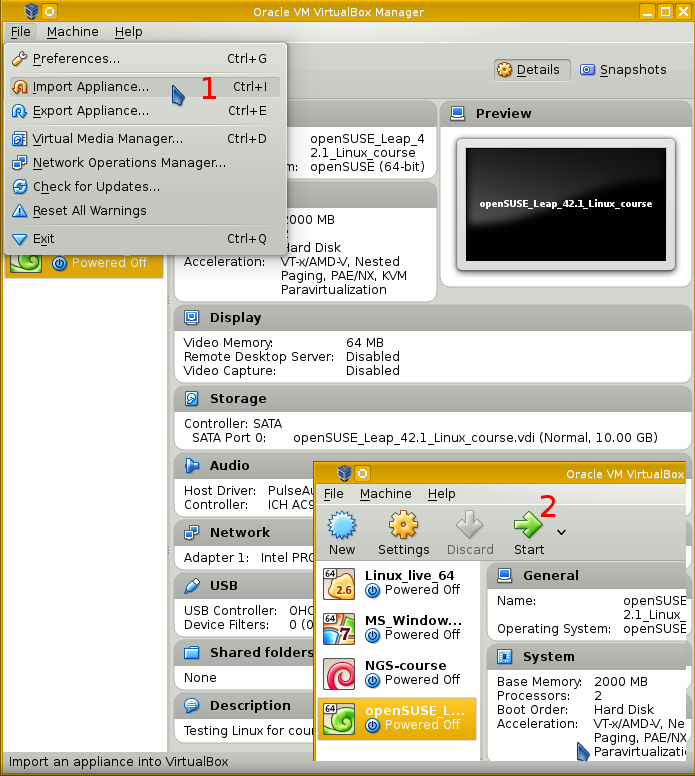
\includegraphics[height=6cm]{virtualbox.png}
  \end{multicols}
\end{frame}

\begin{frame}{VirtualBox shared folder I}{VirtualBox can be configured to share folder with host operating system}
  \begin{center}
    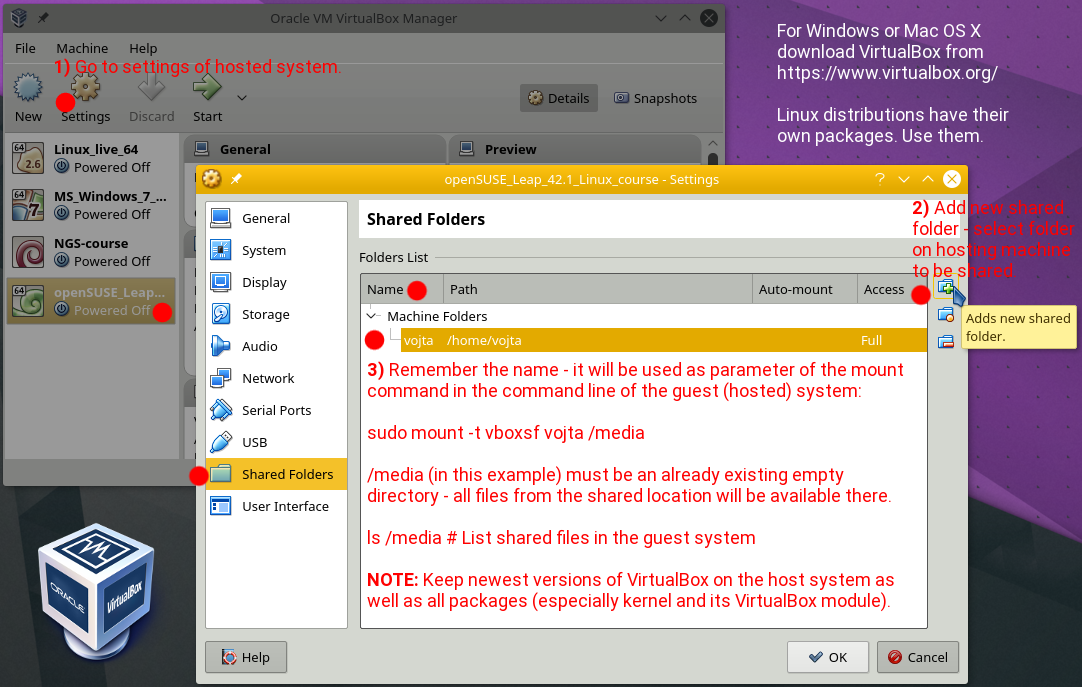
\includegraphics[width=\textwidth-2cm]{virtualbox_shared_folder_1.png}
  \end{center}
\end{frame}

\begin{frame}[fragile]{VirtualBox shared folder II}{Go to menu ``Devices | Shared Folders'' and set pair of folders}
  \begin{bashcode}
    sudo mount -t vboxsf -o uid=$UID,gid=$(id -g) shared /mnt
  \end{bashcode}
  \vfil
  \begin{center}
    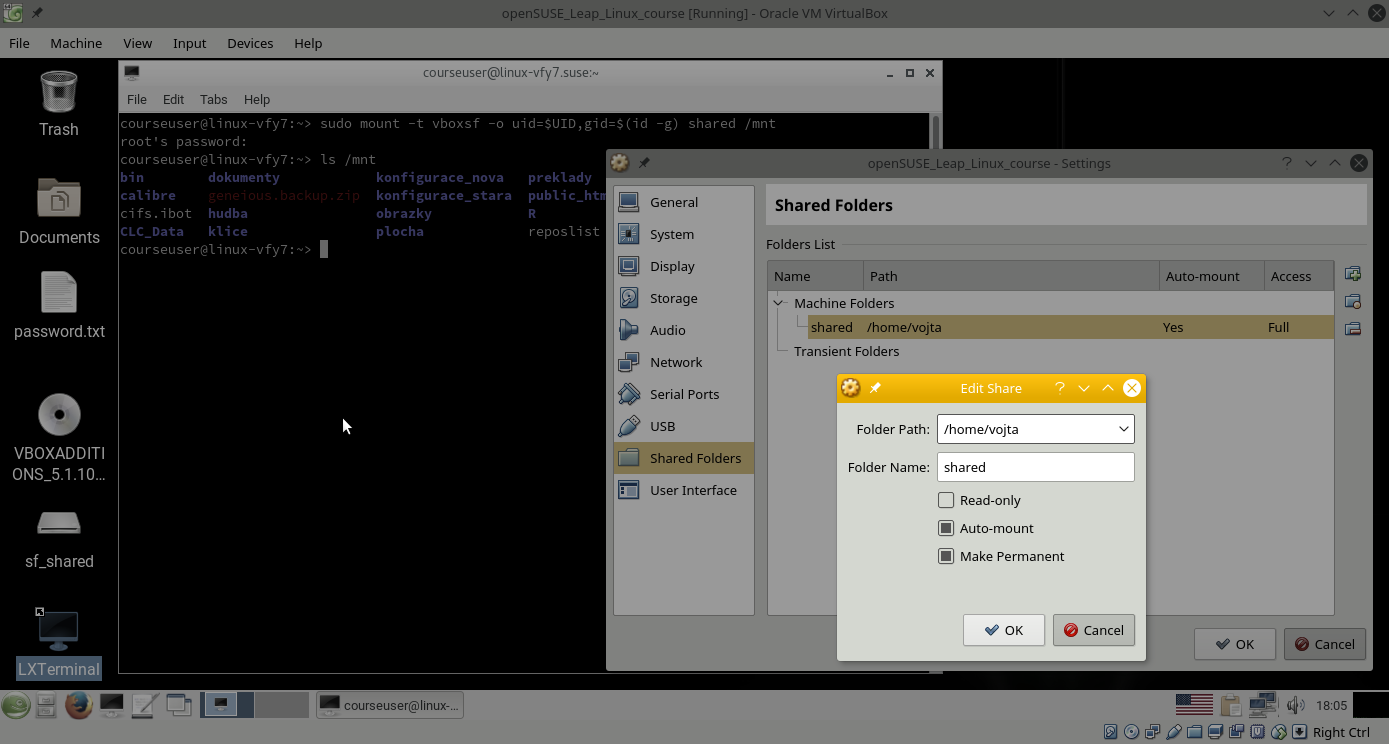
\includegraphics[width=\textwidth-1cm]{virtualbox_shared_folder_2.png}
  \end{center}
  \vfill
\end{frame}

\begin{frame}[allowframebreaks]{What it is UNIX, Linux and GNU}
  \begin{itemize}
    \item \href{https://en.wikipedia.org/wiki/Unix}{UNIX}
    \begin{itemize}
      \item Originally developed in Bell labs of AT\&T in 1696, written in C, since then  huge radiation, hybridization, HGT,~\ldots
      \item Trademark -- only systems passing certain conditions (paid certification) can be called ``UNIX'' -- Solaris, HP-UX, AIX, etc. (commercial systems for big servers)
      \item Main principles: simple, multitasking, hierarchical, network, for more users (takes cares about permissions etc.), configuration written in plain text files, important relationships among applications (generally one application = one task -- they are chained), work primarily with text, has kernel and API (interface to communicate with the rest of the system)
      \item \href{https://en.wikipedia.org/wiki/Unix-like}{UNIX-like} (UN*X, *nix)
      \begin{itemize}
	\item Systems compatible with UNIX (Linux, BSD and its variants, Mac OS~X,~\ldots)
	\item Mainly open-source (UNIX is commonly commercial -- source code is not available for public, but its specification is)
	\item Nowadays prevailing over ``old'' UNIX systems, used in many devices from tiny embedded toys to huge data centers
	\item Try to provide same quality as paid systems, but (mostly) for free
      \end{itemize}
      \item Many courts about copyrights, parts of code, patents -- USA allow software patents, EU not -- GNU, Linux, BSD, etc. try to ensure to have only code not covered by any patents to avoid possible courts
    \end{itemize}
    \item \href{https://www.gnu.org/}{GNU}
    \begin{itemize}
      \item ``GNU's Not Unix!'' -- but it is compatible, respects its principles
      \item Since 1984 Richard Stallman (founder of \href{https://www.fsf.org/}{Free Software Foundation}) tried to make new kernel (Hurd -- not finished yet\ldots)
      \item Generally set of basic system tools -- working with many kernels (Linux BSD*, Mac's Darwin,~\ldots), also present in many commercial paid UNIX systems
      \item Source code is free -- anyone can study it (Security!), report bugs, contribute, modify, share it,~\ldots
      \item GNU General Public License (GPL) -- free spirit of open-source -- license, idea, how to share software
    \end{itemize}
    \item \href{https://en.wikipedia.org/wiki/Linux}{Linux}
    \begin{itemize}
      \item First version of kernel written by Linus Torvalds in Helsinki in 1991
      \item Kernel was in principle inspired by various UNIX systems and using GNU tools for work
      \item Quickly became popular -- anyone can take it and use for any needs
      \item Used in small embedded (commonly network) devices, mobile devices (book readers, Android,~\ldots), personal computers, servers (from home level to biggest data centers),~\ldots
      \item Nowadays powering most of the Internet
      \item Anyone can contribute -- not only code, also documentation, design, translations,~\ldots
    \end{itemize}
  \end{itemize}
\end{frame}

\begin{frame}{Extremely simplified UNIX phylogeny}
  \begin{center}
    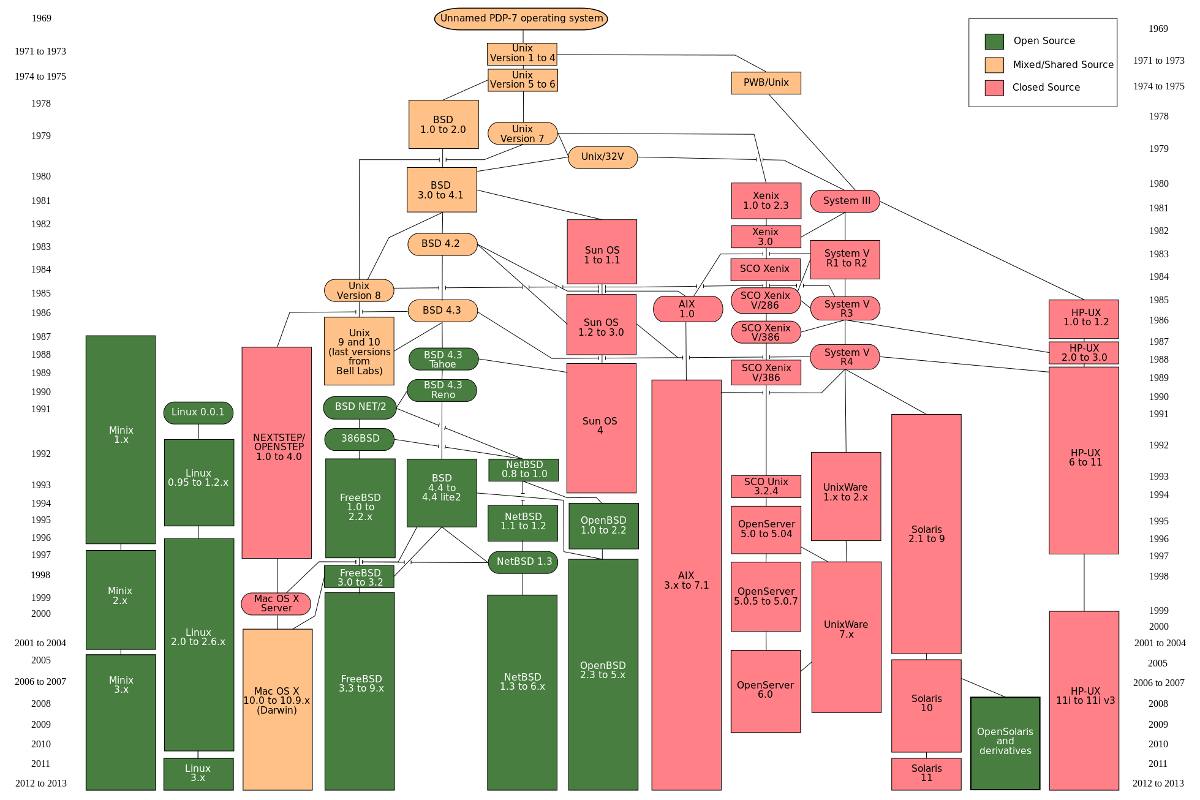
\includegraphics[height=7cm]{unix_history-simple.png}
  \end{center}
\end{frame}

\subsection{Licenses and money}

\begin{frame}{Cathedral vs. market place}{What is principal difference between free open-source and commercial software}
  \begin{itemize}
    \item Commercial software is like a cathedral
    \begin{itemize}
      \item Pay big money and get it in the state which the architect like
      \item User can not modify it (or it is terribly expensive)
      \item Might be you don't need everything -- but still paying whole set
    \end{itemize}
    \item Free open-source software (FOSS) is like a market place
    \begin{itemize}
      \item Find there many producers of same tools -- pick up those you like -- freedom of choice
      \item Take exactly the tools you need -- any combination is possible
      \item Much cheaper to shop there
    \end{itemize}
    \item Both have pros and cons -- depends what you wish\ldots
  \end{itemize}
\end{frame}

\begin{frame}[allowframebreaks]{Free and open-source software -- (F)OSS}
  \begin{itemize}
    \item \textbf{Free like freedom of speech, \alert{not} like free beer!}
    \item Not every OSS (generally less strict conditions) has to be \textbf{F}OSS (you can do with it (almost) whatever you like) -- source code might be available under some circumstance (only to look), but modification and/or reuse of the code prohibited (and then it is not \textbf{free})
    \item Open-source -- source code can be seen by the holder of the license -- many variants of exact conditions
    \item GNU GPL (``\href{https://www.gnu.org/copyleft/}{copyleft}'') -- probably most common OSS license, strict, viral -- derived code has to keep the license -- surprisingly not fully ``free'' as it doesn't allow changes of license
    \item LGPL -- Lesser GPL -- more permissive
    \item BSD license -- permissive -- allow derived code to became closed-source (commonly used by Apple Mac OS~X, Safari browser,~\ldots)
    \item Apache license, Mozilla license, etc. -- many variants for specific use in particular software
    \item Creative Commons (CC) -- software licenses above not suitable for multimedia, text, etc. -- CC has many options (including denial of reuse of the product), see \url{https://creativecommons.org/}
    \item And many more\ldots
    \item Orientation might be tricky, but practical output for users is more or less same -- the software can be independently checked for bugs, backdoors, malware, can be improved and under some circumstances, new software can be derived, and usually, it is available for free
    \item Aim is to ``liberate'' software to keep open sharing of ideas, mutual improve and security control -- although the point is clear, there are debates how to reach it\ldots
  \end{itemize}
\end{frame}

\begin{frame}{How to make money with free open-source software?}
  \begin{itemize}
    \item Traditional model -- user rents right (``buys a license'') to use the software (and sometimes for support -- usually for extra money)
    \item Common mistake -- software is not ``bought'' -- only license is rented (``permission to use it'')
    \item Software as service
    \begin{itemize}
      \item (F)OSS is available for free -- user can use it as it is or buy a support -- help of any type
      \item No vendor lock-in -- user has the code, so he can modify the software himself, change provider of the services,~\ldots
      \item Cheap for user as well as company -- company specialized for one task, let's say server database, doesn't have to take care about the rest of the system -- someone else does; user pays only what he needs
      \item Our faculty is using \href{https://plone.org/}{Plone} system for web pages -- anyone can use it for free, someone (like we) asked a company to help, and if we'd decided, we  could keep Plone and maintain it ourselves or find another company to help us with it
    \end{itemize}
  \end{itemize}
\end{frame}

\section{Linux}

\begin{frame}{What it is a ``Linux''}
  \begin{itemize}
    \item Operating system respecting principles of UNIX
    \item Components
    \begin{itemize}
      \item Linux kernel -- basic part of the system responsible for hardware and very basic low-level running of the system (``Linux \textit{sensu stricto}'')
      \item GNU core utilities -- basic applications
      \item Graphical user environment (GUI) -- many choices
      \item Many other applications -- according to use -- whatever imaginable
    \end{itemize}
    \item Linux distribution (``Linux \textit{senso lato}'')
    \begin{itemize}
      \item Somehow assemble Linux kernel, basic tools and some applications
      \item Optionally add some patches and extra tools and gadgets
      \item Make your own design! (very important)
      \item If lazy, remake existing distribution (using e.g. \href{https://susestudio.com/}{web service})
      \item Still surprised there are hundreds of them?
      \item It is like Lego -- pieces are more or less same across distributions, but result is very variable
      \item From ``general'' for daily use (pick up whatever you like) to very specialized -- special hardware devices, network services, rescue,~\ldots
    \end{itemize}
  \end{itemize}
\end{frame}

\begin{frame}{Linux kernel and other part around it}
  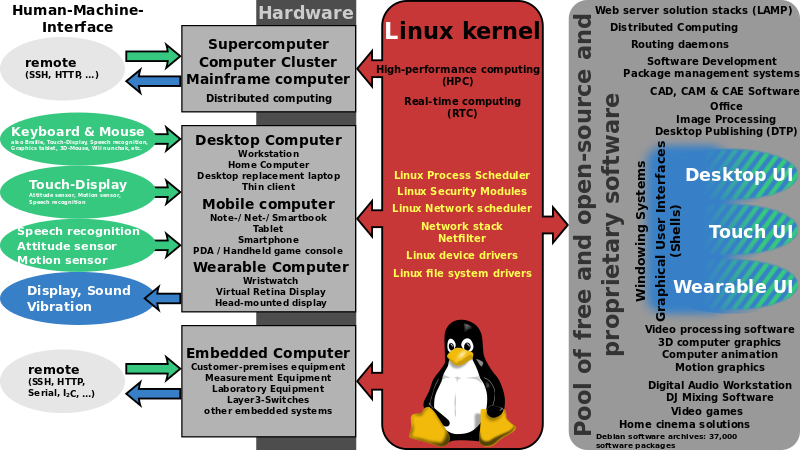
\includegraphics[width=\textwidth]{linux_kernel_ubiquity.png}
  \vfil
  \url{https://en.wikipedia.org/wiki/Linux_distribution}
  \vfill
\end{frame}

\begin{frame}{Extremely simplified adaptive radiation of Linux distributions}
  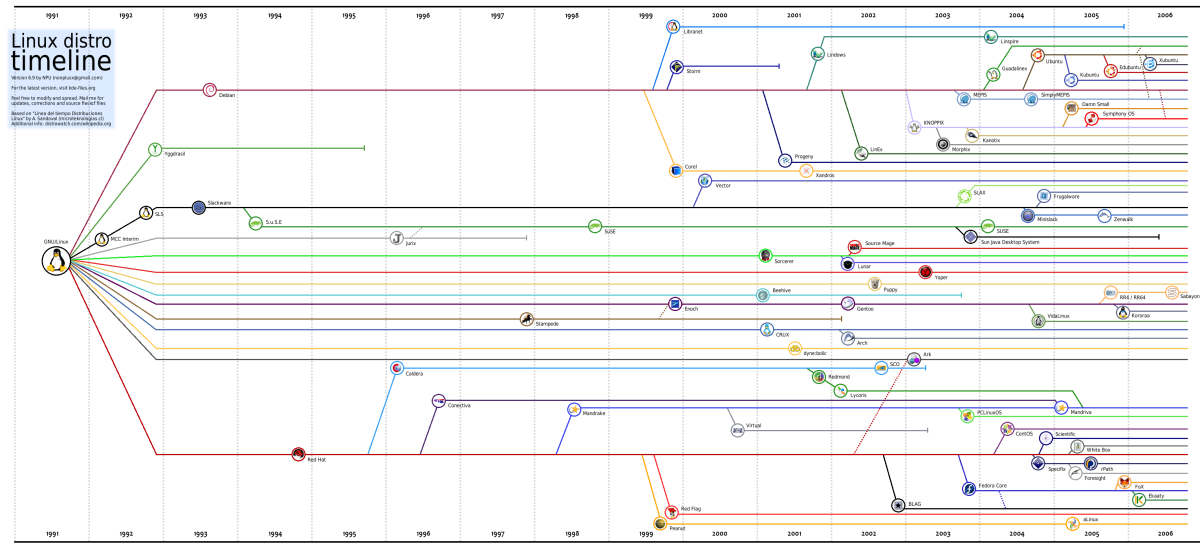
\includegraphics[width=\textwidth]{linux_fylogen_2.png}
  \vfil
  \url{https://en.wikipedia.org/wiki/List_of_Linux_distributions} and \url{https://distrowatch.com/} ($\sim$800 distributions, $\sim$260 active)
  \vfill
\end{frame}

\subsection{Choose one}

\begin{frame}{Most common Linux distributions}
  \begin{itemize}
    \item \href{http://distrowatch.com/search.php?package=DEB}{Debian (DEB) based}
    \begin{itemize}
      \item \href{https://www.debian.org/}{Debian} -- one of oldest and most common, especially on servers
      \item \href{http://www.ubuntu.com/}{Ubuntu} (nowadays probably the most popular on PCs and notebooks) and derivatives -- \href{https://www.kubuntu.org/}{Kubuntu}, \href{https://xubuntu.org/}{Xubuntu}, \href{http://lubuntu.net/}{Lubuntu},~\ldots~(according to GUI used -- most of the system is same)
      \item \href{http://linuxmint.com/}{Mint} -- Based on Ubuntu as well as Debian, very user-friendly
      \item \href{https://www.kali.org/}{Kali}, \href{http://knopper.net/knoppix/index-en.html}{KNOPPIX}, \href{https://elementary.io/}{elementaryOS},~\ldots
    \end{itemize}
    \item \href{http://distrowatch.com/search.php?package=RPM}{Red Hat (RPM) based}
    \begin{itemize}
      \item \href{https://www.redhat.com/}{Red Hat} -- probably the most common commercial
      \item \href{https://getfedora.org/}{Fedora} -- ``playground'' for Red Hat -- very experimental
      \item \href{https://www.centos.org/}{Centos} -- Clone of Red Hat
      \item \href{https://www.opensuse.org/}{openSUSE} -- SUSE is second largest Linux company, openSUSE is community distribution (free) companion of SUSE Linux Enterprise
      \item \href{https://www.scientificlinux.org/}{Scientific Linux}, \href{https://www.mageia.org/}{Mageia}, \href{http://www.pclinuxos.com/}{PCLinuxOS},~\ldots
    \end{itemize}
    \item Android
    \item For experienced users: Arch, Slackware, Gentoo,~\ldots
  \end{itemize}
\end{frame}

\begin{frame}{Graphical User Interfaces (GUI)}{More like ``Mac-style'', ``Windows-style'' or something else? Feature rich or minimalistic?}
  \begin{itemize}
    \item Most of GUIs are available for most of common distributions -- one is picked as default and ``only'' color style is different
    \item \href{https://unity.ubuntu.com/}{Unity} -- developed by Ubuntu, relatively specific (not common outside Ubuntu), ``Mac-style''
    \item \href{https://www.kde.org/}{KDE} -- one of the most common, feature extremely rich, basically ``Windows-like'' (can be changed)
    \item \href{https://www.gnome.org/}{GNOME} -- one of the most common, relatively simplistic interface, but still feature rich, ``Mac-like''
    \item \href{http://xfce.org/}{XFCE} -- lightweight version of older GNOME -- for older computers or users not willing to be disturbed by graphical effects, basically ``Mac-like'' looking, but panels can be moved to ``Windows style''
    \item \href{http://cinnamon.linuxmint.com/}{Cinnamon} -- remake of GNOME to look more like Windows\ldots
    \item And much more\ldots
    \item Choose what you like -- doesn't matter much which one\ldots
  \end{itemize}
\end{frame}

\begin{frame}{Ubuntu with Unity}
  \begin{center}
    
\includegraphics[height=7cm]{ubuntu.png}
  \end{center}
\end{frame}

\begin{frame}{openSUSE with KDE -- Kubuntu is same, but blue\ldots}
  \begin{center}
    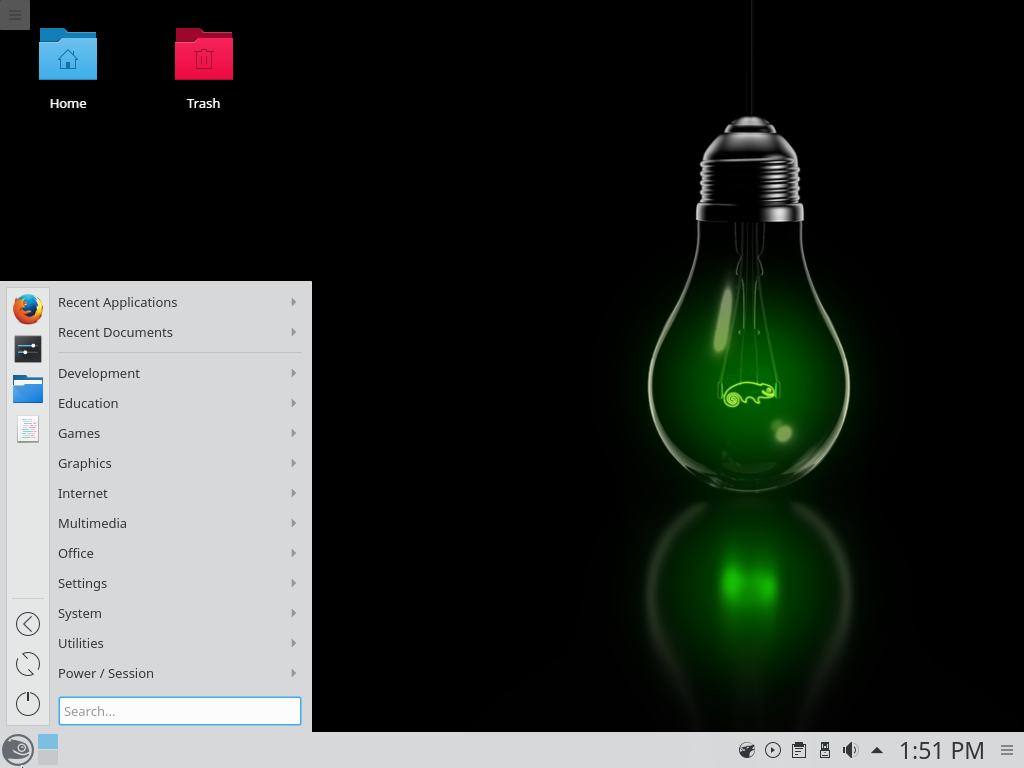
\includegraphics[height=7cm]{opensuse.png}
  \end{center}
\end{frame}

\begin{frame}{Fedora with GNOME -- GNOME is always almost same}
  \begin{center}
    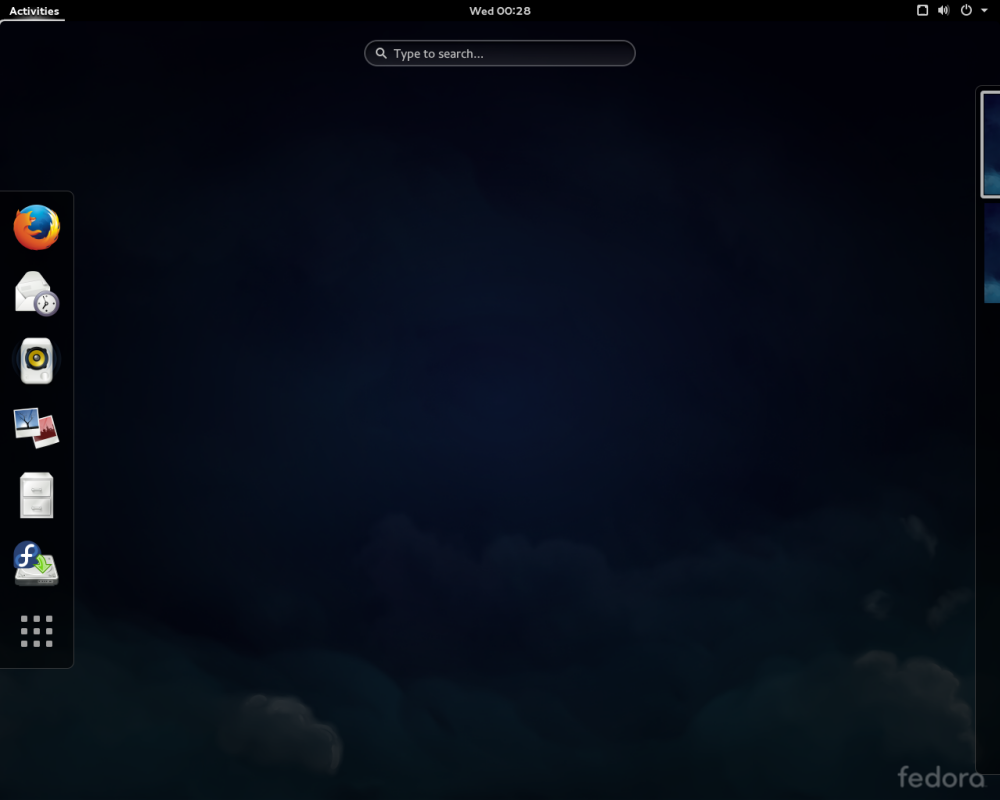
\includegraphics[height=7cm]{fedora.png}
  \end{center}
\end{frame}

\begin{frame}{Linux Mint with Cinnamon}
  \begin{center}
    
\includegraphics[height=7cm]{mint.png}
  \end{center}
\end{frame}

\begin{frame}{Debian with XFCE -- Xubuntu has more ``modern'' design}
  \begin{center}
    
\includegraphics[height=7cm]{debian.png}
  \end{center}
\end{frame}

\begin{frame}{How to try it?}
  \begin{itemize}
    \item Install it on some computer together with or instead of Windows
    \begin{itemize}
      \item If you can use whole disk, just boot from CD/USB and click ``Next''\ldots
      \item If you don't have whole disk, you need at least one (commonly more) disk partition(s) -- if you don't know how to manage them, ask someone skilled\ldots
    \end{itemize}
    \item Live CD/USB
    \begin{itemize}
      \item The most easy -- burn ISO image of CD from web of almost any Linux distribution or use for example \href{https://unetbootin.github.io/}{UNetbootin} to prepare bootable flash
      \item You only have to know how to boot from CD/USB (usually press \texttt{ESC}, \texttt{DEL}, \texttt{F2}, \texttt{F10}, \texttt{F12},~\ldots{ }when starting computer -- varies according to manufacturer)
    \end{itemize}
    \item Virtualization (slide~\ref{VBox})
    \begin{itemize}
      \item Requires relatively powerful computer (preferable Intel i5 or i7 and over 4~GB of RAM)
      \item Install virtual machine (probably the most easy is \href{https://www.virtualbox.org/}{VirtualBox}) -- allows install and run another operating system inside host as an ordinary application -- very easy and comfortable
    \end{itemize}
  \end{itemize}
\end{frame}

\subsection{Differences}

\begin{frame}{The Linux diversity\ldots}
  \begin{itemize}
    \item Try several distributions and just choose one you like\ldots
    \item Unless selecting among the most common, it doesn't matter much which one you pick up
    \item Which design do you like?
    \item Which distribution is your friend or colleague using? To have someone to ask for help\ldots
    \item You can change GUI (or its design) without change of distribution (it use to be highly configurable)
    \item Applications are still same -- no difference in Firefox across distributions -- keep your settings when changing distribution
    \item Everyone using Android is using Linux
    \item Special use -- \href{http://www.freenas.org/}{FreeNAS} for home as well as business file servers, \href{https://partedmagic.com/}{Parted Magic} and/or \href{https://www.system-rescue-cd.org/SystemRescueCd_Homepage}{SystemRescueCD} to repair broken system (disk failure) and save data,~\ldots
  \end{itemize}
\end{frame}

\begin{frame}{Differences among (common) Linux distributions}
  \begin{itemize}
    \item Design and colors ;-)
    \item Default GUI (other can be installed)
    \item Applications available right after installation
    \item Default settings (not much)
    \item Package management -- especially in command line
    \item Development model -- conservative or experimental, fast or slow
    \item Management of system services (how to start/stop certain services like database or web) -- not important for daily usage for most of users
    \item Sometimes in location of some system files -- also not important in daily usage of most of users
    \item Kernel is almost same, applications are same and used in same way
    \item Command line is almost same across Linux, and almost same as in other UNIX systems
  \end{itemize}
\end{frame}

\section{UN*X}

\begin{frame}[fragile]{Root vs. ``normal'' user}
  \begin{itemize}
    \item Root is administrator -- more than God -- can do anything
    \item Other users have limited permissions
    \begin{itemize}
      \item System users providing particular service (web server, database, networking service) are as restricted as possible to do the task -- security
      \item ``Human'' users don't have access to system files (at least not for modification), homes of users are separated
    \end{itemize}
  \end{itemize}
  \begin{bashcode}
    # Gain root privileges
    su # Requires root password (stay in current directory)
    su - # Requires root password (go to /root)
    su -c "some command" # Launch one command with root permissions
    su USER # Became USER (his password is required)
    sudo -i # For trusted users, became root (asks for user's password)
            # User has to be listed in /etc/sudoers
    sudo somecommand # Launch somecommand with root's privileges
                     # Can be restricted for particular commands
  \end{bashcode}
\end{frame}

\subsection{Disks and filesystems}

\begin{frame}{Short overview of hard disk layout}
  \begin{itemize}
    \item Physical disk (piece of hardware) has at least 1 partition -- division seen in Windows as ``disks'' (\texttt{C}, \texttt{D},~\ldots) and mounted directory in UNIX
    \item MBR -- older description of disk division, up to 4 primary partitions (OS typically requires at leas one to run), one can be extended and contain more partitions, disks up to 2 TB
    \item GPT -- newer, no relevant limits, requires UEFI (replacement of BIOS -- responsible for computer to start -- in newer computers)
    \item If unsure what to do, high probability to break it\ldots
    \item Blank new partition has to be formatted to desired file system according to use and target operating system
    \item Linux distributions have easy graphical tools to manage disk partitions (e.g. \href{http://gparted.org/}{GParted})
    \item Always have backup before such management!
  \end{itemize}
\end{frame}

\begin{frame}{Put together more disks}{Extend space and get higher data security}
  \label{LVMRAID}
  \begin{itemize}
    \item \href{https://en.wikipedia.org/wiki/RAID}{RAID} -- Redundant Array of Inexpensive/Independent Disks
    \item RAID~0 -- stripping, no redundancy, no security, speed up (two or more disks joined into one, files divided among disks)
    \item RAID~1 -- mirroring -- even number of disks of same size -- resulting capacity is half, very fast, secure
    \item RAID~5 -- at least three disks, one is used for parity control, little bit slower
    \item Combinations (RAID~10,~\ldots)
    \item \href{https://en.wikipedia.org/wiki/Logical_volume_management}{LVM} -- Logical Volume Management -- built over several partitions/disks -- seen by OS as one continuous space, can be dynamically managed
    \item Functionality of RAID and LVM (and more) is more or less covered by XFS and Btrfs (next slide)
  \end{itemize}
\end{frame}

\begin{frame}{File systems}
  \begin{center}
    \begin{footnotesize}
      \begin{tabular}{ccccccc}
	\textbf{FS name} & \begin{tabular}[x]{@{}c@{}}\textbf{Name}\\\textbf{length}\end{tabular} & \begin{tabular}[x]{@{}c@{}}\textbf{Characters}\\\textbf{in file name}\end{tabular} & \begin{tabular}[x]{@{}c@{}}\textbf{Path}\\\textbf{length}\end{tabular} & \textbf{File size} & \begin{tabular}[x]{@{}c@{}}\textbf{Partition}\\\textbf{size}\end{tabular} & \textbf{Systems}\\
	FAT32 & 255 & Unicode & No limit & 4 GiB & 2 TiB & Any\\
	exFAT & 255 & ? & No limit & 16 EiB & 64 ZiB & Any\\
	NTFS & 255 & Variable & Variable & 16 TiB & 16 EiB & \begin{tabular}[x]{@{}c@{}}Windows,\\read-write\\in UN*X\end{tabular}\\
	HFS+ & 255 & Unicode & ? & 8 EiB & 8 EiB & Mac OS\\
	ext4 & 255 & Any, not / & No limit & 16 TiB & 1 EiB & UN*X\\
	XFS & 255 & Any & No limit & 9 EiB & 9 EiB & UN*X\\
	Btrfs & 255 & Any & ? & 16 EiB & 16 EiB & UN*X
      \end{tabular}
    \end{footnotesize}
  \end{center}
  \begin{itemize}
    \item FAT32 (including extensions) is old-fashioned and not reliable FS
    \item NTFS, FAT do not support UNIX permissions, so they can't be used as system partition in Linux
    \item ext4, XFS and Btrfs are not accessible in Windows
    \item XFS and Btrfs are the most advanced FS in common use
  \end{itemize}
\end{frame}

\begin{frame}[allowframebreaks]{Creation and control of FS}
  \begin{itemize}
    \item All commands require root privileges
    \item \texttt{fdisk -l} lists disks and partitions
    \item To manage disk partitioning use \texttt{fdisk /dev/sdX} (doesn't support GPT very well yet) or \texttt{gdisk /dev/sdX}
    \item When hard drive is partitioned, partitions must be formatted
    \item Commands \texttt{mkfs.*} create various FS, common syntax is \texttt{mkfs.XXX -parameters /dev/sdXY}, where sdXY is particular disk partition
    \item Parameters can set label and various settings of behavior of the disk partition, check \texttt{man mkfs.XXX}
    \item To check FS for errors use \texttt{fsck.XXX /dev/sdXY} (according to respective FS)
    \begin{itemize}
      \item The filesystem must be unmounted when checking it
      \item XFS uses \texttt{xfs\_repair /dev/sdXY}
      \item Btrfs uses \texttt{btrfs check /dev/sdXY}, if it is unmountable, \texttt{btrfs-zero-log /dev/XY} use to help, last instance is \texttt{btrfs check --repair /dev/sdXY} (dangerous operation)
      \item If Btrfs is mountable, but there are various FS errors and/or performance issues, \texttt{btrfs scrub start -Bdf /mount/point}, \texttt{btrfs filesystem defragment -r -v /mount/point} and \texttt{btrfs balance start -v /mount/point} -- manual running can take long time and strongly slow down the computer
    \end{itemize}
    \item \texttt{tune2fs -parameters /dev/sdXY} can set various parameters to influence behavior of disk partition
    \item \texttt{hdparm -parameters /dev/sdX} can set advanced hardware parameters of hard drive
    \item The most convenient is using graphical tools available in all distributions\ldots
    \begin{itemize}
      \item In \href{https://doc.opensuse.org/documentation/leap/reference/html/book.opensuse.reference/cha.advdisk.html}{openSUSE there is YaST} administrative module -- from command line launch \texttt{yast --qt disk} for graphical or \texttt{yast disk} for text-based version
      \item All distributions have graphical tools like \href{http://gparted.org/}{GParted} where it is possible to comfortable manage disks
    \end{itemize}
    \item \texttt{df -h} shows available/occupied space on disks/partitions, but because of special features of Btrfs it doesn't show every time correct values for this FS -- it is better to use \texttt{btrfs filesystem df /mount/point} (\texttt{/mount/point} use to be the most commonly \texttt{/})
    \item On UNIX FS, defragmentation and another maintenance tasks use to be done in background when computer is idling -- unless there is at least $\sim$20\% of free space on the device, this is not any problem and there are no performance issues
  \end{itemize}
\end{frame}

\begin{frame}[fragile]{Another manipulations and information}
  \begin{itemize}
    \item \texttt{dd} is powerful, but potentially dangerous tool used to backup or write disks or partitions (commonly to create bootable USB media)
    \item If writing disk image to the disk (\texttt{sdX}), disk's partition table is discarded and the disk is covered by whatever is the ISO image
  \end{itemize}
  \begin{bashcode}
    dmesg # Recent entries in main system log - filter with grep, tail, ...
    dmesg | grep sd | tail # Get information about recently plugged media
    # dd produces physical copy of whole device - including empty space
    dd if=/dev/sdXY of=image.iso # Backups disk sdXY to imago.iso
    dd if=image.iso of=/dev/sdX # Used to write e.g. image of Linux live
                                # media to USB flash disk (Check sdXY!)
    lnav # Comfortably browse recent logs, quit by "q"
  \end{bashcode}
  \begin{itemize}
    \item If there are encrypted partitions, they can be accessed \texttt{/dev/mapper/\ldots}
    \item If LVM (slide~\ref{LVMRAID}) is used, see \texttt{lvscan} and \texttt{pvscan} to find correct location in \texttt{/dev/}
    \item Disks are also accessible through \texttt{/dev/disk/by-*}
  \end{itemize}
\end{frame}

\begin{frame}[fragile]{Mounting and unmounting disks and removable media}
  \begin{itemize}
    \item Mounting and unmounting of devices require root privileges
    \item In Linux, physical disks are named from \texttt{sda} to \texttt{sdz}, each disk has partitions (at least one) numbered from \texttt{1}, e.g. \texttt{sda1}, \texttt{sda2}, \texttt{sdb1},~\ldots{ }-- all are accessible in \texttt{/dev} directory (\texttt{/dev/sdc3},~\ldots)
    \item Target mount point must exist before mounting
  \end{itemize}
  \begin{bashcode}
    eject # Open CD/DVD drive
    mount # Which FS (disk partitions) are mounted
    findmnt # See mounted devices in tree-like structure
    mkdir /mnt/point # Directory must exist prior mounting into it
    # mount usually recognize FS of mounted device, if not, us -t FS_type
    mount /dev/sdXY /mount/directory # Mount disk sdXY to /mount/directory
    umount /dev/sdXY # Unmount disk sdXY
    umount /mount/directory # Unmount disk from /mount/directory
    # Mount CD/DVD ISO image file into directory /mnt/iso
    mount -t iso9660 -o loop file.iso /mnt/iso # See CD/DVD image content
  \end{bashcode}
\end{frame}

\subsection{Files and directories}

\begin{frame}[fragile]{File names}
  \begin{itemize}
    \item Linux allow \alert{any} character in file name, except \alert{slash} (\texttt{/}), so including anything on keyboard as well as line break (\alert{!}) -- be conservative\ldots
  \end{itemize}
  \begin{bashcode}
    mkdir My New Directory # Produces THREE directories (mkdir creates
                           # directories; spaces separate parameters)
                           # Solutions:
    mkdir "My New Directory" # (you can use simple quotes '...' as well) or
    mkdir My\ New\ Directory # "\" escapes following character
    rmdir My\ New\ Directory # Same problem and solution when removing it
    touch \* # Creates new empty file named just * (yes, asterisk)
    rm * # What would be removed? :-)
    rm \* # This works...
  \end{bashcode}
  \begin{itemize}
    \item Files and directories starting by \alert{dot} (\texttt{.}) are hidden by default (typically user settings and application data in user home)
  \end{itemize}
  \begin{bashcode}
    touch .hiddenfile # Let's make empty text file hidden by default
    ls # We will not see it (ls lists only "visible" files/directories)
    ls -a # We will see it ("-a" to see all - also hidden - files/dirs)
  \end{bashcode}
\end{frame}

\begin{frame}[allowframebreaks]{Directory structure in Linux}
  \begin{itemize}
    \item Similar is also in another UN*X systems
    \item Top directory ``\texttt{/}'' -- ``root''
    \item Everything else (including disks and network shares) are mounted in subdirectories (\texttt{/\ldots})
    \item \texttt{/bin} -- very basic command line utilities
    \item \texttt{/boot} -- bootloader responsible for start of system
    \item \texttt{/dev} -- devices -- representations of disks, CD, RAM, USB devices,~\ldots
    \item \alert{\texttt{/etc}} -- system configuration in plain text files -- edit them to change system-wide settings (read documentation and comments there)
    \item \alert{\texttt{/home}} -- users' homes
    \item \texttt{/lib}, \texttt{/lib64} -- basic system libraries (32 and 64bits)
    \item \texttt{/lost+found} -- feature of FS, after crash and recovery of FS, restored files are there
    \item \alert{\texttt{/media}} -- attached disks (USB flash,~\ldots) usually appear there (might be in \texttt{/var/run/media}) -- subdirectories are automatically created when device is plugged and disappears when unplugged
    \item \texttt{/mnt} -- usually manually mounted file systems (but can it can be mounted elsewhere)
    \item \texttt{/opt} -- optional, usually locally compiled software
    \item \texttt{/proc} -- dynamic information about system processes
    \item \texttt{/root} -- root's (admin's) home
    \item \texttt{/sbin} -- basic system utilities
    \item \texttt{/selinux} -- SELinux is security framework
    \item \texttt{/srv} -- FTP and WWW server data (can be in \texttt{/var/srv})
    \item \texttt{/sys} -- basic system
    \item \texttt{/tmp} -- temporary files -- users have private dynamically created spaces there
    \item \texttt{/usr} -- binaries (executable applications) and libraries of installed applications
    \item \alert{\texttt{/var}} -- data of most of applications and services, including e.g. database data, system logs,~\ldots
    \item \alert{\texttt{/windows}} -- if on dual boot, Windows disks are commonly mounted here
    \item Can be altered, modified
    \item Usually, work only in your home, anywhere else modify files only if you are absolutely sure what you are doing
    \item Normal user doesn't have permission to modify files outside his directory (with exception of plugged removable media)
    \item Try \texttt{man hier} for details
  \end{itemize}
\end{frame}

\begin{frame}{Configuration in /etc (examples)}
  \begin{itemize}
    \item Configuration of system services (servers,~\ldots) and behavior
    \begin{itemize}
      \item Apache web server, database, FTP server, networking, basic system settings,~\ldots
    \end{itemize}
    \item \texttt{cron*} -- cron automatically repeatedly runs tasks
    \item \texttt{fstab} -- description of FS mounted during startup
    \item \texttt{group} -- list of users and groups
    \item \texttt{passwd} -- basic settings of for users (home directory, default shell,~\ldots)
    \item \texttt{resolv.conf} --  DNS settings (part of basic networking)
    \item \texttt{shadow} -- users passwords in encrypted format
    \item \texttt{skel} -- basic directories and configuration for new users
    \item Much more\ldots
  \end{itemize}
\end{frame}

\begin{frame}[fragile]{Types of files}
  \begin{bashcode}
    ls -la ~
  \end{bashcode}
  \begin{itemize}
    \item Regular file -- ordinary file, marked by \texttt{-}
    \item Directory -- in UNIX special type of file, marked by \texttt{d}
    \item Symbolic link (symlink, ``soft link'') -- points to another place, marked by \texttt{l}, slide \ref{links}
    \item Hard link -- just another name for existing file, no special symbol, slide \ref{links}
    \item Block and character device -- in \texttt{/dev}, representations of devices (hard disks, terminals,~\ldots), marked by \texttt{b} or \texttt{c} respectively
    \item Named pipe -- pipe can be saved (by \texttt{mkfifo}), looks like a file, more at slide \ref{pipe}
    \item Socket -- for communication among processes, also bidirectional, available on network
  \end{itemize}
\end{frame}

\begin{frame}[fragile]{Links}
  \label{links}
  \begin{itemize}
    \item Soft links -- like links on the web -- short-cut to another place: \texttt{ln -s source target}
    \begin{itemize}
      \item When we delete link, nothing happens, when target, non-working link remains
    \end{itemize}
  \end{itemize}
  \begin{bashcode}
    ls -l bin/cinema5
    lrwxrwxrwx 1 vojta users 42 5. dub 2014 cinema5 -> # "l" marks link
      /home/vojta/bin/cinema5-0.2.1-beta/cinema5* # "->" points to target
  \end{bashcode}
  \begin{itemize}
    \item Hard links -- only second name for file already presented on the disk (available only for files): \texttt{ln source target}
  \end{itemize}
  \begin{bashcode}
    ln .bashrc .bashrcX
    ls -l .bash* # Numbers in first column show links pointing to it
                 # For directories - number of items, for files = 1
    -rw------- 1 vojta users 27298 21. led 16.43 .bash_history # One link
    -rw-r--r-- 2 vojta users  2707 29. lis 16.21 .bashrc # Same file as below
    -rw-r--r-- 2 vojta users  2707 29. lis 16.21 .bashrcX # Two links
  \end{bashcode}
\end{frame}

\subsection{Permissions}

\begin{frame}[fragile]{Owner and group}
  \begin{itemize}
    \item Every file has an owner and group -- for finer setting of rights
    \item Group can have just one member -- the user
    \item System usually shows names of groups and users, but important are IDs: GID and UID
    \item Commands \texttt{chown} requires root privileges
    \item Commands \texttt{chgrp} commonly requires root privileges -- user has to be member of particular group to be able to change ownership to it (if not, \texttt{root} most change group ownership)
    \item Information about users and groups and their IDs are in \texttt{/etc/group} and \texttt{/etc/passwd}
  \end{itemize}
  \begin{bashcode}
    ls -l # Shows also owner and group
    id # Display UID and GIDs of current user
    chown newowner:newgroup files # Change owner and group
    chown -R newowner files # Recursively (-R) change owner
    chgrp -R newgroup files # Recursively (-R) change group
  \end{bashcode}
\end{frame}

\begin{frame}{File and directory permissions}
  \begin{itemize}
    \item Combination of permissions to read/write/execute for user(owner)/group/others
  \end{itemize}
  \begin{center}
    \begin{tabular}{llll}
      \textbf{Permission} & \textbf{Number} & \textbf{Directory} & \textbf{File}\\
      r & 4 & Read content & Read content\\
      w & 2 & Write into it & Write into it\\
      x & 1 & Enter it & Launch application
    \end{tabular}
  \end{center}
  \begin{itemize}
    \item \texttt{rwxr-wr--} -- 3*3 characters for permissions for owner of the file/directory, group it is belonging to, and other users (\texttt{d} on beginning marks directories, \texttt{l} links, \texttt{+} ACL, slide \ref{acl})
    \item \texttt{764} -- same as above --- numbers for each role are summed -- first one is for owner, second for group and last for others
    \item Executable scripts and binaries \textbf{require} executable permission (\texttt{x})
  \end{itemize}
\end{frame}

\begin{frame}[fragile]{Permissions examples}
  \begin{bashcode}
    ls -l # Shows permissions, links, owner, group, size, date, name
    # Only owner can read and write the file; 600
    -rw-------   1 vojta users   38211 20. led 09.23 .bash_history
    # Owner can write read and write the file, others read; 644
    -rw-r--r--   1 vojta users    2707 29. lis 16.21 .bashrc
    # Owner can enter, read and write directory, others can read
    # and enter it; 755
    drwxr-xr-x  41 vojta users    4096 27. pro 09.55 bin
    # Only owner can read, write and enter the directory,
    # others nothing; 700
    drwx------  58 vojta users    4096 17. pro 15.45 .config
    # Link, everyone can do everything; 777
    lrwxrwxrwx   1 vojta users      37 20. led 09.33 .lyxpipe.in ->
      /tmp/kde-vojta/kilemj7d3E/.lyxpipe.in
    # Executable (application) - everyone can launch it, but only
    # owner can write into the file; 755
    -rwxr-xr-x   1 vojta users    2187 27. lis 13.10 strap.sh*
  \end{bashcode}
  \vfil
  \begin{itemize}
    \item Permission to ``write'' also means permission to \textbf{delete} it
  \end{itemize}
\end{frame}

\begin{frame}[fragile]{Check and modify permissions}
  \begin{bashcode}
    ls -l # Long list - file names and attributes
    ls -a # All, including hidden files (starting with dot)
    ls -F # Add on the end of name "/" for directories and "*"
          # for executable
    ls -h # Human readable size units (use with -l or -s)
    ls --color ## Coloured output
    ls -laFh --color # Combine any parameters you like
    chmod u/g/o/a+/-r/w/x FILE # For respective user/group/others/all adds/
                               # removes permission to read/write/execute
    chmod XYZ FILE # Instead of XYZ use number code of permission
    chmod -R # Recursive (including subdirectories)
    chmod +x script.sh # Make script.sh executable for everyone
    chmod o-r mydir # Remove read permission from others on mydir
    chmod 600 FILE1 FILE2 # Make both files readable and
                          # writable only by their owner
    chmod 000 FILE # No one can do anything - owner or root must add
                   # some permissions before any manipulation...
    chmod 777 * # All permissions for everyone on everything (no recursive)
  \end{bashcode}
\end{frame}

\begin{frame}[fragile]{Extending permissions -- ACL}{Access control list}
  \label{acl}
  \begin{itemize}
    \item By default, it is not possible to give specific permission to the user who is not owner, nor member of group owning the file
    \item In ext4 FS it has to be turned on manually (usually it is by default), it is part of XFS and Btrfs
    \item Command \texttt{getfacl} lists those extra permissions, \texttt{setfacl} sets
    \item When in use, ``basic'' tools listing permissions (e.g. \texttt{ls -l}, ACL in use is marked by \texttt{+} on the beginning of the line) sometimes do not show correct result
    \item Important especially in network environment with many users
    \item If intensively used, \texttt{ls -l} sometimes doesn't show correct permissions
  \end{itemize}
  \begin{bashcode}
    getfacl FILE # get ACL for FILE
    setfacl -m u/g:USER/GROUP:r/w/x FILE # Add for USER/GROUP r/w/x right
    setfacl -R ... # Recursive (including subdirectories)
    setfacl -b FILE # Remove all ACL from FILE
  \end{bashcode}
\end{frame}

\begin{frame}{Set default permissions for new files}
  \begin{itemize}
    \item \texttt{umask} sets implicit permissions for newly created files for user
    \item Syntax is similar to \texttt{chmod}, but reverse (e.g. \texttt{027} keeps all rights for owner, for group only reading and nothing for others)
    \begin{itemize}
      \item \texttt{umask} number \textbf{removes} certain permissions
    \end{itemize}
    \item \texttt{umask 027} (or other number) is typically set in file \texttt{$\sim$/.bashrc}
    \begin{itemize}
      \item \texttt{$\sim$} means user's home directory
      \item \texttt{.bashrc} is user's configuration for BASH
    \end{itemize}
    \item Typically used in network environment
    \item Set with care -- new permissions will have plenty of consequences -- different are typically needed for web pages, private files, shared files,~\ldots
    \item \texttt{umask} work recursively for all new files in user home directory -- it is not possible to set new implicit rules for particular directory
  \end{itemize}
\end{frame}

\begin{frame}[fragile]{Other permissions}
  \begin{itemize}
    \item \texttt{sticky bit} -- new directory/file in shared directory (where everyone can write) will be deletable only by owner (typically in \texttt{/tmp})
  \end{itemize}
  \begin{bashcode}
    chmod +t somedirectory
    ls -la /
    drwxrwxrwt 22 root root 800 21. led 18.20 tmp # "t" marks it
  \end{bashcode}
  \begin{itemize}
    \item \texttt{setgid} -- application can have root permission even it was launched by normal user
  \end{itemize}
  \begin{bashcode}
    chmod u+s someapplication
    ls -al /bin/passwd
    -rwsr-xr-x 1 root shadow 51200 25. zář 08.38 /usr/bin/passwd # Note "s"
  \end{bashcode}
  \begin{itemize}
    \item \texttt{chattr} -- change of advanced attributes on Linux FS
    \item Mostly, there is no need to modify them
  \end{itemize}
  \begin{bashcode}
    chattr -RVf -+=aAcCdDeijsStTu files
    man chattr # See explanation of attributes
    lsattr # List extended attributes
  \end{bashcode}
\end{frame}

\subsection{Text}

\begin{frame}{It \textbf{is} important to select \textbf{good} text editor\ldots}
  \begin{center}
    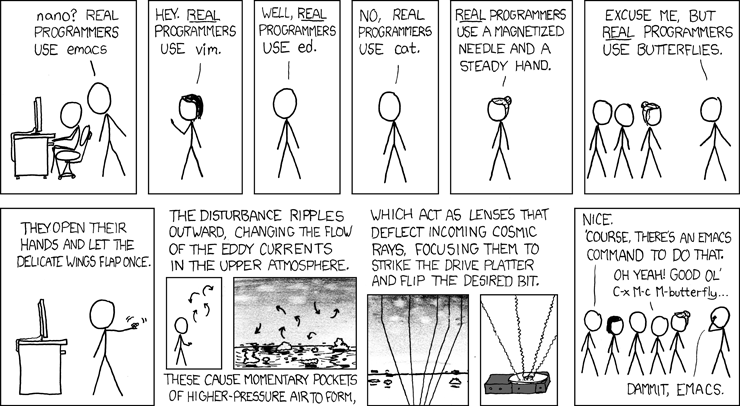
\includegraphics[width=\textwidth-1cm]{real_programmers.png}
  \end{center}
  \begin{flushright}
    \url{https://xkcd.com/378/}
  \end{flushright}
\end{frame}

\begin{frame}{Importance of good text editor}{Can your text editor\ldots ?}
  \label{editors}
  \begin{multicols}{2}
    \begin{itemize}
      \item Show syntax highlight
      \item Show line numbers
      \item Show space between brackets
      \item Open any encoding and EOL
      \item Fold source code
      \item Show line breaks
      \item Mark lines
      \item Open multiple files
      \item Advanced search and replace
      \item Use regular expressions
      \item Make projects, add notes
      \item Use command line
      \item Check spelling
      \item Debug source code
    \end{itemize}
  \end{multicols}
  \begin{multicols}{4}
    \begin{itemize}
      \item \href{http://kate-editor.org/}{Kate}
      \item \href{https://www.kde.org/applications/utilities/kwrite/}{KWrite}
      \item \href{http://www.vim.org/}{Vim}
      \item \href{https://en.wikipedia.org/wiki/Emacs}{GNU Emacs}
      \item \href{https://www.geany.org/}{Geany}
      \item \href{http://bluefish.openoffice.nl/index.html}{Bluefish}
      \item \href{https://wiki.gnome.org/Apps/Gedit}{Gedit}
      \item \href{https://notepad-plus-plus.org/}{Notepad++}
      \item \href{https://www.sublimetext.com/}{Sublime}
      \item \href{https://atom.io/}{Atom}
      \item \href{https://www.nano-editor.org/}{Nano}
      \item And \href{https://en.wikipedia.org/wiki/List_of_text_editors}{more}\ldots
    \end{itemize}
  \end{multicols}
\end{frame}

\begin{frame}{Text and text -- differences among operating systems}
  \begin{itemize}
    \item Windows and UNIX have different internal symbol for end of line (new line) -- EOL
    \begin{itemize}
      \item UNIX: LF (\texttt{\textbackslash n})
      \item Windows/DOS: CR+LF (\texttt{\textbackslash r\textbackslash n})
      \item Mac v. < 9: CR (\texttt{\textbackslash r}) (Mac up to 9 wasn't UN*X, since OS~X it is)
    \end{itemize}
    \item Good text editor can open correctly any EOL, but for example execution of script written in Windows will probably fail on Linux
    \item Different systems use different encoding
    \begin{itemize}
      \item UNIX: mainly UTF-8 (unicode, universal)
      \item Windows: win-cp-125X (variants according to region)
      \item Older UNIX: ISO-8859-X (variants according to region)
      \item Other much less common types
    \end{itemize}
    \item Text editors can usually open any encoding, but auto detection commonly fails -- set it manually
  \end{itemize}
\end{frame}

\begin{frame}[fragile]{Converting the text}{Prevent bad display and weird errors when launching scripts}
  \begin{bashcode}
    unix2dos textfile # Convert text file from UNIX to Windows EOL
    unix2mac textfile # Convert text file from UNIX to old Mac EOL
    dos2unix textfile # Convert text file from Windows to UNIX EOL
    mac2unix textfile # Convert text file from old Mac to UNIX EOL
    unix2dos --help # More information about usage, include encodings
    # Converts encoding of input file (ISO-8859-2) to outfile in UTF-8
    iconv -f ISO-8859-2 -t UTF-8 infile.txt > outfile.txt
    iconv -l # List of available encodings to convert
    iconv --help # More information about usage
    recode CP1250..UTF-8 textfile # Convert encoding from CP-1250 to UTF-8
    recode ../CR-LF textfile # Convert EOL from UNIX to Windows
    recode -l # List of available encodings to convert
    recode --help # More information about usage
  \end{bashcode}
  \begin{itemize}
    \item Mac OS~X mostly uses same encoding and EOL as Linux (and rest of UNIX world), so there are no problems with compatibility
    \item Launching of bash script written on Windows on Linux/Mac OS~X will probably fail (because of different EOL)
  \end{itemize}
\end{frame}

\subsection{Variables}

\begin{frame}{Variables}
  \begin{itemize}
    \item Variables contain various information (where to look for the executable programs, name of the computer, user settings,~\ldots)
    \item Can be local (within a script for some temporal purpose) or global -- available for all processes
    \item Names commonly written in CAPITALS (just a costume)
    \item Popular and useful variables
    \begin{itemize}
      \item \texttt{HOME} -- location of user's home directory
      \item \texttt{HOSTNAME} -- network name of the computer
      \item \texttt{LANG} -- language settings, encoding, similarly variables \texttt{LC\_*}
      \item \texttt{PATH} -- paths where to look for applications -- all applications have to be in \texttt{PATH} or called directly
      \item \texttt{SHELL} -- shell in use (bash or something else)
      \item \texttt{USER} -- user name
      \item And many more, commonly specific for particular server
    \end{itemize}
  \end{itemize}
\end{frame}

\begin{frame}[fragile]{Work with variables}
  \begin{bashcode}
    printenv # Get all exported variables and their values
    export -p # Get all exported variables and their values
    echo $VARIABLENAME # Get value of particular variable
    echo $PATH # Get path where to look for applications
    VARIABLE='variablevalue' # Set new variable and its value
                             # Or replace existing variable by new value
    export EDITOR=/usr/bin/vim # Set new default text editor
    export PATH=$PATH:~/bin # Extend PATH -- add /home/$USER/bin
                            # Take existing PATH and add new values
                            # separated by ":"
    export GREP_OPTIONS='--color=auto' # Coloured grep
    unset VARIABLENAME # Drop variable and its value
  \end{bashcode}
  \begin{itemize}
    \item Exported variables will be lost when logging off
    \item To make variables permanent, add \texttt{export} commands into \texttt{$\sim$/.profile} or \texttt{$\sim$/.bash\_profile}, or \texttt{$\sim$/.bashrc} (according to shell and its settings)
    \item ``\texttt{$\sim$}'' means home directory
  \end{itemize}
\end{frame}

\begin{frame}[fragile]{The PATH variable}
  \begin{itemize}
    \item Lists directories (separated by colon \texttt{:}) where the current shell searches for commands
    \item If some software is installed outside standard locations, the user must specify the full path (or update the \texttt{\$PATH})
    \item In case there are two commands with the same name (e.g. \texttt{/bin/somecommand} and \texttt{/usr/bin/somecommand}), the order of directories in \texttt{\$PATH} matters -- the first occurrence is used, any possible later ignored
  \end{itemize}
  \begin{bashcode}
    # See the $PATH variable
    echo $PATH # Sample output is on the next line:
    /home/$USER/bin:/usr/local/bin:/usr/bin:/bin:/opt/bin:/sbin:/usr/sbin
    # Adding new directory to $PATH
    export PATH=$PATH:/some/new/directory # Ensure to add original $PATH
    # Do not do it in the following way - it would overwrite $PATH, and
    #   there would be only the new directory (not the original content)!
    export PATH=/some/new/directory # Wrong! Old $PATH is missing!
  \end{bashcode}
\end{frame}

\begin{frame}[fragile]{Reading variables from command line and as output of another commands}{This is especially useful in scripting to read input from users or from another commands}
  \begin{bashcode}
    # Reading variable from user's input from command line
    # (some interactive script interacting with the user)
    read X # We will read new variable from input (do not use "$" here)
    10 # Type any value and press Enter
    echo $X # Get value of the variable
    10 # It works
    # Following two commands are same and lead to same result
    X=`command` # Set as variable output of command
    X=$(command) # Set as variable output of command
    echo $X # X will contain output of command
    # "command" from previous lines can be e.g.
    cat somefile.txt # Read content of somefile.txt
    expr 1 + $X # Sum of 1 and variable $X
    WORKDIR=`pwd`# Save current directory into variable
    ls -1 | head -n 1 # First file/directory in the current directory
    unset X # Destroy this variable
  \end{bashcode}
\end{frame}

\begin{frame}[fragile]{Variables and quotes and more}
  \begin{bashcode}
    A=abcdef # Set new variable (no special characters allowed)
    echo $A # See variable's content
    abcdef # It works
    echo '$A' # Single quotes preserve literal value
    $A # We see variable's name, not its content
    echo "$A" # Double quotes preserve literal value, except $, `, \
    abcdef # This also works
    echo `$A` # Text between back ticks is evaluated and launched
    abcdef: command not found # There is no command "abcdef"...
    echo "Hi, dear $USER" # Compare this and following command...
    echo 'Hi, dear $USER' # Single quotes do not evaluate variables
  \end{bashcode}
  \begin{itemize}
    \item \alert{\texttt{\textdollar}} marks variables
    \item \alert{\texttt{\textbackslash}} escapes following character -- it will not have its special meaning (space to separate arguments,~\ldots)
    \item If variable is going to contain any special character (\texttt{?}, \texttt{.}, \texttt{*},~\ldots), the value must be quoted -- \texttt{"\ldots"} allow escaping of special character or inclusion of another variables, \texttt{'\ldots'} keeps absolutely literal value
  \end{itemize}
\end{frame}

\begin{frame}[fragile]{How quotes influence reading of variable content}
  \begin{bashcode}
    A=abcde # OK
    echo $A # abcde
    B=abcd$e # The content will be "abcde + $e" or "abcd" (if $e is missing)
    echo $B # abcd
    C=abcd\$e # \ escapes next character - it is loosing its special meaning
    echo $C # abcd$e
    D='abcd$e' # '...' keep literal value of the content
    echo $D # abcd$e
    # Next command breaks shell - incomplete quotes " - pres then Ctrl+C
    E=ab"cde # The variable should contain incomplete quotes ", it fails
    echo $E # Nothing - empty
    F=ab\"cde # \ escapes next character - it is loosing its special meaning
    echo $F # ab"cde
    G='ab"cde' # '...' keep literal value of the content
    echo $G # ab"cde
    H=abc`echo $USER`de # See $USER to see what will be inserted into `...`
    echo $H # abcvojtade # To add output of command into the variable
    I='...' # Needed if $I should contain spaces, quotes, `, $, ...
  \end{bashcode}
\end{frame}

\section{Command line}

\begin{frame}{Launching commands and scripts}
  \begin{itemize}
    \item Parameters of commands are separated by space and preceded by one or two minus(es)
    \item Parameter \texttt{-h} or \texttt{--help} usually gives help for particular command
    \item Getting help with \texttt{man} command
    \begin{itemize}
      \item \texttt{man somecommand}
      \item Arrows to list up and down, \texttt{q} to quit
      \item Type \texttt{/} and type text and hit Enter to search -- next hit by \texttt{n}, quit search by ESC (twice)
      \item Command \texttt{info} more advanced -- type \texttt{?} for help
    \end{itemize}
    \item Parameters can be combined, order doesn't matter (same variants: \texttt{ls -la}; \texttt{ls -al}; \texttt{ls -a -l}; \texttt{ls -l -a})
    \item ``Long'' parameters (\texttt{--XXX}) must stay separated
    \item Commands must be in PATH -- actual directory isn't in PATH
    \begin{itemize}
      \item If the script is is current directory, use \texttt{./script.sh} or full path
    \end{itemize}
    \item Custom scripts must have execute permission (\texttt{chmod +x script.sh})
  \end{itemize}
\end{frame}

\begin{frame}[fragile]{Login to remote server}{SSH -- secure shell -- encrypted connection}
\begin{multicols}{2}
  \begin{bashcode}
    ssh remoteUser@remote.server.cz
    # When logging first time, check
    # and confirm fingerprint key
    yes # And press Enter
    # Type remote user's password
    # (nothing is shown when typing)
    # Confirm by Enter
  \end{bashcode}
  \begin{itemize}
    \item Our toy server: user names from \texttt{u01} to \texttt{u30}
  \end{itemize}
  \begin{bashcode}
    ssh uXY@vyuka.natur.cuni.cz
  \end{bashcode}
  \begin{itemize}
    \item If fingerprint key changes, ssh complains a lot -- possible \href{https://en.wikipedia.org/wiki/Man-in-the-middle_attack}{man in the middle attack}
    \item From Windows use \href{http://www.putty.org/}{Putty}
  \end{itemize}
  \begin{center}
    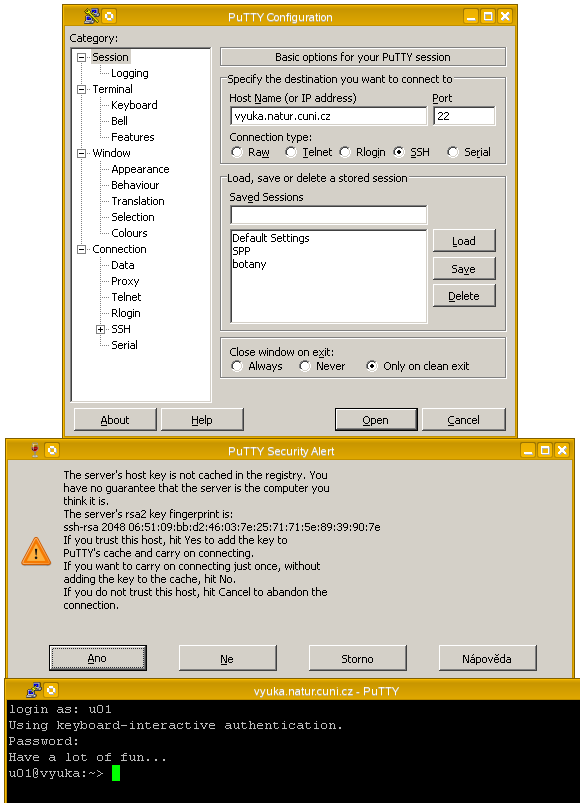
\includegraphics[height=6cm]{putty.png}
  \end{center}
\end{multicols}
\end{frame}

\begin{frame}{Screen}{Split terminal or keep task running after logging off}
  \begin{itemize}
    \item When you log off or network connection is broken, running tasks for particular terminal usually crash
    \item Sometimes number of connections is limited
    \item \texttt{screen} is solution -- virtual terminals
    \item Launch \texttt{screen} to start new screen terminal, read some info, confirm by \textbf{Space key} or \textbf{Enter}
    \item To detach from the screen press \texttt{Ctrl+A, D} -- screen is still running in background -- you can even log off
    \item To return back to running screen use \texttt{screen -r} -- if only one screen is running, you get back to it
    \item If more screens are running, use \texttt{screen -r 1234} (the number is seen from \texttt{screen -r})
    \item To cancel running screen press \texttt{Ctrl+D} (or type \texttt{exit} or \texttt{logout})
  \end{itemize}
\end{frame}

\subsection{BASH and others}

\begin{frame}{The shell}
  \begin{itemize}
    \item Many names, many ways how to get it, still the same thing
    \item Fish -- friendly interactive shell -- the command line interface
    \item Terminal (console)
    \begin{itemize}
      \item Originally machine used for connection to remote server
      \item System uses old fashioned terminal for inner purposes
      \begin{itemize}
	\item From GUI available using \texttt{Ctrl+Alt+F1} to \texttt{F12}
	\item Changing terminals using \texttt{Alt+F1} to \texttt{F12}
	\item Return back to GUI using \texttt{Alt+F7}
	\item Some are used for log outputs etc.
      \end{itemize}
      \item Nowadays used ``indirectly'' with special applications (``emulators'')
    \end{itemize}
    \item Terminal emulator
    \begin{itemize}
      \item Application used to get the ``terminal'' and work in command line
      \item Every GUI has some -- \href{https://konsole.kde.org/}{Konsole}, \href{https://yakuake.kde.org/}{Yakuake}, \href{http://invisible-island.net/xterm/}{XTerm}, \href{https://wiki.gnome.org/Apps/Terminal}{Gnome Terminal}, \href{http://guake.org/}{Guake}, \href{http://docs.xfce.org/apps/terminal/start}{XFCE Terminal}, \href{https://wiki.lxde.org/en/LXTerminal}{LxTerminal},~\ldots
      \item Commonly allow appearance customization -- font, colors, background, style of notifications,~\ldots
      \item Launch as many copies as you need (usually allow tabs for easier work)
    \end{itemize}
  \end{itemize}
\end{frame}

\begin{frame}{BASH and others}
  \begin{itemize}
    \item Shell (\textbf{sh}) -- feature rich scripting programming language -- general specification, several variants
    \item So called POSIX shell -- Portable Operating System Interface -- transferable among hardware platforms (and UNIX variants)
    \item \textbf{Interpreter of our commands inserted into command line}
    \item \textbf{BASH} -- Bourne again shell
    \begin{itemize}
      \item Probably the most common shell, based on original sh, respecting original specification, adding new features
      \item We will use it
    \end{itemize}
    \item Other variants: \textbf{csh} (syntax influenced by C), \textbf{ksh} (younger, backward compatible with bash), \textbf{zsh} (extended bash), \textbf{ash} (mainly in BSD)
    \item There are some differences in syntax and features
    \item Language suitable for easy scripting and system tasks, not for ``big'' programming, neither for graphical applications
  \end{itemize}
\end{frame}

\begin{frame}{Nice BASH features for easier work (selection)}
  \begin{itemize}
    \item Arrows up and down list in the history of commands
    \item List whole history by command \texttt{history}
    \item \texttt{Ctrl+R} -- reverse search in history -- type to search last command containing typed characters
    \item \texttt{TAB} -- list command and files starting by typed characters
    \item \texttt{Home}/\texttt{End} -- go to beginning/end of the line
    \item \texttt{Ctrl+L} -- clear screen (like \texttt{clear} command)
    \item \texttt{Ctrl+Shift+C}/\texttt{V} -- copy/paste the text
    \item \texttt{Ctrl+C} -- cancel running task
    \item \texttt{Ctrl+D} -- log out (like commands \texttt{exit} or \texttt{logout})
    \item \texttt{Ctrl+U} -- move text before cursor into clipboard
    \item \texttt{Ctrl+K} -- move text after cursor into clipboard
    \item \texttt{Ctrl+left/right arrow} -- skip words
    \item \texttt{Ctrl+T} -- flip current and left character
    \item \texttt{Ctrl+X+E} -- start text editor in current directory
  \end{itemize}
\end{frame}

\begin{frame}{Places to store BASH settings}
  \begin{itemize}
    \item \texttt{/etc/bash.bashrc} -- System wide BASH settings -- can be overridden by user's configuration
    \item \texttt{$\sim$/.bashrc} -- File is loaded each time user creates new session (typically opens new terminal window)
    \item \texttt{$\sim$/.bash\_profile} -- Used specifically (not in every system) when user is using remote connection (SSH)
    \item \texttt{/etc/profile} -- System wide profile file -- can be overridden by user's configuration
    \item \texttt{$\sim$/.profile} -- Settings loaded when user logs-in (mainly for language settings), sometimes used by remote connections
    \item \alert{Note:} BASH scripts are non-interactive shells -- they do not read settings above -- there are no aliases,~\ldots{ }but they inherit some settings (PATH, language,~\ldots) and they can read global variables
  \end{itemize}
\end{frame}

\begin{frame}[fragile]{BASH settings}{Write them into BASH configuration file}
  \begin{itemize}
    \item In any text editor open \texttt{$\sim$/.bashrc} and edit it
    \item Behavior of BASH can be set to fit user's needs
    \item Terminal emulators allow to set custom fonts and colors,~\ldots
  \end{itemize}
  \begin{bashcode}
    # More colors for outputs
    eval "`dircolors -b`"
    # Ignore repeated entries in bash history (stored in ~/.bash_history)
    HISTCONTROL='ignoreboth'
    # Maximal length (number of lines) of bash history (~/.bash_history)
    HISTFILESIZE='100000'
    # Following two settings save history from multiple terminals
    # Normally, only history from last time opened terminal is kept
    shopt -s histappend # Append to history, don't overwrite it
    # Save and reload the history after each command finishes
    export PROMPT_COMMAND="history -a; history -c; history -r;
      $PROMPT_COMMAND" # Note recursive behaviour of $PROMPT_COMMAND
  \end{bashcode}
\end{frame}

\begin{frame}[fragile]{Aliases and BASH settings}{Alias is short cut -- instead of very long command write short alias}
  \begin{bashcode}
    # Define new alias
    alias ll="ls -l"
    # Since now, instead of "ls -l" we can write just "ll"
    # To make the change above permanent, write it into ~/.profile or
    # ~/.bash_profile or ~/.bashrc and reload the configuration
    source ~/.bashrc # to reload BASH settings
                     # or "source" the file you modified
    # If there are many aliases, they can be stored e.g. in ~/.alias
    test -s ~/.alias && . ~/.alias || true # Check for extra alias file
    # Popular aliases
    alias ls="ls --color=auto" # Make output of ls colored
    alias l="ls -la" # Long list (add details) with hidden files
    # Popular settings in ~/.bashrc (influencing bash, not other shells)
    alias grep='grep --colour=always' # Enable color in grep
    # Always human readable output of df (disk free)
    alias df='df -h'
    # Add aliases pointing to software installed outside PATH, ...
  \end{bashcode}
\end{frame}

\begin{frame}{BASH globbing and wildcards}
  \label{globbing}
  \begin{itemize}
    \item BASH itself doesn't recognize regular expressions -- it's wildcards have some of functions of regular expressions (from slide~\ref{regexp}) and can look similarly, but behave differently! Do not confuse!
    \item \texttt{?} -- Replaces any single character
    \item \texttt{*} -- Replaces any number of any characters (\texttt{ls a*} lists all files starting with ``a'')
    \item \texttt{[]} -- Range or a list -- \texttt{[abcdef]} and \texttt{[a-f]} are same
    \item \texttt{[!\ldots]} -- Reverse previous case (\texttt{!}) -- any character except those listed
    \item \texttt{\{\}} -- Expansion (terms inside are separated by commas \texttt{,}) -- all possible combinations (see next slide for examples)
    \item \texttt{\textbackslash} -- Escapes following character and it doesn't have its special meaning (e.g. \texttt{\textbackslash *} means asterisk \texttt{*} and not ``any number of characters'')
    \item For details see \texttt{man 7 glob} and \texttt{man 7 regex}
  \end{itemize}
\end{frame}

\begin{frame}[fragile]{Brace expansion and quotes}
  \begin{bashcode}
    echo a{p,c,d,b}e # ape ace ade abe - all combinations
    echo {a,b,c}{d,e,f} # ad ae af bd be bf cd ce cf - all combinations
    ls *.{jpg,jpeg,png} # expansion to *.jpg *.jpeg *.png, same as
    ls *.jpg *.jpeg *.png
  \end{bashcode}
  \begin{itemize}
    \item Text in single quotes (\texttt{'\ldots'}) preserves the literal value of each character within the quotes
    \item Tex tin double quotes (\texttt{"\ldots"}) preserves the literal value of all characters within the quotes, with the exception of dollar (\texttt{\textdollar}), back tick (\texttt{\textasciigrave}) and back slash (\texttt{\textbackslash})
    \item A double quote may be quoted within double quotes by preceding it with a backslash
    \item Text between back ticks (\texttt{\textasciigrave\ldots\textasciigrave}) will be evaluated and then used as command or argument
  \end{itemize}
\end{frame}

\begin{frame}[fragile]{Expressions}
  \begin{bashcode}
    # Many operands have special meaning in BASH - must be escaped
    echo `expr 1 '<' 2` # Is 1 smaller than 2? TRUE (1)
    echo `expr 1 '>' 2` # Is 2 smaller than 1? FALSE (0)
    echo `expr 5 '%' 2` # What remains after aritmetic division
    echo `expr 1 '&' 0` # If both arguments non-empty and not 0, then 1
    x=`expr 1 '+' 6` # Result will be in $x
    echo $x
    x=1 # Set x to 1
    y=$x+1 # Will this add 1? Why?
    echo $y # See result
    y=`expr $x + 1` # This will work - note ` and space around +
    echo $y # Result
    echo `expr length "MetaCentrum and Linux"` # Get length of chain
    # String of 5 characters starting at position 10 of the text
    echo `expr substr "MetaCentrum and Linux" 10 5`
    # Does 1st chain contain 2nd chain (how long)? Get position of first hit
    echo `expr index "GNU Linux" "Linux"` # If no overlap, return value is 0
  \end{bashcode}
  \begin{itemize}
    \item \texttt{expr} works with various operands (see \texttt{man expr})
  \end{itemize}
\end{frame}

\subsection{Chaining}

\begin{frame}{Chaining commands}
  \begin{itemize}
    \item \alert{\texttt{\&}} -- command will be launched in background, terminal is available for next typing: \texttt{firefox \&} (when launching graphical application, hit \textbf{Enter} afterward if there is no active command line prompt)
    \item \alert{\texttt{\&\&}} -- second command is launched only when first command exits without error (exits with status \texttt{0}): \texttt{mkdir NewDir \&\& cd NewDir}
    \item \alert{\texttt{;}} -- second command is launched regardless exit status of the first one: \texttt{kshfskcbd; hostname}
    \item \alert{\texttt{\textbraceleft\ldots\textbraceright}} -- commands within curl brackets are launched as one block
    \item \alert{\texttt{||}} -- second command is launched when first command fails (has non zero exit status):\\\texttt{cd newdir || \textbraceleft~mkdir newdir \&\& cd newdir; \textbraceright}
    \item \alert{\texttt{|}} -- pipe -- redirects standard output of one command into standard input of second command: compare \texttt{mount} and \texttt{mount | column -t}
    \item Behavior in shells other than bash might be little bit different
  \end{itemize}
\end{frame}

\begin{frame}{Redirects and pipes}
  \label{pipe}
  \begin{itemize}
    \item \texttt{/dev/null} -- ``black hole''
    \begin{itemize}
      \item Can discard anything
      \item Discard only errors (note``2''): \texttt{command 2\textgreater~/dev/null}
    \end{itemize}
    \item \texttt{/dev/stdin} -- standard input
    \begin{itemize}
      \item Typically keyboard
      \item In case application reads files, not from standard input: \texttt{echo "Žluťoučký kůň úpěl" | iconv -f utf-8 -t cp1250 /dev/stdin}
    \end{itemize}
    \item \texttt{/dev/stdout} -- standard output
    \begin{itemize}
      \item Typically screen, commonly redirected into file
      \item We wish to see errors which would be discarded otherwise: \texttt{command 2\textgreater~/dev/stdout}
    \end{itemize}
    \item \texttt{/dev/stderr} -- standard error output
    \begin{itemize}
      \item Typically screen or log file
      \item Right place to send errors to: \texttt{echo "error" > /dev/stderr}
    \end{itemize}
    \item \texttt{|} -- pipe -- basic redirecting method -- standard output of one command to standard input of another command
  \end{itemize}
\end{frame}

\begin{frame}[fragile]{Standard input and output and redirects}
  \begin{itemize}
    \item Standard input (\texttt{stdin}) is standard place where software takes input (keyboard and terminal) and writes results to standard output (\texttt{stdout}) -- typically monitor
    \item Standard error output (\texttt{stderr}) is target of error messages -- typically also monitor (but can be log file or so)
    \item \alert{\texttt{\textgreater}} redirects output into new place (file, device, another command,~\ldots)
  \end{itemize}
  \begin{bashcode}
    cat /etc/group # Print whole file /etc/group
    grep users /etc/group > users # Extract from /etc/group lines containing
                                  # "users" and write output into new file
    cat users # See result
  \end{bashcode}
  \begin{itemize}
    \item \alert{\texttt{\textgreater\textgreater}} adds output to the end of the file (\texttt{\textgreater} rewrites target file)
  \end{itemize}
  \begin{bashcode}
    grep root /etc/group >> users # Add new information into existing file
    cat users # See result
  \end{bashcode}
\end{frame}

\begin{frame}[fragile]{Redirects of standard input and output}
  \begin{bashcode}
    # Write directory listing into text file
    # If file directory_listing.txt exists, will be overwritten
    ls -la > directory_listing.txt
    cat directory_listing.txt # See result (same as running "ls -la")
    # If file directory_listing.txt exists, new content will be appended
    ls -la >> directory_listing.txt
    cat directory_listing.txt # See result
    # Add error output to the end of standard output file
    # Note: In the examples below command "commandX" does not exist -
    # it produces error "command not found" to be recorded by the log
    # and because of redirect, the error is not shown in the terminal.
    command >> outputfile.log 2>&1 # Example:
    { commandX; ls; } >> outputfile 2>&1
    cat outputfile # See result
    # Add error output to the error log text file
    command >> outputfile.log 2>error.log # Example:
    { commandX; ls; } >> outputfile.txt 2>error.log
    cat outputfile.txt # See results
    cat error.log # See results
  \end{bashcode}
\end{frame}

\subsection{Information and processes}

\begin{frame}[fragile]{Which system are we using?}
  \begin{bashcode}
    uname -a # Information about Linux kernel (version, ...)
    lsb_release -a # Information about Linux distribution release
    cat /etc/os-release # Similar to above command
    lscpu # Information about CPU
    cat /proc/cpuinfo # Raw list of information about CPU
    lsusb # List of devices on USB
    lspci # List of PCI devices (graphic card, network card, ...)
    lshw # Complete list of hardware
    lshw -C memory # Information about RAM
    hwinfo # Complete list of hardware
    hwinfo --network # Information about network devices
    free -h # Available memory (RAM) and swap, -h for nice units
    df -h # Free space on disk partitions, -h for nice units
    lsmod # List loaded kernel modules
    uptime # How long is the system running, number of users, average load
    date # Date and time - plenty of options for formatting
    mount # Information about mounted file systems
    findmnt # Display mounted devices in tree structure
  \end{bashcode}
\end{frame}

\begin{frame}[fragile]{Processes -- every running program has its own process ID}
  \begin{bashcode}
    htop # Nice listing of processes (better version of top), quit using "q"
    pstree # See running processes with child processes, recursively
    pgrep application # Return PID (process ID) of application
    ps # processes related to actual terminal
    ps x # All user's processes
    ps aux # All processes
    # kill (terminate) process by name or process ID (PID)
    ps aux | grep geany # Find which PID has application to terminate
    # This is the application - its PID we need
    vojta 14639 9.3 0.8 2828512 134816 ?   Sl 16:12 0:01 /usr/bin/geany
    # This is the previous "ps aux | grep geany" command (last column)
    vojta 14769 0.0 0.0   9440  1628 pts/0 S+ 16:12 0:00 grep geany
    kill -SIGTERM 14639 # SIGTERM is "nice" termination, SIGKILL "brutal"
    killall -SIGTERM geany # Select by name (more processes with same name)
    # nice - how much resources will task use: from -20 (high priority - not
    # "nice" process) to +19 (low priority - very "nice" process), default 0
    nice -n 7 hard_task.sh # set priority 7 for newly launched task
    renice 15 16302 # Change priority of PID 16302 to 15
    sudo renice 15 16302 -u USER # Change priority of USER's process
  \end{bashcode}
\end{frame}

\begin{frame}[fragile]{Users}
  \begin{bashcode}
    whoami # What is my user name
    id # Information about current user (user ID and group IDs)
    who # Who is logged in
    w # Who is logged in, more information
    users # Plain list of currently logged users
    finger # Information about users on current terminals
    last # Last logged-in users
    passwd # Change password
    passwd USER # Change USER's password
    groups # List your groups
    # Following commands to manage users and groups do not have to work
    # on all systems - depends on authentication methods used
    useradd newuser # Add new user
    usermod --help # Modify user, see possible modifications
    userdel user # Delete user
    groupadd newgroup # Add new group
    groupmod --help # Modify group, see possible modifications
    groupdel group # Delete group
  \end{bashcode}
\end{frame}

\subsection{Directories}

\begin{frame}[fragile]{Directories}
  \begin{bashcode}
    pwd # Print working directory - where we are right now
    cd # Change directory (just "cd" or "cd ~" goes to home directory)
    cd .. # One directory up; cd ../..; cd ../../another/directory/
    cd relative/path/from/current/position # Go to selected directory
    cd /absolute/path/from/root # Absolute path starts by "/"
    tree # Tree like hierarchy of files and directories
    tree -d # List only directories; see tree --help
    tree -L 2 # Only up to second level; combine: tree -d -L 3
    du -sh # Disk usage by current directory, -s for sum, -h for nice units
    mkdir NewDirectory # Make directory
    rmdir DirectoryToRemove # Remove empty directory
    ls # List directory content
       # Try parameters -l, -a, -1, -F, -h (with -l or -s), --help
    rm -r # Recursive delete - remove also non-empty directories
    mv from to # Move files/directories (also for renaming)
    cp from to # Copy, -r (recursive, including subdirectories)
               # -a (keeps all attributes), -v (verbose)
    file somefile # Information about questioned file (what it is, ...)
    xdg-open somefile # Open file by graphical application as in GUI
  \end{bashcode}
\end{frame}

\begin{frame}{Midnight Commander}
  \begin{multicols}{2}
    \begin{itemize}
      \item \texttt{mc} to launch MC
      \item Move, copy, delete, files/directories, connect to SSH/(S)FTP,~\ldots
      \item Can be used with mouse
      \item Edit text files (\texttt{F4})
      \item \texttt{F2} for quick menu
      \item \texttt{F9} for top menu with many functions
      \item And much more\ldots
      \item Not possible to live without it :-)
    \end{itemize}
    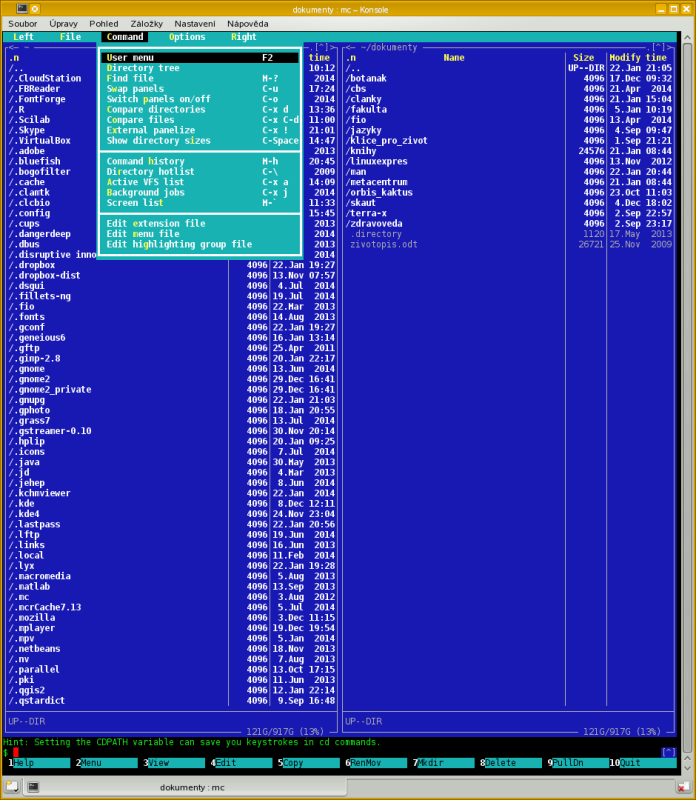
\includegraphics[height=6.5cm]{mc.png}
  \end{multicols}
\end{frame}

\subsection{Archives}

\begin{frame}{Compressing files into archives}
  \begin{center}
    \begin{tabular}{llll}
      \textbf{Archive} & \textbf{Compressing command}\\
      *.tar & tar cvf archive.tar file1 file2\\
      *.tar.gz\alert{/}*.tgz & tar czvf archive.tar.gz\alert{/}.tgz file1 file2\\
      *.tar.bz\alert{/}*.tbz\alert{/}*.tar.bz2 & tar cjvf archive.tar.bz\alert{/}.tbz\alert{/}.tar.bz2 file1 file2\\
      *.tar.xz & tar cvf - file1 file2 | lzma > archive.tar.xz\\
      *.gz & gzip file\\
      *.bz2 & bzip2 file\\
      *.xz & lzma file\\
      *.zip & zip -r archive.zip file1 file2\\
      *.rar & rar a archive.rar file1 file2
    \end{tabular}
  \end{center}
  \begin{itemize}
    \item \texttt{gzip}, \texttt{bzip2} and \texttt{lzma} are able to pack only one file -- use them together with \texttt{tar} to pack multiple files
    \item \texttt{gzip}, \texttt{bzip2} and \texttt{lzma} when used \textbf{without} \texttt{tar} \alert{move} file into archive
    \item \texttt{lzma} has excellent compression, but can be very slow
  \end{itemize}
\end{frame}

\begin{frame}{Compressing and decompressing archives}
  \begin{center}
    \begin{tabular}{llll}
      \textbf{Archive} & \textbf{Decompressing command}\\
      *.tar & tar xvf archive.tar\\
      *.tar.gz\alert{/}*.tgz & tar xzvf archive.tar.gz\alert{/}.tgz\\
      *.tar.bz\alert{/}*.tbz\alert{/}*.tar.bz2 & tar xjvf archive.tar.bz\alert{/}.tbz\alert{/}.tar.bz2\\
      *.tar.xz & lzcat archive.tar.xz | tar xvf -\\
      *.gz & gunzip archive.gz\\
      *.bz2 & bunzip2 archive.bz2\\
      *.xz & unlzma archive.xz\\
      *.zip & unzip archive.zip\\
      *.rar & unrar x archive.rar
    \end{tabular}
    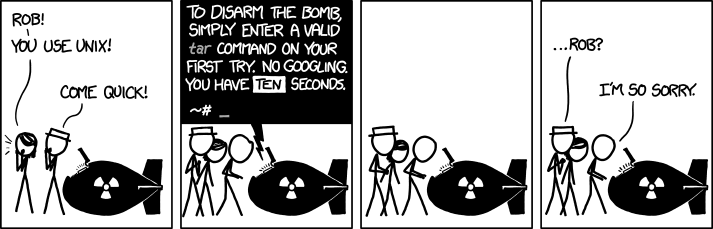
\includegraphics[height=2cm]{tar.png}
    \hfill
    \url{https://xkcd.com/1168/}
  \end{center}
\end{frame}

\subsection{Searching}

\begin{frame}[fragile]{Looking for files and applications}
  \begin{bashcode}
    apropos keyword # Searches for command descriptions containing keyword
    updatedb # Must be regularly launched to get "locate" to work
             # It is usually regularly launched by cron task (see further)
    locate somename # Searches for files/directories in local database
    which # Full path to application (shell command)
    whereis # Path to source code, executable and man pages for the command
    # Test if executable command exists (good for scripts)
    # If "Application" is missing, script ends with error
    command -v Application >/dev/null 2>&1 || { echo >&2 "Application is
      required but not installed. Aborting."; exit 1; }
    command -v find # Behaves like which, but reliable in scripts
    type Application >/dev/null 2>&1 || { echo >&2 "Application is
      required but not installed. Aborting."; exit 1; }
    hash Application 2>/dev/null || { echo >&2 "Application is required
      but not installed. Aborting."; exit 1; }
    exit 1 # Use to be added (with various numbers) after any error to
           # send term signal 1 - for better handling of various errors.
           # Every termination has exit status number - 0 is normal exit.
           # Exit status 1 and higher number is various error.
  \end{bashcode}
\end{frame}

\begin{frame}[fragile]{Find}
  \begin{bashcode}
    find <where> <what> <what to do> # The most powerful searching tool:
    find /.. -type d/f -name XXX -print # Most common usage
  \end{bashcode}
  \begin{itemize}
    \item First \texttt{find}'s parameter is location to search -- absolute or relative, ``\texttt{.}'' means current directory (the only compulsory parameter)
    \item \texttt{-type} for only directories \texttt{d} or only files \texttt{f} (without this parameter, files as well as directories are looked for)
    \item \texttt{-name} of the searched files/directories supports wildcarts (\texttt{*}, \texttt{?} and \texttt{[\ldots]}), see globbing (slide~\ref{globbing})
    \item \texttt{-print} is default action -- prints list of results
    \item \texttt{-exec} runs some command with results (some operation, not just listing)
    \begin{itemize}
      \item All following arguments are argument of the command until ``\texttt{;}'' is encountered
      \item \texttt{\{\}} is replaced by the current file name being processed
      \item Those constructs might require protection by escape (``\textbackslash'') or quotes not to be expanded by shell
    \end{itemize}
  \end{itemize}
\end{frame}

\begin{frame}[fragile]{Find examples}
  \begin{bashcode}
    # Find in photos subdir all JPG files and resize them to 1000x1000 px
    find photos/ -name *.jpg -exec mogrify -resize 1000x1000 '{}' \;
    # Another possibility with xargs (it chains commands - reads input from
    # stdin and execute command with given arguments, using all CPU threads)
    # Note in the example below -print is not needed as it is default action
    find photos/ -name *.jpg | xargs mogrify -resize 1000x1000
    # Find all R scripts in ~/Documents and find in them lines with "DNA"
    find ~/Documents -name *.r -print | grep -nH DNA # Two possibilities
    find ~/Documents -name *.r -exec grep -nH DNA '{}' \;
    # How many directories are there in the books directory
    find books/ -type d -print | wc -l # wc -l calculate lines
    # Find in /home/$USER/photos all JPG files containing string "trip"
    find /home/$USER/photos -name *trip*.jpg -print
    # Change permissions of all files within "files" directory to 777
    find files/ -type f -exec chmod 777 '{}' \;
    # Find all executable files within current directory and list them
    find . -executable -type f -print
    find doc/ -type d -empty -execdir rmdir {} \; # Delete empty directories
    man find # See another options. Much more...
  \end{bashcode}
\end{frame}

\subsection{Network}

\begin{frame}[allowframebreaks]{Network protocols}
  \begin{itemize}
    \item SSH -- secure shell -- command-line connection to remote server to work there (port 22)
    \item Telnet -- old deprecated insecure version of SSH, never ever use it (port 23)
    \item FTP -- file transfer protocol -- outdated, no encryption (port 21)
    \item FTPS -- FTP with added connection encryption for higher security (port 21)
    \item SFTP -- FTP over SSH -- common, secure (port 22)
    \item SCP -- secure copy -- uses SSH, but has restricted possibilities, common, secure (port 22)
    \item NFS -- network file share/server -- very common in UNIX world, commonly used to permanently connect to network server, share directories, etc. (port 20049)
    \item webDAV -- file transfer over web (using WWW server) -- not so common, but good (port 80 or 443 -- same as WWW)
    \begin{itemize}
      \item Accompanied by calDav and cardDav to share calendars and address books over the network
    \end{itemize}
    \item SAMBA -- UNIX connection to Microsoft network shares (port 5445)
    \item web -- ``The Internet'' for most of users (port 80 or encrypted 443)
    \item IMAP (port 143 or 993) and SMTP (port 25 or 465) to connect to e-mail server and send mails
    \item Messaging protocols like XMPP (Jabber and derived services like Google Talk or Facebook Messenger), IRC, ICQ, Skype,~\ldots
    \item And much more\ldots
    \item Port number can be changed in configuration of respective server service
    \item All firewalls on the way must allow communication on given port
  \end{itemize}
\end{frame}

\begin{frame}[fragile]{Basic network information and testing}
  \begin{bashcode}
    hostname # Get name of the computer
    ping web.natur.cuni.cz # Ping host. Is it alive? Cancel by Ctrl+C
    traceroute www.metacentrum.cz # Get route to the host
    mtr hostname # Combines ping and traceroute, quit with "q"
    ip a s # Information about all network devices (MAC, IP address, ...)
    ifconfig -a # Older version of above command
    iwconfig # List of network interfaces
    ip r # Show routes
    nc -vz web.natur.cuni.cz 22 # Does SSH work on the host?
      # verbose (-v), scan (-z), host, port number (22 for SSH, can be any)
    man nc # See for more information; "nc" is alias for "netcat"
    netstat -atn # Information about all network connections
    netstat -ntplu # Show open TCP/UDP ports
    netstat -anp # Show active connections
    netstat -h # See for explanation of 3 above examples
    # If using nmap at faculty, firewall disconnects you for 10 minutes!
    nmap -r someserver.cz # Scan someserver.cz for opened ports
    nmap botany.natur.cuni.cz --script ssh-hostkey # See SSH key
  \end{bashcode}
\end{frame}

\begin{frame}[fragile]{Connecting file systems on remote servers}
  \begin{itemize}
    \item Target mount point must exist before mounting
    \item Servers can be accessed by IP address or hostname
  \end{itemize}
  \begin{bashcode}
    # Mount Windows server (requires package samba)
    mount.cifs //windows.server.cz/Some/Directory /mnt/win -o \
      credentials=/path/to/password.file,uid=USER,gid=GROUP
    # "password.file" contains login credentials to Windows server:
    username=user.name
    password=TopSecretPassword1
    domain=DOMAINNAME
    man mount.cifs # See for other connection options
    # Mounting remote server over SSH (sshfs package must be installed)
    sshfs user@vyuka.natur.cuni.cz:/some/dir /local/mount/point
    # Mount NFS share (NFS is common protocol in UNIX world)
    mount -t nfs some.server.cz:/shared/directory /local/directory
    # Mount webDAV folder (requires package davfs2 to be installed)
    mount -t davfs https://owncloud.cesnet.cz/directory /local/directory
  \end{bashcode}
\end{frame}

\begin{frame}[fragile]{Transferring files from/to remote server}
  \label{transfers}
  \begin{itemize}
    \item \texttt{curlftpfs} allows mount FTP as local directory, but FTP is outdated, insecure and not constructed to that usage\ldots
  \end{itemize}
  \begin{bashcode}
    wget http://some.address.cz/internet # Download file(s) from Internet
    wget --help # -r for recursive download (whole web), -k to convert links
    # curl is predecessor of wget, without parameter "-o" it prints remote
    # content to standard output (typically screen)
    curl http://some.server.cz/some/files -o localfilename
    # Copy files (-r for recursive) over SSH from local computer
    # to remote server or vice versa (just flip arguments)
    scp -r localfiles remoteuser@remote.server.cz:/remote/path/
    scp -r remoteuser@remote.server.cz:/remote/files /local/directory/
    # scp behaves like cp, but works over SSH
  \end{bashcode}
  \begin{itemize}
    \item \texttt{rsync} is synchronization tool (commonly used for backups) able to connect to remote server (next slide)
    \item On server side, same files can be accessible (shared) by more methods
  \end{itemize}
\end{frame}

\begin{frame}[fragile]{Synchronization with rsync}
  \begin{itemize}
    \item \texttt{rsync} has huge amount of possibilities (see \texttt{man rsync} or \texttt{rsync -h})
    \item Works locally as well as over network
    \item It transmits only changes -- very efficient
    \item Suitable for local as well as network backup
    \item Network address for rsync is written in same way as for \texttt{scp}
    \item \texttt{--delete} delete in target location files which are not in source location any more
    \item \texttt{--progress} show progress percentage for every file
    \item \texttt{--exclude=*.jpg} skip JPG files
    \item For incremental backups use \texttt{duplicity}
  \end{itemize}
  \begin{bashcode}
    rsync -arv somedirectory otherplace # All attributes, recursive, verbose
    rsync -arv localdirectory user@remote.server.cz:/remote/directory/
    rsync -arv user@remote.server.cz:/remote/data local/directory/
  \end{bashcode}
\end{frame}

\begin{frame}[fragile]{Connect to SSH with key}{No need to remember password for every server\ldots}
  \begin{bashcode}
    # Create the key
    ssh-keygen -t rsa -b 4096 # Good security, portable
    # ECC gives better security, but not all servers/applications support it
    ssh-keygen -t ecdsa -b 521 # Higher security
    ssh-keygen -t ed25519 # Same security as ecdsa, higher performance
    # Empty (no) passphrase will connect to server without password
    # Copy public key to remote server (private key must be kept locally)
    ssh-copy-id user@remote.server.cz # or
    cat ~/.ssh/XXX.pub | ssh user@remote.server.cz \
      "mkdir -p ~/.ssh && cat >> ~/.ssh/authorized_keys"
    # Now, public key is on the server and private key in local computer is
    # unlocking the connection
    # Unlock the key (no need in some distributions or if there is no
    # passphrase) - must be done only once per user session
    ssh-add
    # Connect as usually
    ssh user@remote.server.cz
  \end{bashcode}
\end{frame}

\begin{frame}{Faculty web server}
  \begin{itemize}
    \item Login requires same credentials as to \href{https://cas.cuni.cz/}{CAS} (login name, no ISIC number)
    \item Faculty information are \href{https://www.natur.cuni.cz/fakulta/cit/web-aplikace/webhosting}{only in Czech}
    \item It is Linux server running Debian
    \item Connect with SSH/SFTP/SCP to \texttt{web.natur.cuni.cz}
    \item Mainly used for webhosting, user's address will have form \texttt{https://web.natur.cuni.cz/$\sim$loginname/}, user can \href{https://helpdesk.natur.cuni.cz/servlet/HelpdeskDynamic?eid=Rozcestnik}{apply} for another URL
    \item Every department also has dedicated space there, it can be used for various web projects, address can be discussed with \href{https://www.natur.cuni.cz/fakulta/cit/lide}{IT department}
    \item Personal web can be placed in \texttt{public\_html} within home folder
    \item Users can \href{https://helpdesk.natur.cuni.cz/servlet/HelpdeskDynamic?eid=Rozcestnik}{apply} for MySQL database or special settings
    \item \href{https://www.natur.cuni.cz/biology/botany/working-information/servers-webs-computers/}{Department of Botany} (and some other departments) have their own web and file servers
  \end{itemize}
\end{frame}

\subsection{Parallelisation}

\begin{frame}{Parallelisation with GNU Parallel}
  \begin{itemize}
    \item \href{https://www.gnu.org/software/parallel/}{GNU Parallel} can distribute task among CPU threads of one computer, or even among different computers in network
    \item It is not effective for short/small tasks
    \item Important operands (for more see \texttt{man parallel})
    \begin{itemize}
      \item \texttt{\{\}} -- input line -- whole line read from input source (typically standard input)
      \item \texttt{\{.\}} -- input line without extension
      \item \texttt{\{/\}} -- base name of input line -- only file name (without path)
      \item \texttt{\{//\}} -- dirname from input line (filename is removed)
      \item \texttt{\{/.\}} -- base name of input line without extension
      \item \texttt{:::} -- use arguments from command line instead of stdin (::: is placed after the command and before the argument)
      \item \texttt{::::} -- read from argument files
      \item \texttt{-j} -- number of jobs -- if not provided, \texttt{parallel} will use all available CPU threads
    \end{itemize}
  \end{itemize}
\end{frame}

\begin{frame}[fragile]{GNU Parallel examples I}
  \begin{bashcode}
    # Convert all images from JPG to PNG
    ls -1 *.jpg | parallel --bar convert '{}' '{.}.png'
    # Resize all images ("\" marks that command continue on next line)
    find . -name '*.jpg' -print | parallel convert -resize 500x500 \
      -quality 75 '{}' '{.}-small.jpg' # or
    parallel convert -resize 25% '{}' '{.}-small.jpg' ::: *.jpg
    # Find WORD in huge text file (named "longfile" here) - this works
    # but it is not possible to get line number (file is red in blocks)
    parallel --pipe --block 10M -- grep --color=always WORD < longfile
    # Same as above but add line numbers according to original file
    nl longfile | parallel -k --pipe --block 20M -- grep WORD
    # When needed to get phrase or regular expression (use parameter
    # "-q" for escaping of shell special characters or extra quotes):
    # "--" stops reading parameters for parallel
    nl longfile | parallel -qk --pipe --block 20M -- grep "WORD TEXT" # or
    nl longfile | parallel -k --pipe --block 20M -- grep '"WORD TEXT"'
    # Convert all WAV files into OGG
    parallel -X oggenc ::: *.wav # -X parse as many parameters as possible
  \end{bashcode}
\end{frame}

\begin{frame}[fragile]{GNU Parallel examples II}
  \begin{bashcode}
    # Run in parallel commands from command list file (list of commands)
    parallel < command_list.txt # (each command on one line) or
    parallel :::: command_list.txt
    # Add same text to the end of multiple files
    ls -1 *.txt | parallel 'cat block_to_be_added.txt >> {}'
    # Replace particular text in multiple files with sed and GNU Parallel
    ls -1 *.txt | parallel 'sed -i "s/XXX/YYY/g" {}'
    # Launch MrBayes for multiple nexus files and create log file with
    # starting and ending date and time
    ls -1 *.nexus | parallel 'echo -e "Start: `date`\n" > {}.log && mb {} |
      tee -a {}.log && echo "End: `date`" >> {}.log'
    # tee (-a for append to existing file) records output of MrBayes
    command | tee record.txt # tee will record whole output of command
    tee record.txt | command # tee will record user input
    # If software reads commands from user, we can reuse record next time:
    command < record.txt # Empty lines are interpreted as Enter key
                         # Each line is used whenever command waits for new
                         # input (instead of typing, record.txt is used)
  \end{bashcode}
\end{frame}

\subsection{Timing}

\begin{frame}[fragile]{Launching of tasks at certain time}
  \begin{itemize}
    \item \texttt{at} can run command at certain time (atd daemon must be running)
    \item Tasks are running in background, outputs are mailed (e.g. to \texttt{/var/spool/mail/\$USER})
  \end{itemize}
  \begin{bashcode}
    # Check status of atd daemon (it must run), start/stop/enable/disable it
    systemctl status/start/stop/enable/disable atd.service
    man at # Check for various possibilities of time settings
    at HH:MM # Run commands at certain time (hour:minutes)
    at> command1 # Add as many commands as you wish (separate by Enter)
    at> # When done, press Ctrl+D to cancel giving commands to at
    # Instead of manual typing of tasks, run script at certain time
    at HH:MM -f somescript.sh # Run somescript.sh at certain time
    at -l # List of scheduled tasks (alias is atq)
    at -r <number> # Cancel scheduled task (according to number from at -l)
    atrm # Alias for previous command
    batch # Commands will be executed when system loads drops below 0.8 or
          # other value specified in configuration or startup of atd
  \end{bashcode}
\end{frame}

\begin{frame}[fragile]{Automated launching of tasks}
  \begin{itemize}
    \item \texttt{cron} runs tasks repeatedly (cron daemon must be running)
    \item Scripts for tasks running hourly/daily/weekly/monthly can be copied into respective \texttt{/etc/cron.*/} directories
  \end{itemize}
  \begin{bashcode}
    # Check status of cron daemon (it must run), start/stop/enable/disable
    systemctl status/start/stop/enable/disable cron.service
    crontab -l # List user's cron tasks
    crontab -e # Edit user's cron tasks:
    # Minute, Hour, Day in month, Month, Day in week, Command (absolute path)
    # 0-59    0-23  1-31          1-12   0-6 starting with Sunday (WTF?)
      *       *     *             *      *            /usr/bin/command
      10      22    1             *      *        # 1st day in month, 23:11
      0       */3   *             *      *        # Every 3 hours
      0       11    *             *      0        # Every Sunday, 12:00
      30      3     */2           *      *        # Every even day, 4:31
      */15    *     *             *      0,4   # At Sun and Fri every 15 min
    # Columns are separated by any number of spaces
  \end{bashcode}
\end{frame}

\section{Text}

\begin{frame}{Everything is (text) file}
  \begin{itemize}
    \item As UNIX configuration and outputs (logs,~\ldots) are mostly saved as relatively simple text files, manipulations of any type with text files is one of the most common tasks
    \begin{itemize}
      \item Similar situation is for molecular data -- input/output data use to be text files with simple structure
    \end{itemize}
    \item One of the most powerful features of BASH
    \item Some operations are complicated (e.g. complex manipulations with columns, various calculations) it is necessary to use AWK or Perl (probably the most advanced language working with text)
    \item Text-manipulating tools have very rich implementation of regular expressions (slide~\ref{regexp})
    \item Most of the operations are done in stream -- per line -- everything is very fast
  \end{itemize}
\end{frame}

\subsection{Reading}

\begin{frame}[fragile]{Read text file}
  \begin{bashcode}
    cat # Read or join files (-n adds line numbers, -v prints non-printable
        # characters like EOL)
    cat textfile # Print content of text file
    cat textfile1 >> textfile2 # Append textfile1 to the end of textfile2
    nl textfile # Like cat -n, prints textfile with line numbers
    tac textfile # Like cat, but prints lines in reverse order
    more textfile # When textfile is long, prints screen by screen (space
                  # for next screen, q to quit)
    less textfile # Better version of more - you can scroll up and down by
                  # PgUp, PgDown, arrows, searching by / (type searched
                  # string, hit Enter, n for next, twice ESC to quit),
                  # q to quit viewing (also used by man)
    most textfile # Better version of less
    fmt textfile # Basic formatting of text - joining of commented lines,
                 # line breaks to break too long lines, ...
    fmt textfile > formatted_file # Save output of fmt into new file
    wc textfile # lines, words and bytes in text file
                # wc -l for only lines, -m for characters, -w for words
  \end{bashcode}
\end{frame}

\subsection{Extractions}

\begin{frame}[fragile]{Get part of text file (by lines)}
  \begin{bashcode}
    head -n N textfile # Print first N lines from textfile
    tail -n N textfile # Print last N lines from textfile
    head -n-N textfile # Print textfile without last N lines
    tail -n+N textfile # Print textfile from Nth line to the end
    # Split text file on selected pattern - creates new files xxXY
    csplit textfile '/pattern/' '{*}' # pattern itself is inside '/___/'
    # Pattern can be regular expression - set it carefully
    # {*} says to repeat operation as many times as possible
    grep -parameters pattern textfile # Write lines containing pattern
    grep user /etc/passwd # Write all lines in passwd containing user
    cat /etc/passwd | grep user # Same as above
    grep -v user /etc/passwd # Write all lines in passwd NOT containing user
    grep -c user /etc/passwd # Get number of lines in passwd containing user
    grep -i USER /etc/passwd # -i isn't case sensitive
    grep -q ... # quiet - no output - good for testing in scripts
    grep -ls user /etc/* # -l print files with pattern, -s suppresse errors
    grep "longer text" textfile # Extract whole phrase
  \end{bashcode}
  \begin{itemize}
    \item Grep supports regular expressions, slide \ref{regexp}
  \end{itemize}
\end{frame}

\begin{frame}[fragile]{Work with columns}
  \label{cutpaste}
  \begin{itemize}
    \item \texttt{cut} extracts columns, \texttt{paste} joins, \texttt{column} reformates
    \item BASH can not select column according to its name (Perl can do that)
  \end{itemize}
  \begin{bashcode}
    cut column/delimiter+field textfile
    cut -c 1 /etc/group # Get first character
    cut -c 1-5 /etc/group # Get character 1-5
    cut -c 4- /etc/group # Get character 4 and more
    cut -c 2,5,7 /etc/group # Get characters 2, 5 and 7
    cut -d ':' -f 1 /etc/group # Select 1st field separated by ":"
    cut -d ':' -f 2-4 /etc/group # Select fields 2-4 separated by ":"
    cut -f 1,2 cut_awk_test_file.tsv # get columns 1 and 2 separated by TABs
    # Add second file as second column
    paste file1 file2 > outputfile
    # Output will be two columns (from file1 and file2) separated by TAB
    paste -d "|" diff_test_file_1.txt diff_test_file_2.txt # -d for delimiter
    # Swapping columns is not very comfortable...
    paste <(cut -f2 cut_awk_test_file.tsv) <(cut -f1 cut_awk_test_file.tsv)
    ls -l | column -t # Reformate input as table (compare with ls -l)
  \end{bashcode}
  \vfill
\end{frame}

\subsection{AWK}

\begin{frame}[fragile]{Get a column with awk}
  \begin{itemize}
    \item AWK is scripting language mainly for text manipulations
    \item Can not select column according to its name (Perl can do that)
    \item Can do things other BASH tools can not do (easily) -- better manipulation with columns, calculations,~\ldots
    \item Has complicated syntax, it is hard to read, it is not similar to other tools -- Perl can do more and is more common (learn it instead)\ldots
    \item Supports regular expressions, slide \ref{regexp}
  \end{itemize}
  \begin{bashcode}
    awk 'regexp { commands parameters }' file
    awk '{print $NF}' textfile # Select last column (separated by tab)
    awk '{print $2}' textfile # Select 2nd column (separated by tab)
    awk '{print $3, $2}' textfile # Print columns 3 and 2 (in this order)
    awk -F ' ' '{print $4, $1}' textfile # Print columns 4 and 1
                                         # separated by " " (space)
    ls -l | awk '/^d/ { print $8 "\t" $3 }' # Separate columns by TAB
               # /^d/ for lines starting with "d" (only directories)
  \end{bashcode}
  \vfill
\end{frame}

\begin{frame}[fragile]{More AWK examples}
  \begin{bashcode}
    # Print on even lines ">", former column 1, new line, former column 2
    awk '{print ">"$1"\n"$2}' awk_test_file.tab # 2 columns into 2 lines
    # Print field 1, TAB (\t), length of field 2, TAB and field 2
    awk '{print $1"\t"length($2)"\t"$2}' textfile
    # If field 1=1, print whole line
    awk '{if($1==1){print $0}}' textfile
    # Field 1 is numeric (less then 5 digits) - add leading zeroes
    awk '{printf "%05d\n", $1;}' textfile
    # As above, but add leading zeroes to field 1 and print whole line
    awk '{$1=sprintf("%05d", $1); print $0}' textfile
    # Field 6 is numeric, select lines where field 6 is higher than 100
    awk -F '\t' '$6>100' cut_awk_test_file.tsv # Separated by TABs (\t)
    # Print fields 4 and 5 (fields are separated by "_" or TAB)
    awk -F '[_\t]' '{print $4, $5}' awk_test_file.tab
    # Precede each line by its line number for all files together, with TAB
    awk '{print NR "\t" $0}' diff_test_file_*
    # substitute "foo" with "bar" ONLY for lines which contain "baz"
    awk '/baz/{gsub(/foo/, "bar")}; 1'
  \end{bashcode}
\end{frame}

\subsection{Manipulations}

\begin{frame}[fragile]{Sorting}
  \begin{bashcode}
    sort textfile # Sort a text file
    sort -d textfile # Take into account only spaces and alphanumerical
                     # characters (ignore any other characters)
    sort -r textfile # Reverse order
    sort -f textfile # Ignore character case (not case sensitive)
    sort -m textfile1 textfile2 # Merge already sorted text files
    sort -u textfile # Print only first of multiple entries
    sort -b textfile # Ignore leading blanks (space on beginning of line)
    # Sorting is influenced by locale setting (e.g. Czech "ch")
    LC_ALL=C sort ... # To force use of English locale use
    sort -k 2 -n textfile # Sort according to 2nd field (numerically)
    uniq textfile # Filters following identical lines - only unique
                  # are printed (to get unique lines from whole file,
                  # sort it first)
    uniq -c textfile # Add number of occurrences before each line
    uniq -d textfile # Print only repeated lines
    uniq -i textfile # Ignore case (not case sensitive)
    uniq -s N textfile # Skip first N characters
    uniq -u textfile # Print only not-repeated lines
  \end{bashcode}
\end{frame}

\begin{frame}[fragile]{Replacements -- tr}
  \begin{itemize}
    \item \texttt{tr} replaces or deletes characters from standard input and writes result to standard output -- use pipes and/or redirects
  \end{itemize}
  \begin{bashcode}
    # Replace space by TAB in inputtextfile, save result as outputtextfile
    cat inputtextfile | tr " " "\t" > outputtextfile
    # Delete "text" from each line and print it to standard output (screen)
    cat inputtextfile | tr -d "text"
    # Replace every occurrence of A, B, C or D by a new line (\n)
    cat inputtextfile | tr "[ABCD]" "\n" > outputtextfile
    # Replace capital letters by small ones
    tr "[A-Z]" "[a-z]" < inputtextfile > outputtextfile
    # Alternative (easier reading) of previous command:
    cat inputtextfile | tr "[:upper:]" "[:lower:]" > outputtextfile
    # Replace all new lines (line breaks) by TABs
    cat inputtextfile | tr "\n" "\t"  > outputtextfile
    # Discard all new lines - output will be one line
    tr -d "\n" < textfile > /dev/stdout # stdout is typically screen
    tr --help # See another possibilities for pattern to find/replace
  \end{bashcode}
\end{frame}

\begin{frame}[fragile]{Replacements with sed}
  \begin{itemize}
    \item \texttt{sed} supports regular expressions, see slide \ref{regexp} (same as in \texttt{grep} and \texttt{vim}), with parameter \texttt{-r} can use extended regular expressions (do not confuse -- the syntax is slightly different, richer)
    \item Output is written to standard output -- use pipes, redirects or \texttt{-i} to modify the file in place (without printing of output)
    \item Mac OS~X has old outdated versions of \texttt{grep}, \texttt{sed} and other tools (richness of regular expressions is poor) -- use versions from \href{http://brew.sh/}{Homebrew} or search documentation how to modify the patterns\ldots
    \item Option \texttt{-s} separates multiple files (otherwise lines in multiple files are calculated as one stream)
    \item Option \texttt{-n} use to be used when deleting lines or printing only specific lines to suppress other lines (see examples)
    \item Various parameters, modificators, operators can be combined\ldots
  \end{itemize}
  \begin{bashcode}
    sed 'operator/FindToReplace/Replace/modificator' textfile > newtextfile
  \end{bashcode}
  \vfill
\end{frame}

\begin{frame}[fragile]{Sed examples I}
  \label{sedex}
  \begin{bashcode}
    # Search and replace ("s") all occurrences ("g") of "find" by "replace"
    sed 's/find/replace/g' textfile
    # Replace third occurrence of pattern on every line
    sed 's/pattern/Replace/3' # 's/.../.../' replace only first occurrence
    sed '1,7s/...' # To work only on particular line, place single number or
    sed '5s/...'   # range (e.g. 1,7) right before "s" ("$" for last line)
    sed '1~2n;s/F/R/g' # Work on every second line, starting by line 1
    sed -n '2~10p' # Print every 10th line, starting with line 2
    seq 1 100 | sed -n '2~10p' # Example of above pattern (see "seq 1 100")
    # Replace first TAB (\t) on each line by new line (\n)
    sed 's/\t/\n/' textfile
    sed 's/find/replace/g' somedirectory/* # Work on all files in directory
    # Convert all capital letters into lower
    sed 's/[A-Z]/\L&/g' inputtextfile > outputtextfile # And vice versa:
    sed 's/[a-z]/\U&/g' inputtextfile > outputtextfile
    # Groups to remember work in same way in sed, grep as well as vim
    \(ToRemember\) # Remember expression in brackets (example at next slide)
    \Number # Use remembered expression (numbered from one: \1, \2, \3, ...)
  \end{bashcode}
\end{frame}

\begin{frame}[fragile]{Sed examples II}
  \begin{bashcode}
    # Take output of ls -l and replace value of $USER by "$USER-RULEZZZ"
    ls -l | sed "s/\($USER\)/\1-RULEZZZ/g" # Note " to use variable
    # Replace size column (2nd numeric) by "size:TAB<file size>b"
    # Second sed replaces any white spaces by single TAB
    ls -l | sed 's/\([0-9]\+\)/size:\t\1b/2' | sed 's/[[:blank:]]\+/\t/g'
    sed '/^$/d' # Delete blank lines ('8d' line 8, 's/ *$//' spaces on EOL)
    sed '/GUI/d' # Delete all lines containing "GUI" ('s/GUI//g' only "GUI")
    sed '5 i\Linux is great.' # Insert to 5th line ('4 a\' after 4th line)
    # Insert text to the beginning of the 3rd line (compare with previous)
    sed '3s/^/INSERT/' # ^ is beginning of line, $ end ('$/...' last line)
    # From ls -l keep number of links (1st numeric column after permissions)
    # and then flip user and group and print it as "group:user"
    ls -l | sed 's/ \([[:digit:]]\+\) \([[:alnum:]]\+\) \([[:alnum:]]\+\) /
      \1 \3:\2 /g' # Note separating spaces (previous line ends with space)
    # Escaping - replace dot by comma (dot means any single character)
    sed 's/\./,/g' # \ escapes following character (compare with 's/./,/g')
    # Replace any of characters within [...] by some pattern
    sed 's/[abcd]/X/g' # Compare with reverse case 's/[^abcd]/X/g'
  \end{bashcode}
\end{frame}

\begin{frame}[fragile]{Joining}
  \begin{itemize}
    \item Generally, most of tools work per-line, \texttt{paste} appends columns (slide~\ref{cutpaste})
    \item Join compares every matching lines (by default 1$^{st}$ field) and creates all combinations - ensure to have sorted input files with unique text
    \begin{itemize}
      \item E.g. if 1$^{st}$ file contains \texttt{A B} and \texttt{A C} and 2$^{nd}$ file \texttt{A D} and \texttt{A E}, the result will be \texttt{A B D}, \texttt{A B E}, \texttt{A C D} and \texttt{A C E}
    \end{itemize}
  \end{itemize}
  \begin{bashcode}
    # Add file to the end of another text file
    cat file1 >> file2 # file2 will contain both files, file1 is unchanged
    # Compare two sorted text files and write shared lines
    # (duplicitous lines are shown just once)
    join textfile1 textfile2 > outputfile
    # If used on wrong files, it can create huge file
    seq -f "1 %g" 100 > aaa && less aaa
    seq -f "1 %g" 100 > bbb && less bbb
    join aaa bbb | wc -l
    join --help # See more options...
  \end{bashcode}
  \vfill
\end{frame}

\subsection{Comparisons}

\begin{frame}[fragile]{Comparisons}
  \begin{bashcode}
    cat diff_test_file_1.txt diff_test_file_2.txt # See and use examples
    # Compare two sorted columns
    comm textfile1 textfile2
      # 1st column - lines only in textfile1
      # 2nd column - lines only in textfile2
      # 3rd column - lines in both files
    comm -2 textfile1 textfile2 # Don't show 2nd column (similarly -1, -3)
    # Show differences between text files
    diff textfile1 textfile2
      # First number shows line(s) in 1st file, then if add/delete/change
      # and last number shows line(s) in the second file, <> show direction
    diff -e textfile1 textfile2 # More simple output
    diff -c textfile1 textfile2 # Show context (lines around change)
    diff -u textfile1 textfile2 # Better version, the most common
    diff -y textfile1 textfile2 # In two columns comparing both files
    colordiff # Same usage and parameters as previous, colored output
    diff -u textfile1 textfile2 | view - # Launches vim (exit by :q! Enter)
    vimdiff # Can show more colors, launches vim (exit by :q! Enter)
  \end{bashcode}
\end{frame}

\subsection{Editors} 

\begin{frame}[fragile]{Command line text editors}
  \begin{itemize}
    \item \texttt{nano}, \texttt{pico} and \texttt{mc} are very simple, just for very basic text editing in command line or until you learn \texttt{vim} (graphical version is \textbf{gVim}) or \texttt{emacs} (graphical version is also available, just search for \textbf{Emacs} in your distribution software manager)
    \item You can work most of the time in graphical editors (slide \ref{editors})
    \item Emacs and Vim are extremely rich, but having completely different approach -- when you get use to one, you can't use the another
  \end{itemize}
  \begin{bashcode}
    nano textfile # Enhanced clone of pico, basic simple text editor
    pico textfile # Basic simple text editor
    mc # Use its internal editor, just very basic (press F4 on the file)
    emacs textfile # Extremely feature rich (including file browser
                   # and many tools), Exit by Ctrl+X and Ctrl+C
    vim textfile # Probably the most common, as rich as Emacs (see further)
    vimtutor # Launch tutorial to learn Vim (in various languages)
   \end{bashcode}
\end{frame}

\begin{frame}{The editors and their usage}
  \begin{itemize}
    \item In \texttt{nano} and \texttt{pico} see bottom line for commands
    \begin{itemize}
      \item \texttt{Ctrl+O} to write the file, \texttt{Ctrl+X} to quit the editor, \texttt{Ctrl+G} for help (\texttt{\textasciicircum}~stands for \texttt{Ctrl} key)
    \end{itemize}
    \item In \texttt{mc} highlight the file to edit and press \texttt{F4}
    \begin{itemize}
      \item \texttt{F2} to save, \texttt{F10} to quit, \texttt{F1} to help, \texttt{F9} for top menu (navigate with arrows, cancel with double \texttt{Esc}), it is possible to use mouse
    \end{itemize}
    \item \textbf{Emacs} use huge number of commands with \texttt{Ctrl} key
    \begin{itemize}
      \item See \url{https://www.gnu.org/software/emacs/tour/}, \url{http://tuhdo.github.io/emacs-tutor.html} and \url{http://www.jesshamrick.com/2012/09/10/absolute-beginners-guide-to-emacs/}
    \end{itemize}
    \item The most common is \textbf{Vim} (next slide)
    \begin{itemize}
      \item See \url{http://vim-adventures.com/} to play a game and learn Vim
    \end{itemize}
    \item \textbf{Emacs} and \textbf{Vim} have huge number of possibilities and support for plugins and scripts, but completely different usage style -- one person can really learn only one\ldots
  \end{itemize}
\end{frame}

\begin{frame}{Vim}{Vim has three different working modes}
  \begin{enumerate}
    \item \textbf{``Normal''} -- nothing is displayed in bottom left corner, every key has some meaning (\texttt{dd} to cut current line, \texttt{r} to replace character below cursor, \texttt{v} for selection of text, \texttt{y} to copy, \texttt{x} to cut, \texttt{p} to paste, \texttt{i} or \texttt{Insert} key to enter insert mode, \texttt{:} to enter command mode, number to get to line of particular line number, \texttt{u} to undo last change(s),~\ldots)
    \item \textbf{Insert} -- in bottom left corner ``\texttt{-- INSERT --}'' is displayed -- the most familiar mode -- normal typing etc., exit to normal mode by \texttt{ESC} key
    \item \textbf{Command} -- in bottom left corner \texttt{:} is displayed -- awaits commands, e.g. \texttt{w} to write file, \texttt{q} to quit, \texttt{q!} to quit and discard changes, \texttt{\%s/\ldots} to search and replace as in \texttt{sed}, \texttt{syntax on/off} to turn syntax highlight on/off, \texttt{/ToSearch} to search (\texttt{Enter}, \texttt{n} for next occurrence, quit with \texttt{Esc}),~\ldots{ }Exit to command mode by \texttt{Backspace} key (delete ``\texttt{:}'').
  \end{enumerate}
  \begin{itemize}
    \item See \url{http://vim.wikia.com/}, \url{http://www.vim.org/docs.php}; česky \url{http://www.nti.tul.cz/~satrapa/docs/vim/}
  \end{itemize}
\end{frame}

\subsection{Regular expressions}

\begin{frame}{Regular expressions are useful\ldots}
  \begin{multicols}{2}
    \begin{center}
      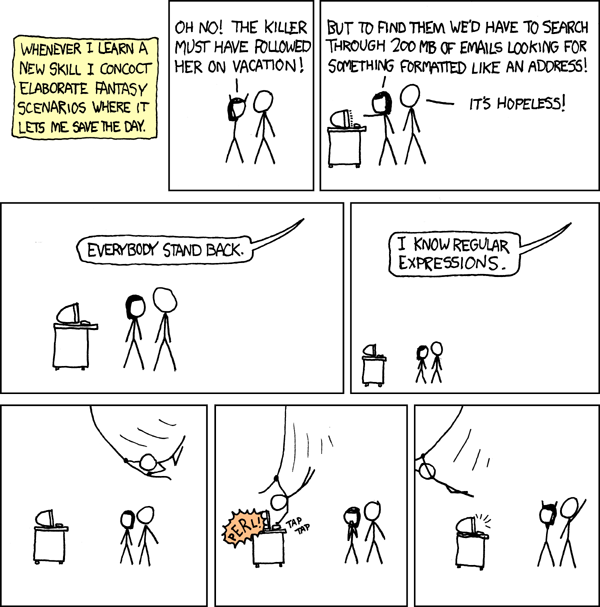
\includegraphics[height=5.5cm]{regular_expressions.png}
    \end{center}
    \columnbreak
    \begin{itemize}
      \item Find text according to a~pattern
      \item Manipulate the text -- flip, reformat, replace,~\ldots
      \item Syntax is variable among programming languages and applications
      \item There are commonly more solutions for one task
      \item Probably the most advanced is Perl
    \end{itemize}
    \vfill
    \url{https://xkcd.com/208/}
  \end{multicols}
\end{frame}

\begin{frame}[allowframebreaks]{Regular expressions}
  \label{regexp}
  \begin{itemize}
    \item \alert{\texttt{.}} -- any single character
    \item \alert{\texttt{*}} -- any number of characters/occurrences of pattern (including 0)
    \item \alert{\texttt{+}} -- one or more occurrences of the preceding reg exp
    \item \alert{\texttt{?}} -- zero or one occurrences of the preceding reg exp
    \item \alert{\texttt{[\ldots]}} -- any character in the brackets
    \item \alert{\texttt{[\textasciicircum\ldots]}} -- reverse case -- all characters except newline and those listed in brackets
    \item \alert{\texttt{\textasciicircum}} -- first character of reg exp -- beginning of the line
    \item \alert{\texttt{\$}} -- last character of reg exp -- end of the line
    \item \alert{\texttt{\textbackslash\{n,m\textbackslash\}}} -- range of occurrences of single character
    \item \alert{\texttt{\textbackslash\{n\textbackslash\}}} -- exactly \textit{n} occurrences
    \item \alert{\texttt{\textbackslash\{n,\textbackslash\}}} -- at least \textit{n} occurrences
    \item \alert{\texttt{\textbackslash}} -- escape following special character
    \item \alert{\texttt{|}} -- either the preceding or following reg exp can be matched (alternation)
    \item \alert{\texttt{\textbackslash(\ldots\textbackslash)}} -- group reg exp (numbered, starting with 1) -- can be called by \alert{\textbackslash\textit{n}}, where \textit{n} is number of the group (starting with 1)
    \item \alert{\texttt{\textbackslash$<$}}, \alert{\texttt{\textbackslash$>$}} -- word boundaries
    \item \alert{\texttt{[[:alnum:]]}} -- alphanumerical characters (includes white space), same like \alert{\texttt{[a-zA-Z0-9]}}
    \item \alert{\texttt{[[:alpha:]]}} -- alphabetic characters, like \alert{\texttt{[a-zA-Z]}}
    \item \alert{\texttt{[[:blank:]]}} -- space and TAB
    \item \alert{\texttt{[[:cntrl:]]}} -- control characters
    \item \alert{\texttt{[[:digit:]]}} -- numeric characters, like \alert{\texttt{[0-9]}}
    \item \alert{\texttt{[[:graph:]]}} -- printable and visible (non-space) characters
    \item \alert{\texttt{[[:lower:]]}} -- lowercase characters, like \alert{\texttt{[a-z]}}
    \item \alert{\texttt{[[:print:]]}} -- printable characters (includes white space)
    \item \alert{\texttt{[[:punct:]]}} -- punctuation characters
    \item \alert{\texttt{[[:space:]]}} -- white space characters
    \item \alert{\texttt{[[:upper:]]}} -- uppercase characters, like \alert{\texttt{[A-Z]}}
    \item \alert{\texttt{[[:xdigit:]]}} -- hexadecimal digits
    \item \alert{\texttt{\textasciicircum\$}} -- blank line
    \item \alert{\texttt{\textasciicircum.*\$}} -- entire line whatever it is
    \item \alert{\texttt{ *}} -- one or more spaces (there is space before asterisk)
    \item \alert{\texttt{\&}} -- content of pattern that was matched
    \item Implementation in \texttt{vim}, \texttt{sed}, \texttt{grep}, \texttt{awk} and \texttt{perl} and among various UNIX systems is almost same, but not identical\ldots
    \item \textbf{grep}, \textbf{sed} and \textbf{vim} \alert{require escaping} of \alert{\texttt{+}}, \alert{\texttt{?}}, \alert{\texttt{\{}}, \alert{\texttt{\}}}, \alert{\texttt{(}} and \alert{\texttt{)}} by backslash \alert{\texttt{\textbackslash}} -- \textbf{egrep} (extended version, launched as \texttt{grep -E \ldots} or \texttt{egrep \ldots}), \textbf{sed} with extended reg exp (\texttt{sed -r}) and \textbf{perl} \alert{not}
    \item Read \url{http://www.regular-expressions.info/}; česky \url{http://www.nti.tul.cz/~satrapa/docs/regvyr/}, \url{http://www.root.cz/serialy/regularni-vyrazy/} and \url{http://www.regularnivyrazy.info/}, and manuals for Grep, Vim, Sed, Awk, Perl,~\ldots
    \item See sed examples, slide~\ref{sedex}
    \item Mac OS~X has by default very outdated version of \texttt{sed} and another tools -- it does not have all advanced features -- users need to install e.g. \texttt{gnu-sed} formulae from \href{http://brew.sh/}{Homebrew}
  \end{itemize}
\end{frame}

\section{Scripting}

\subsection{Basic skeleton}

\begin{frame}[fragile]{Basic script}
  \begin{itemize}
    \item Every script begins with \texttt{\#!/bin/bash} (or alternative for another shells, Perl,~\ldots)
    \item Add any commands you like\ldots
    \item Every script should end with \texttt{exit} (but it is not necessary)
    \item After writing the script, add execution permission (\texttt{chmod +x noninteractive.sh})
    \item Launch with \texttt{./noninteractive.sh}
    \item The most simple script:
  \end{itemize}
  \begin{bashcode}
    #!/bin/bash
    # Simple non-interactive script - no communication with user
    # only list of commands
    echo "Hi, $USER, today is `date` and your PATH is $PATH."
    echo
    exit
  \end{bashcode}
\end{frame}

\subsection{BASH variables}

\begin{frame}{Special variables available in the script (selection)}
  \begin{itemize}
    \item \alert{\texttt{\$1}},~\ldots~(number from \texttt{1} up to number of parameters) -- individual positional parameters (see next slide for example)
    \item \alert{\texttt{\$0}} -- path of the starting script
    \item \alert{\texttt{\$\#}} -- number of command-line arguments
    \item \alert{\texttt{\$*}} -- all of the positional parameters, seen as a single word, must be quoted
    \item \alert{\texttt{\$@}} -- same as \texttt{\$*}, but each parameter is a quoted string -- the parameters are passed on intact, without interpretation or expansion, each parameter in the argument list is seen as a separate word, should be quoted (i.e. something like \texttt{"\$@"})
    \item \alert{\texttt{\$\$}} -- process ID (PID) of the script itself
    \item \alert{\texttt{\$?}} -- Exit status of a command, function, or the script itself
    \item \href{http://www.tldp.org/LDP/abs/html/internalvariables.html}{See more variables\ldots}
  \end{itemize}
\end{frame}

\subsection{Functions}

\begin{frame}[fragile]{Functions in BASH}{Pieces of code, which can be used repeatedly}
  \begin{bashcode}
    # Declare new function
    function MyNewFunction1 {
      echo "Hello, $USER on $HOSTNAME!"
      }
    # Use it in a script as any other command
    ...
    MyNewFunction1
    ...
    # Use with variables - provide parameters for the function
    # See following script examples for another input - same as in scripts
    function MyNewFunction2 {
      echo "The sum is `expr $1 + $2`."
      }
    # Use it in the script
    ...
    MyNewFunction2 5 8 # For example
    ...
  \end{bashcode}
\end{frame}

\subsection{Reading variables}

\begin{frame}{It is important to check user input\ldots}
  \begin{center}
    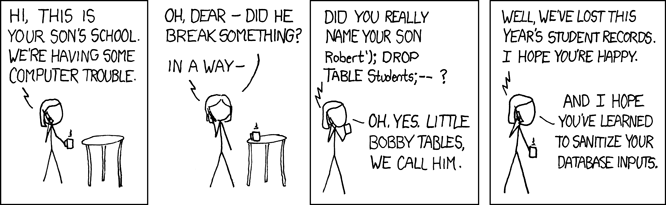
\includegraphics[width=7.5cm]{exploits_of_a_mom.png}
  \end{center}
  \begin{flushright}
    \url{https://xkcd.com/327/}
  \end{flushright}
  \begin{itemize}
    \item By accident or purpose (attack), user can enter unexpected value
    \begin{itemize}
      \item In the ``best'' case, the script ``just'' crashes
      \item Script can behave unexpectedly, returning very weird results
      \item Internal functions/commands can return error messages, which are hard to understand
      \item Attacker can e.g. modify web content (\href{https://en.wikipedia.org/wiki/Cross-site_scripting}{XSS},~\ldots), obtain private data, root privileges,~\ldots
    \end{itemize}
    \item Programmer should always check if user input is correct, filter it
  \end{itemize}
\end{frame}

\begin{frame}[fragile]{Script reading two variables}
  \begin{bashcode}
    #!/bin/bash
    # Arguments are read from command line as parameters of the script
    # Order has to be kept (well, not in this case, but generally yes)
    echo "Sum of two numbers $1 and $2 is `expr $1 + $2`."
    # "$#" is available every time and contains number of parameters
    # (variables) given to the script
    echo "Number of parameters is $#."
    # "$*" is available every time and contains all supplied parameters
    echo "Those parameters were supplied: $*."
    # "$0" is available every time and contains script path
    echo "Path to the scrip is: \"$0\"."
    echo
    exit
  \end{bashcode}
  \vfill
  When done, do:
  \vfill
  \begin{bashcode}
    chmod +x interactive1.sh
    ./interactive1.sh 8 9 # Or select any other two numbers
  \end{bashcode}
  \vfill
  \begin{itemize}
    \item There is no checking of input values, nothing advanced,~\ldots
  \end{itemize}
  \vfill
\end{frame}

\begin{frame}[fragile]{Variables will be interactively provided by the user}
  \begin{bashcode}
    #!/bin/bash
    # Arguments are read from user input (script asks for them)
    echo "Please, input first value to sum and press Enter"
    read V1
    echo "Please, input second value to sum and press Enter"
    read V2
    echo "Sum of two numbers $V1 and $V2 is `expr $V1 + $V2` ."
    echo
    exit
  \end{bashcode}
  \vfill
  When done, do:
  \vfill
  \begin{bashcode}
    chmod +x interactive2.sh
    ./interactive2.sh # Values will be provided when script asks
  \end{bashcode}
  \begin{itemize}
    \item There is no checking of input values, nothing advanced,~\ldots
    \item See next slide to read the variable in \texttt{while} cycles to ensure it is correctly entered
  \end{itemize}
  \begin{bashcode}
    $(expr $1 + $2) # Alternative - $(...) is same as `...`
  \end{bashcode}
\end{frame}

\begin{frame}[fragile]{Ensuring user interactively provides correct input}
  \begin{itemize}
    \item Detailed explanations of all features used here are in various following slides\ldots{ }See scripts \texttt{interactive2\{whiles,functions\}.sh}
  \end{itemize}
  \begin{bashcode}
    ... # Following code replace lines 3 and 4 from previous script
    NUMBER='^[0-9]+$'
    echo "Please, provide a number as input value:"
    while : # Start of while cycles - run until correct input is provided
      do # Star of the body of the cycles
      read INPUT # Here the input from keyboard is received
      if [[ $INPUT =~ $NUMBER ]]; then # Test if INPUT is a number
        echo "OK, input value is $INPUT."
        break # We have correct value, we can break the cyclus and continue
        else # What to do if the user did not provided correct value
          echo "Error! You provided wrong value!" # Tell the user
          echo "Try again (the number):" # Ask user for new input value
        fi # End of the conditional evaluation
      done # End of the while cycles
    ... # The code continues...
  \end{bashcode}
\end{frame}

\begin{frame}[fragile]{Provide named parameters}
  \begin{bashcode}
    #!/bin/bash
    # Script has only one parameter ($1) provided as its parameter
    case "$1" in # evaluating provided parameter and behaving accordingly
      -d|--disk) # "|" means alternatives - more possible inputs
        echo "Your disk usage is:"
        df -h
        ;;
      -u|--uptime)
        echo "Your computer is running:"
        uptime
        ;;
      # This should be every time last possibility - any other input
      *) # User is then notified he entered nonsense and gets some help
        echo "Wrong option!"
        echo "Usage: -d or --disk for available disk space or"
        echo "-u or --uptime for computer uptime"
        exit 1;; # In this case, exit with error code 1
    esac
    exit
  \end{bashcode}
\end{frame}

\begin{frame}{Notes to previous script}
  \begin{itemize}
    \item First make \texttt{interactive3.sh} executable and launch it via e.g. \texttt{./interactive3.sh -d} or \texttt{./interactive3.sh --uptime} or so
    \item Function \texttt{case} has basic checking of input available -- as last parameter use \texttt{*)} -- any other input except those defined above will produce some warning message, error or so
    \item In same way can be added more parameters (by multiple use of \texttt{case}), but order of parameters must be kept and all parameters are compulsory
    \item \texttt{case} can evaluate simple regular expressions, e.g. \texttt{--[Uu]ptime)}, \texttt{-d*},~\ldots
    \item This is the most simple usage, more complex possibilities are ahead
  \end{itemize}
\end{frame}

\begin{frame}[fragile]{Provide parameters, verify them and behave accordingly I}
  \begin{bashcode}
    #!/bin/bash
    NUMBER='^[0-9]+$' # From beginning (^) to the end ($) only number(s) (+)
    function usagehelp { # Function to print help
      echo "Usage: number1 plus/minus/product/quotient number2"
      echo "Use plus for sum, minus for difference, product"
      echo "for multiplication or quotient for quotient."
      exit 1 # End up with an error
      }
    if [ "$#" -ne "3" ]; then # Do we have 3 parameters provided?
        echo "Error! Requiring 3 parameters! Received $# ($*)."
        usagehelp # The function to print help
      fi
    if [[ ! $1 =~ $NUMBER ]]; then # Is parameter 1 number?
        echo "Parameter 1 is not an integer!"
        usagehelp # The function to print help
      fi
  \end{bashcode}
  \vfill
  Continues on next slide\ldots
  \vfill
\end{frame}

\begin{frame}[fragile]{Provide parameters, verify them and behave accordingly II}
  Remaining part from previous slide\ldots
  \vfill
  \begin{bashcode}
    if [[ ! $3 =~ $NUMBER ]]; then # Is parameter 3 number?
        echo "Parameter 3 is not an integer!"
        usagehelp # The function to print help
      fi
    case "$2" in
      plus) expr $1 '+' $3;;
      minus) expr $1 '-' $3;;
      product) expr $1 '*' $3;;
      quotient) expr $1 '/' $3;;
      *) echo "Wrong option!"
         usagehelp # The function to print help
         ;;
    esac
    exit
  \end{bashcode}
  \vfill
  \hrule
  \vfill
  \begin{bashcode}
    chmod +x interactive4.sh && ./interactive4.sh 7 plus 5 # For example
  \end{bashcode}
  \vfill
\end{frame}

\begin{frame}[fragile]{Multiple switches in classical UNIX form (no positional) I}
  \begin{itemize}
    \item Following code use to be near beginning of the script to evaluate input
    \item See \texttt{interactive5.sh} for complete example
    \item \texttt{getopts} reads short (one-letter) parameters, they can have input value (marked by \texttt{:})
  \end{itemize}
  \begin{bashcode}
    ... # All provided values are evaluated in while cycles...
    while getopts "hvi:o:a:" INITARGS; do
      case "$INITARGS" in # $INITARGS contains the parameters to evaluate
        h|v) # Accept parameters "-h" or "-v" for help
          echo "Usage options..." # What will be done it this is selected...
          exit # Terminate after providing help
          ;; # End of this option
        i) # Parameter "-i" accepts some value (e.g. "-i inputfile.txt")
          ... # Do some checking etc...
          INPUTFILE="$OPTARG" # $OPTARG always contains value of parameter
          ;;
        # Continues on following slide...
  \end{bashcode}
\end{frame}

\begin{frame}[fragile]{Multiple switches in classical UNIX form (no positional) II}
  \begin{bashcode}
    # ...starts on previous slide...
        o) # Parameter "-o" accepts some value (e.g. "-o outputfile.txt")
          ... # Do some checking etc...
          OUTPUTFILE="$OPTARG" # $OPTARG always contains value of parameter
          ;;
        a) # Parameter "-a" accepts some value (e.g. "-a X" for number)
          # Check if provided value makes sense (integer between 10 and 300)
          if [[ "$OPTARG" =~ ^[0-9]+$ ]] && [ "$OPTARG" -ge 10 -a 
            "$OPTARG" -le 300 ]; then # The condition is long...
            VALUE="$OPTARG" # $OPTARG always contains value of parameter
            echo "Value is OK: $VALUE"
            else
              echo "Error! For parameter \"-a\" you did not provide an 
                integer ranging from 10 to 300!"
              exit 1
            fi
          ;;
    # ...ends on following slide...
  \end{bashcode}
\end{frame}

\begin{frame}[fragile]{Multiple switches in classical UNIX form (no positional) III}
  \begin{bashcode}
    # ...continuing from previous slide...
        ?)
         echo "Invalid option(s)!"
         echo "See \"$0 -h\" for usage options."
         exit 1
         ;;
      esac
    done # ...the end.
    ... # Following code...
  \end{bashcode}
  \vfill
  \begin{itemize}
    \item Script \texttt{interactive5.sh} contains complete example
  \end{itemize}
  \vfill
  \begin{bashcode}
    # Start with displaying help
    ./interactive5.sh -h # Or ./interactive5.sh -v
    # Try it as common command line tool
    ./interactive5.sh -i input.txt -o output.txt -a 50
    ./interactive5.sh -o output.txt -a 50 -i input.txt # Order doesn't matter
  \end{bashcode}
\end{frame}

\subsection{Branching the code}

\begin{frame}[fragile]{If branching}
  \begin{bashcode}
    # Basic variant - commands are done only if condition is met
    if expression; then
        commands
      fi
    # Two branches - when condition is met and when not
    if expression; then
        commands1 # expression is TRUE
      else
        commands2 # expression is FALSE - all other cases
      fi
    # Join together two (or more) if branches
    if expression1; then
        commands1
      elif expression2
        then
          commands2
        else
          commands3
        fi
  \end{bashcode}
\end{frame}

\begin{frame}[allowframebreaks]{Evaluation of conditions}
  \begin{itemize}
    \item ``\texttt{[} \ldots~\texttt{]}'' (always keep space around it -- inside) is function to evaluate expressions (alternatively use command \texttt{test})
    \begin{itemize}
      \item \texttt{if [ "\$VAR" -eq 25 ]} or \texttt{test \$VAR -eq 25}
      \item \texttt{if [ "\$VAR" == "value" ]; \ldots}
      \begin{itemize}
	\item Escaping variables and values by double quotes (\texttt{"}\ldots\texttt{"}) is recommended (to be sure), but not strictly required all the time
      \end{itemize}
      \item \texttt{if [ ! -f regularfile ]; \ldots} -- reverted condition (\texttt{!})
      \item Single-bracket conditions -- file, string, or arithmetic conditions
      \item Double-bracket syntax -- enhanced
      \begin{itemize}
	\item Allow usage of regular expressions and globbing patterns
	\item Word splitting is prevented -- \texttt{\$STRINGVAR} can contain spaces
	\item Expanding file names -- \texttt{if [[ -a *.sh ]]} (variant with only one bracket doesn't work when there are multiple sh files)
	\item Allows more detailed test, e.g. \texttt{if [[ \$num -eq 3 \&\& "\$STRINGVAR" == XXX ]] \ldots}
      \end{itemize}
    \end{itemize}
    \item \texttt{-eq} -- Equal to
    \item \texttt{-lt} -- Less than
    \item \texttt{-gt} -- Greater than
    \item \texttt{-ge} -- Greater than or equal to
    \item \texttt{-le} -- Less than or equal to
    \item \texttt{-f \$FILE} -- True if \texttt{\$FILE} exists and is a regular file
    \item \texttt{-r \$FILE} -- True if \texttt{\$FILE} exists and is readable
    \item \texttt{-w \$FILE} -- True if \texttt{\$FILE} exists and is writable
    \item \texttt{-x \$FILE} -- True if \texttt{\$FILE} exists and is executable
    \item \texttt{-d \$FILE} -- True if \texttt{\$FILE} exists and is a directory
    \item \texttt{-s \$FILE} -- True if \texttt{\$FILE} exists and has a size greater than zero
    \item \texttt{-n \$STR} -- True if string \texttt{\$STR} is not a null string
    \item \texttt{-z \$STR} -- True if string \texttt{\$STR} is a null string
    \item \texttt{\$STR1 == \$STR2} -- True if both strings are equal
    \item \texttt{\$STR} -- True if string \texttt{\$STR} is assigned a value and is not null
    \item \texttt{\$STR1 != \$STR2} -- True if both strings are unequal
    \item \texttt{-a} -- Performs the \texttt{AND} function
    \item \texttt{-o} -- Performs the \texttt{OR} function
    \item Do not confuse globbing patterns and regular expressions when using \texttt{[[ \ldots~]]}
    \begin{itemize}
      \item Shell globbing: \texttt{if [[ "\$STRINGVAR" == ?[sS]tring* ]]; then} -- \texttt{?} represents single character \texttt{[]} any character inside and \texttt{*} zero or more characters
      \item Regular expressions: \texttt{if [[ "\$STRINGVAR" =$\sim$ .[sS]tring.* ]]; then} -- \texttt{.} represents single character (\texttt{?} would be zero or one occurrence of preceding expression), \texttt{[]} any character inside and \texttt{.*} zero or more occurrences of any single characters
    \end{itemize}
  \end{itemize}
\end{frame}

\begin{frame}[fragile]{Selecting version of RAxML according the CPU type I}
  \begin{itemize}
    \item \href{https://github.com/stamatak/standard-RAxML}{RAxML} can take advantage of modern CPUs to highly speed up calculations, with or without parallelization -- every version has separated binary, user must select, see \href{https://github.com/stamatak/standard-RAxML/blob/master/README}{README}
    \item After compilation, the script can select e.g. on remote server
    \item RAxML binaries must be in \texttt{\$PATH}
    \item See \texttt{raxml\_if.sh} for whole script
  \end{itemize}
  \begin{bashcode}
    if grep -iq avx2 /proc/cpuinfo; then # Does the CPU support AVX2?
      RAXML='raxmlHPC-AVX2' # Select appropriate binary
      elif grep -iq avx /proc/cpuinfo; then # Does the CPU support AVX?
        RAXML='raxmlHPC-AVX' # Select appropriate binary
        elif grep -iq sse3 /proc/cpuinfo; then # Does the CPU support SSE3?
          RAXML='raxmlHPC-SSE3' # Select appropriate binary
          else # The very last option
            RAXML='raxmlHPC' # Slowest oldest CPU...
      fi # End of branching
    $RAXML -s $INPUT ... # All the parameters as usually...
  \end{bashcode}
\end{frame}

\begin{frame}[fragile]{Selecting version of RAxML according the CPU type II}{Multiple branching in one step}
  \begin{itemize}
    \item Same task as on previous slide, but instead of it-then branching it is using \texttt{case}
    \item See \texttt{raxml\_case.sh} for whole script
  \end{itemize}
  \begin{bashcode}
    # Determine which CPU is available and which binary use then
    CPUFLAGS=$(grep -i flags /proc/cpuinfo | uniq)
    case "$CPUFLAGS" in
      *avx2*|*AVX2*) # Does the CPU support AVX2?
        RAXML='raxmlHPC-AVX2';; # Select appropriate binary
      *avx*|*AVX*) # Does the CPU support AVX?
        RAXML='raxmlHPC-AVX';; # Select appropriate binary
      *sse3*|*SSE3*) # Does the CPU support SSE3?
        RAXML='raxmlHPC-SSE3';; # Select appropriate binary
      *) # The very last option
        RAXML='raxmlHPC';; # Slowest oldest CPU...
      esac # End of branching
    $RAXML -s $INPUT # All the parameters as usually...
  \end{bashcode}
\end{frame}

\subsection{Loops}

\begin{frame}[fragile]{For cycles}
  \begin{bashcode}
    # Ways how to declare number of repetitions
    for I in `seq 1 10`; do echo $I; done # "seq" is outdated
    for I in 1 2 3 4 5 6 7 8 9 10; do echo $I; done
    for I in {1..10}; do echo $I; done
    for (( I=1; I<=10; I++ )); do echo $I; done
    # One line for cycle for resizing of images (another option, as above)
    for JPGF in *.jpg; do convert $JPGF -resize 100x100 thumbs-$JPGF; done
    # More commands in a block
    for JPGF in `ls -1 *.jpg`; do
      echo "Processing JPGF $JPGF"
      convert $JPGF -resize 100x100 thumbs-$JPGF
      echo "File thumbs-$file created"
      done
    for ...; do # Start cyclus as you need
      command1 # command1 will be executed in any cas
      if (condition); then # Set some condition to skip command2
        continue; fi # Go to next iteration of the loop and skip command2
      command2
      done
  \end{bashcode}
\end{frame}

\begin{frame}[fragile]{While and until cycles}
  \begin{bashcode}
    # while cycle is evaluating expression and if it is equal to 0
    # the cycle body is launched, repeatedly while the condition is met
    while expression
      do
        commands
      done
    # Like while cycle, but until expression is not equal to zero
    until expression; do
      commands
      done
    while ...; do # Start cyclus as you need
      commands...
      if [condition]; then # If something happens
        break; fi # End up the cyclus and continue by following commands
    while read TEXTLINE; do # Run cyclus on text file
      commands...
      done < text_file_to_process.txt
    while :; do echo "Press CTRL+C to exit..."; done # Infinite loop
    for (( ; ; )) ; do echo "Press CTRL+C to exit..."; done # Infinite loop
  \end{bashcode}
\end{frame}

\section{Software}

\subsection{Packages}

\begin{frame}[allowframebreaks]{Package management}{Installation of software}
  \begin{itemize}
    \item Package -- an application or its part (documentation, plug-ins, translations,~\ldots)
    \item Packages are available in repositories (directories) on the internet
    \begin{itemize}
      \item System has list of applications available
      \item Updates and bug fixes are installed for all applications using one interface (GUI or command line) -- very reliable
      \item Packages are digitally signed -- security
      \item User can set custom repositories to get new packages
    \end{itemize}
    \item The most different task among distributions
    \item Packages have dependencies -- required shared libraries and so on -- use package manager and try to avoid downloading packages from the internet
    \item \alert{Read manual for your distribution!}
    \item Package is basically an archive and system has configured directories where to unpack it -- binaries are commonly in \texttt{/usr/bin/}, shared libraries in \texttt{/usr/lib} and \texttt{/sr/lib64}, data in \texttt{/var},~\ldots
    \item User should not care where parts of packages go to -- system is taking the care -- user can only damage it
    \item Shared libraries are installed automatically whenever some application needs them
    \item As all files are placed in standard defined directories, it is very simple to use them also for another applications
    \item Applications not available in repositories, neither as distributional package should be installed into \texttt{$\sim$/bin} for current user or \texttt{/usr/local} for all users (binaries then go into \texttt{/usr/local/bin} and so on)
    \item Common distributions use to provide convenient graphical tool to manage software
    \begin{itemize}
      \item Ubuntu Software Center
      \item Aptitude -- feature rich, advanced, for any DEB distribution
      \item YaST Software for openSUSE
      \item And many more\ldots
    \end{itemize}
    \item Distributions use to provide convenient simple update applet notifying about awaiting updates
    \item There use to be web services to look for packages, also from other sources -- \href{https://software.opensuse.org/}{openSUSE}, \href{https://www.debian.org/distrib/packages\#search_packages}{Debian}, \href{http://packages.ubuntu.com/}{Ubuntu} (+ \href{https://launchpad.net/ubuntu/+search}{Launchpad} and \href{https://launchpad.net/ubuntu/+ppas}{PPAs}), \href{https://admin.fedoraproject.org/pkgdb/}{Fedora},~\ldots
    \item The task is always same, the exact work-flow and commands more or less differ among distributions\ldots
    \item Tools like Android Google Play and Apple Store inspired from Linux\ldots
  \end{itemize}
\end{frame}

\begin{frame}{Package management in command line in openSUSE and Debian/Ubuntu (basic commands)}
  Root password is required: use \texttt{sudo\ldots} or \texttt{su -}
  \begin{center}
    \begin{footnotesize}
      \begin{tabular}{lll}
	\textbf{Task} & \textbf{openSUSE} & \textbf{Debian/Ubuntu}\\
	Package name & *.rpm & *.deb\\
	Install & \texttt{zypper in \textit{package}} & \texttt{apt-get install \textit{package}}\\
	Remove & \texttt{zypper rm \textit{package}} & \texttt{apt-get remove \textit{package}}\\
	Refresh repositories & \texttt{zypper ref} & \texttt{apt-get update}\\
	Update & \texttt{zypper up} & \texttt{apt-get upgrade}\\
	Upgrade & \texttt{zypper dup} & \texttt{apt-get dist-upgrade}\\
	Search & \texttt{zypper se \textit{term}} & \texttt{apt-cache search \textit{term}}\\
	Clear packages & \texttt{rpmorphan} & \texttt{apt-get autoremove}\\
	Interactive manager & \texttt{yast sw\_single} & \texttt{aptitude}\\
	List repositories & \texttt{zypper lr} & \texttt{cat /etc/apt/sources.list}\\
	Add repository & \texttt{zypper ar \textit{repository}} & \texttt{nano /etc/apt/sources.list}\\
	Remove repository & \texttt{zypper rm \textit{repository}} & \texttt{nano /etc/apt/sources.list}\\
	For other tasks\ldots & \texttt{rpm*} commands & \texttt{dpkg-*}, \texttt{apt-*} commands
      \end{tabular}
    \end{footnotesize}
  \end{center}
\end{frame}

\begin{frame}{Graphical package managers I}{Ubuntu Software, and Synaptic and text-based Aptitude for all DEB-based distributions}
  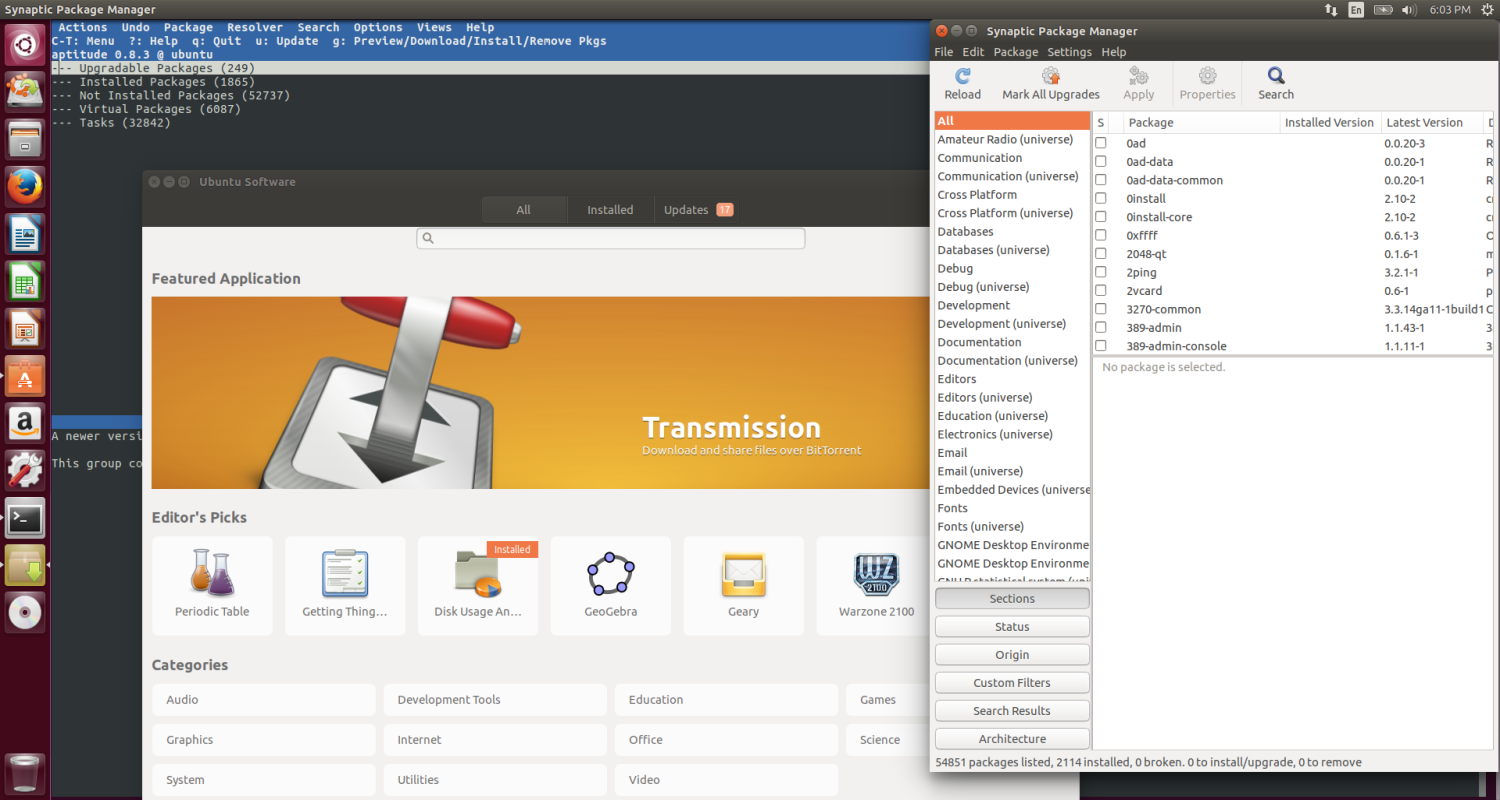
\includegraphics[width=\textwidth]{software_managers_ubuntu_deb.png}
\end{frame}

\begin{frame}{Graphical package managers II}{GNOME Software in Fedora and YaST in openSUSE}
  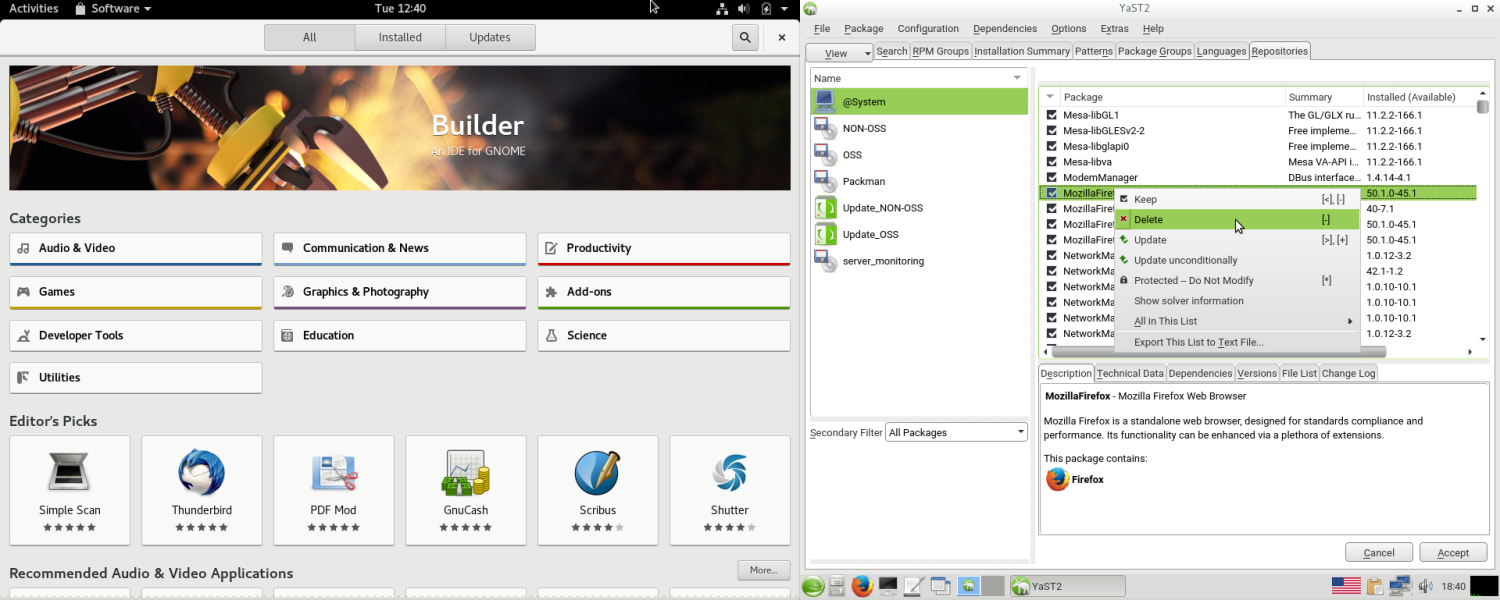
\includegraphics[width=\textwidth]{software_managers_fedora_suse.png}
  \begin{itemize}
    \item Practically every common general distribution has some graphical tool\ldots
  \end{itemize}
\end{frame}

\subsection{Compilation}

\begin{frame}[fragile]{Basics of compilation}
  \begin{itemize}
    \item Some software is distributed only as source code written in languages like C or C++ -- user has to compile it to get binary executable
    \item Compilation creates binary specific for particular operating system and hardware platform -- can be tuned for optimal performance
    \item Interpreted languages like Bash, Perl, Python or Java don't have to be compiled (but it is possible) -- they need their interpreter to run, relative easily portable among hardware platforms and OS
    \item Applications requiring compilation usually have good instructions
    \item If you don't have to do it, don't do it. Solving problems can be complicated -- contact someone skilled or author of the application\ldots
  \end{itemize}
  \begin{bashcode}
    # General schema within application directory with the source code:
    configure # Many possible parameters, settings for compilation
              # Not required in every time
    make # Basic building command, sometimes only this is required
    make install # Final creation of binary, sometimes required
  \end{bashcode}
\end{frame}

\begin{frame}[fragile]{Install tools needed for compilation}
  \begin{itemize}
    \item You need to install compilation tools for your distribution and programming languages you are going to use
    \item Commonly, extra dependencies are required to compile the application
    \begin{itemize}
      \item Packages for compilation use to end with \texttt{-dev} or \texttt{-devel} (e.g. if the software requires package \texttt{zlib} to run, install also its developmental version \texttt{zlib-dev(el)} to be able to compile it)
      \item All requirements should be listed in README or INSTALL documents of particular package -- user must install them manually\ldots
    \end{itemize}
  \end{itemize}
  \begin{bashcode}
    # openSUSE and SUSE Linux Enterprise
    zypper in -t pattern devel_basis devel_C_C++
    # Debian, Ubuntu and derivatives like Linux Mint and others
    apt-get install build-essential # Or "aptitude install build-essential"
    # Red Hat, CENTOS, Scientific Linux, Older Fedora and derivatives
    yum groupinstall "Development Tools" "C Development Tools and Libraries"
    # Fedora since version 22
    dnf group install "Development Tools" "C Development Tools and Libraries"
  \end{bashcode}
\end{frame}

\begin{frame}[fragile]{Compilation of RAxML}
  \begin{itemize}
    \item Available from \url{https://github.com/stamatak/standard-RAxML} (cite \href{https://bioinformatics.oxfordjournals.org/content/30/9/1312.abstract}{Stamakis 2014})
    \item Before compilation check \href{https://github.com/stamatak/standard-RAxML/blob/master/README}{README}
    \item This example does not require to run \texttt{make install}, it does not have extra dependencies for compilation, it requires specifying of particular source file by \texttt{make -f} (there are multiple \texttt{GCC} files, no one main)
  \end{itemize}
  \begin{bashcode}
    mkdir raxml # Create working directory
    cd raxml/ # Go there
    # Get source code from GitHub (svn downloads only changed files)
    svn co https://github.com/stamatak/standard-RAxML/tags/v8.2.9
    cd v8.2.9/ # Go to newly created directory
    ls # List files
    rm -rf Windows* # No need of Windows version - delete it
    # Compile standard version (other versions are available for better CPU)
    make -f Makefile.gcc
    rm *.o # Remove unneeded files (temporal for compilation)
    ./raxmlHPC -h # Launch it - see RAxML help
  \end{bashcode}
\end{frame}

\begin{frame}[fragile]{Compilation of SAMtools}
  \begin{itemize}
    \item See \url{http://www.htslib.org/download/}
    \item Ensure packages \texttt{zlib} and \texttt{zlib-dev(el)} are installed -- required for running and compilation, see \href{https://github.com/samtools/samtools/blob/1.3.1/INSTALL}{INSTALL} and \href{https://github.com/samtools/samtools/blob/1.3.1/README}{README}
  \end{itemize}
  \begin{bashcode}
    wget https://github.com/samtools/samtools/releases/download/1.3.1/
      samtools-1.3.1.tar.bz2 # Download SAMtools
    tar xjvf samtools-1.3.1.tar.bz2 # Unpack the archive
    cd samtools-1.3.1/ # Go to the unpacked directory
    ./configure # Configure settings for compilation
    ./configure --help # See various configuring options
    ./configure --without-curses # Compile without ncurses support
    make # Compile the software - check if there is error
         # Ensure developmental files for zlib (and ncurses) are available
    make install # Copy products into final location - default /usr/local
    make prefix=/where/to/install install # Install into custom location
    make prefix=/home/$USER/bin install # Binary is in /home/$USER/bin/bin
    make clean # Cleanup - final files are already in the destination
  \end{bashcode}
\end{frame}

\subsection{Java}

\begin{frame}[fragile]{Launching Java applications}
  \begin{itemize}
    \item \href{https://www.java.com/}{Java} is probably the most portable language working on any operating system -- the only condition is to install \href{https://en.wikipedia.org/wiki/Java_virtual_machine}{Java virtual machine (JVM)}
    \item Linux usually use \href{http://openjdk.java.net/}{OpenJDK} -- search for packages named \texttt{*openjdk*}
    \item Let's download e.g. \href{http://tree.bio.ed.ac.uk/software/figtree/}{FigTree} from \url{http://tree.bio.ed.ac.uk/download.php?id=90&num=3}
  \end{itemize}
  \begin{bashcode}
    # Go to directory where you downloaded it
    cd directory/with/downloaded/figtree
    # Decompress downloaded archive
    tar zxvf FigTree_v1.4.2.tgz
    # Go to created directory
    cd FigTree_v1.4.2/
    ls * # List files, also in subdirectories
    # Launch it (command java launches *.jar files)
    java -jar lib/figtree.jar
    # Limit its memory usage to 512 MB
    java -Xmx512m -jar lib/figtree.jar
  \end{bashcode}
\end{frame}

\subsection{Windows applications}

\begin{frame}[allowframebreaks]{Windows applications on Linux}
  \begin{itemize}
    \item Applications written for one operating system do not work on the other systems\ldots
    \begin{itemize}
      \item They must be written in portable language like Java or script like Perl, Python or BASH
      \item Otherwise we need an emulator -- not everything works
    \end{itemize}
    \item Windows 10 has \href{https://blogs.windows.com/buildingapps/2016/07/22/fun-with-the-windows-subsystem-for-linux/}{possibility to run Linux applications}, other option (for more Windows versions) is \href{https://www.cygwin.com/}{Cygwin} (application must be specially compiled to support Cygwin)
    \item To run Windows applications on Linux use \href{https://www.winehq.org/}{Wine}
    \begin{itemize}
      \item Search for packages named \texttt{wine} and install it
      \item Sometimes, extra functionality is in extra packages -- check \texttt{wine-*}
    \end{itemize}
    \item To run DOS application on Linux use \href{http://www.dosbox.com/}{dosbox} (package \texttt{dosbox})
    \item As soon as Wine is installed, just click to Windows \texttt{*.exe} file\ldots
    \item Windows applications are installed into \texttt{$\sim$/.wine/} where Windows directory structure is created, launchers use to be placed to standard application menu into \textbf{Wine} section
    \item Use \texttt{winecfg} to change settings (e.g. version of Windows -- can be different for each application, custom DLL library,~\ldots)
    \item \texttt{winefile} starts Windows file browser, \texttt{notepad} Notepad, \texttt{winemine} Mines
    \item To install some extra parts required by some applications use \texttt{winetricks}
    \begin{itemize}
      \item Usage use to differ according to distribution and GUI
      \item Browsing and selecting items to install can be bit messy\ldots
      \item It can be hard to check application requirements -- if it fails, check if it is listed at \url{https://appdb.winehq.org/} and/or run it from command line like \texttt{wine application.exe} and inspect errors in output
    \end{itemize}
    \item Before installing Windows application under Wine, check if there is some native Linux application to fit your needs\ldots
    \begin{itemize}
      \item Plenty of applications are available for more operating systems
      \item Linux distributions use to have external contributor's sites to provide more packages
      \item For many Windows-only applications there are fully comparable alternatives
    \end{itemize}
    \item Some applications do not work under Wine (from various reasons), some complex packages are \href{https://www.codeweavers.com/}{supported commercially} (I have no experience with it)
    \item Wine is well compatible with rest of the Linux hosting system, it is considerable to install Windows in e.g. WirtualBox (or another virtualization platform), if needed
  \end{itemize}
\end{frame}

\section{MetaCentrum}

\subsection{Information}

\begin{frame}[allowframebreaks]{CESNET and MetaCentrum}
  \begin{itemize}
    \item \href{https://www.cesnet.cz/?lang=en}{CESNET} is organization of Czech universities, Academy of Science and other organizations taking care about Czech backbone Internet, one of world leading institutions of this type
    \item CESNET provides various \href{https://www.cesnet.cz/services/?lang=en}{services}
    \begin{itemize}
      \item Massive computations -- \href{https://www.cesnet.cz/services/massive-computations-metacentrum/?lang=en}{MetaCentrum}
      \item Practically unlimited \href{https://www.cesnet.cz/services/data-storage/?lang=en}{data storage}
      \item \href{https://www.cesnet.cz/services/filesender/?lang=en}{FileSender} to be able to send up to 500~GB file
      \item \href{https://www.metacentrum.cz/en/Sluzby/MetaCloud/}{MetaCloud} -- computing (HPC) cloud similar to e.g. Amazon Elastic Compute Cloud (EC2) or Google Compute Engine
      \item \href{https://www.cesnet.cz/services/owncloud/?lang=en}{ownCloud} to backup and/or sync data across devices (default capacity is 100~GB, user may ask for more)
      \begin{itemize}
	\item It is possible to connect by webDAV to ownCloud (slide \ref{transfers}) -- many applications support it
	\item It is possible to share calendars and/or address books via claDAV and cardDAV among devices and/or people
      \end{itemize}
    \end{itemize}
    \item Services accessible without registration
    \begin{itemize}
      \item ownCloud \url{https://owncloud.cesnet.cz/}
      \item FileSender \url{https://filesender.cesnet.cz/}
      \item Go to web and log in with your institutional password
    \end{itemize}
    \item Services requiring registration (and approval)
    \begin{itemize}
      \item To use MetaCentrum fill registration form \url{https://metavo.metacentrum.cz/en/application/form}
      \item To use data storage fill registration form \url{https://einfra.cesnet.cz/perun-registrar-fed/?vo=storage&locale=en}
      \item After registration for MetaCentrum, user can join MetaCloud via \url{https://perun.metacentrum.cz/fed/registrar/?vo=meta&group=metacloud}
      \item Users not having access to \href{https://www.eduid.cz/en/index}{EduID} have to register first at HostelID \url{https://hostel.eduid.cz/en/index.html}
      \item Note some browser do not have required certificate and registration pages do not work correctly. \href{https://www.mozilla.org/firefox/}{Mozilla Firefox} should be safe choice every time.
    \end{itemize}
    \item Information about data storage \url{https://du.cesnet.cz/en/start} contains detailed usage instructions
    \item Information about MetaCentrum \url{https://www.metacentrum.cz/en/}
    \item Information about MetaCloud \url{https://wiki.metacentrum.cz/wiki/Kategorie:Clouds}
    \item Most of practical information for users are at wiki \url{https://wiki.metacentrum.cz/w/index.php?&setlang=en}
  \end{itemize}
\end{frame}

\begin{frame}{MetaCentrum}
  \begin{itemize}
    \item Also available is Galaxy \url{https://galaxy.metacentrum.cz/galaxy/} (same login as to MetaCentrum) -- web based bioinformatics framework (more information at \href{https://wiki.metacentrum.cz/wiki/Galaxy_application}{wiki})
    \item Current state and usage as available at \url{https://metavo.metacentrum.cz/en/}
    \item Manage your user account at \url{http://metavo.metacentrum.cz/en/myaccount/index.html}
    \item Personal view on actual resources and running tasks is at \url{https://metavo.metacentrum.cz/pbsmon2/person}
    \item List of available applications \url{https://wiki.metacentrum.cz/wiki/Kategorie:Applications}
    \item It has 8 front ends where users log and thousands of computers doing the calculations -- they are not accessed directly
    \item Most of computers are running \href{https://www.debian.org/}{Debian GNU/Linux}
  \end{itemize}
\end{frame}

\subsection{Usage}

\begin{frame}[fragile]{MetaCentrum usage}
  \begin{itemize}
    \item User can transfer data on one of \href{https://wiki.metacentrum.cz/wiki/Frontend}{frontends} by e.g. \texttt{scp} or \href{https://winscp.net/}{WinSCP} from Windows
    \item Same credentials are used for all front ends, for SSH login as well as file transmissions
  \end{itemize}
  \begin{bashcode}
    # Login to selected server (tarkil is located in Prague)
    ssh USER@tarkil.metacentrum.cz
    module add torque-client # Switch job scheduler to PBS Torque on tarkil
    # Continue as in any other command line...
    qsub ... # Submit the job (see later)
  \end{bashcode}
  \begin{itemize}
    \item In home directory on the server prepare all needed data and non-interactive script (interactive are more complicated) which will do the calculations
    \item Tasks are not launched immediately, but using \texttt{qsub} -- task is submitted into queue and system decides when it will be launched
  \end{itemize}
\end{frame}

\begin{frame}{File transfers to MetaCentrum}
  \begin{itemize}
    \item Graphical applications: \href{http://gftp.org/}{gFTP}, \href{https://filezilla-project.org/}{FileZilla} or from most of file managers
    \item Protocol is SSH/SSH2/SFTP/SCP, port 22, server is selected \href{https://wiki.metacentrum.cz/wiki/Frontend}{frontend's} address (e.g. \texttt{tarkil.metacentrum.cz}) -- it is recommendable to use all the time same frontend
    \item All servers are accessible under domain \texttt{*.metacentrum.cz}: \texttt{skirit}, \texttt{perian}, \texttt{onyx}, \texttt{zuphux} (located in Brno), \texttt{nympha}, \texttt{minos} (in Pilsen), and \texttt{tarkil} (in Prague) -- so that e.g. \texttt{tarkil.grid.cesnet.cz} is synonymous to \texttt{tarkil.metacentrum.cz}
    \item See slide \ref{transfers} and following to command-line transfers of files
  \end{itemize}
  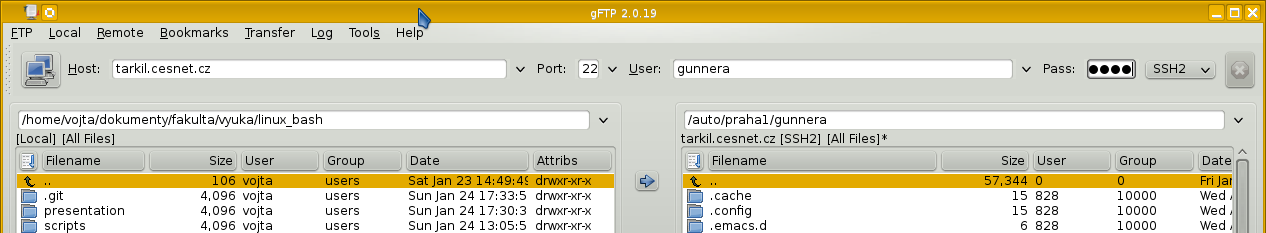
\includegraphics[width=\textwidth]{gftp.png}
\end{frame}

\subsection{Tasks}

\begin{frame}[fragile]{Basic skeleton of script running tasks I}
  \begin{bashcode}
    #!/bin/bash
    # Modify the script according to your needs!
    # Set data directories
    WORKDIR="bayes_batch" # Or something else
    DATADIR="/storage/praha1/home/$LOGNAME" # Or other storage
    # So there is directory /storage/praha1/home/gunnera/bayes_batch
    # (in this case) containing all the data needed for calculations
    # Clean-up of SCRATCH (it is temporal directory created by server) -
    # the commands will be launched on the end when the job is done
    trap 'clean_scratch' TERM EXIT
    trap 'cp -ar $SCRATCHDIR $DATADIR/ && clean_scratch' TERM
    # Prepare the task - copy all needed files from working directory
    # into particular computer which will finally do the calculations
    cp -ar $DATADIR/$WORKDIR/* $SCRATCHDIR/  || exit 1
    # Change working directory - script goes to the directory where
    # calculations are done
    cd $SCRATCHDIR/ || exit 2 # If it fails, exit script
  \end{bashcode}
  \vfill
  Ends on following slide\ldots
  \vfill
\end{frame}

\begin{frame}[fragile]{Basic skeleton of script running tasks II}
  \ldots begins on previous slide\ldots
  \vfill
  \begin{bashcode}
    # Prepare calculations - load required application modules
    # See https://wiki.metacentrum.cz/wiki/Kategorie:Applications
    # Every application module is loaded by "module add XXX"
    . /packages/run/modules-2.0/init/sh
    module add parallel # In this case GNU Parallel and MrBayes
    module add mrbayes-3.2.6
    # Launch the analysis - calculate MrBayes for multiple files
    # Note Parallel will distribute task among 8 CPU threads (-j 8),
    # so that qsub must in this case contain nodes=1:ppn=8 (see further)
    ls -1 *.nexus | parallel -j 8 'mb {} | tee -a {}.log'
    # Copy results back to home directory
    cp -ar $SCRATCHDIR $DATADIR/$WORKDIR || export CLEAN_SCRATCH=false
    # This is all needed, the script is ready to be launched...
    exit
  \end{bashcode}
  \begin{itemize}
    \item Make \texttt{metacentrum.sh} executable and modify it to fit your needs\ldots
    \item If it was written on Windows, convert EOL (and encoding)\ldots
  \end{itemize}
  \vfill
\end{frame}

\begin{frame}[fragile]{Launching of tasks}
  \begin{itemize}
    \item \url{https://wiki.metacentrum.cz/wiki/Running_jobs_in_scheduler}
    \item Personal view \url{https://metavo.metacentrum.cz/pbsmon2/person} has nice overview of available resources and tasks and allows comfortable construction of submission command
  \end{itemize}
  \begin{bashcode}
    # We will run up to 5 days, require 4 GB of RAM, 5 GB of disk space, one
    # physical computer with 8 CPU threads and we get all information mails
    qsub -l walltime=5d -l mem=4gb -l scratch=5gb -l nodes=1:ppn=8 -m abe \
      bayes_batch.sh
    # Check how the task is running (above web) and
    qstat | grep $USER
    qstat -u $USER
    qstat 123456789 # The task ID is available from commands above or mail
    qstat -f 123456789 # Print a lot of details
    qdel 123456789 # Terminate scheduled or running task
    qfree # List available resources
  \end{bashcode}
\end{frame}

\begin{frame}[allowframebreaks]{Scheduling details}
  \begin{itemize}
    \item \texttt{tarkil} is currently testing new scheduler \href{https://wiki.metacentrum.cz/wiki/PBS_Professional}{PBS Professional}
    \begin{itemize}
      \item It is using only limited number of machines, the syntax is slightly different from version described here
      \item Rather use for now another frontend or switch to old scheduler by \texttt{module add torque-client} and continue as usual (\texttt{qsub\ldots})
    \end{itemize}
    \item Specify needed time (up to 4 weeks; day, hours): \texttt{-l walltime=3w:4d:6h}, \texttt{-l walltime=6d:18h},~\ldots
    \begin{itemize}
      \item User \href{mailto:meta@cesnet.cz}{can ask} to prolonge the walltime
    \end{itemize}
    \item Ask for as much RAM as you need (e.g. \texttt{-l mem=8gb})
    \begin{itemize}
      \item If the task is going to require more, than allowed, system kills it\ldots
      \item If user doesn't use all required RAM, the system temporarily lowers priority for future tasks
      \item It can be hard to estimate\ldots
    \end{itemize}
    \item Disk space is relatively free resource, user can ask more to have some reserve (e.g. \texttt{-l scratch=10gb})
    \item Specify how many physical computer you are going to use (e.g. \texttt{-l nodes=1} for one machine) and number of CPU threads on each machine (e.g. \texttt{-l nodes=1:ppn=8} for 1~machine with 8~cores or \texttt{-l nodes=2:ppn=4} for 2~machines, each with 4~CPU threads)
    \begin{itemize}
      \item It use to be necessary to specify correct number of threads for the application (e.g. \texttt{parallel -j 4}) -- the application sees all CPUs on the machine, but can't use them
      \item If the application consumes less than required, the system temporarily lowers priority for future tasks, if it try to use more, it will be very slowed down
      \item If using more physical machines, ensure correct settings of e.g. MPI
    \end{itemize}
    \item If requesting e-mails (e.g. \texttt{-m abe} to get mail about submission, starting and termination of the task) and submitting plenty of tasks by some script, it can result in hundreds of mails -- mail servers don't like it\ldots
    \item Every user has certain \href{https://metavo.metacentrum.cz/pbsmon2/users/}{priority} highered by acknowledgments in publications to MetaCentrum and lowered by intensive usage of the service (the usage is calculated from past month)
    \item After submission of the task, check in \href{https://metavo.metacentrum.cz/pbsmon2/queues/jobsQueued}{the queue} in which state it is -- sometimes it can't start because of impossible combination of resources or so
    \item User can \href{https://metavo.metacentrum.cz/pbsmon2/nodes/physical}{check load of machines}
  \end{itemize}
\end{frame}

\begin{frame}{Common problems with launching the tasks}
  \begin{itemize}
    \item Script fails because of wrong PATH or missing file -- ensure all needed files are transferred and applications receive correct paths
    \begin{itemize}
      \item Do not use absolute paths (starting with \texttt{/}) -- only relative
    \end{itemize}
    \item Not all required applications are correctly loaded
    \begin{itemize}
      \item Check \href{https://wiki.metacentrum.cz/wiki/Kategorie:Applications}{wiki} and load all needed applications
      \item Names of binaries are commonly little bit different -- contain names of versions etc
    \end{itemize}
    \item Estimation of time needed to run the task
    \begin{itemize}
      \item No really good solution\ldots
      \item Make some trials and try to estimate\ldots
      \item There are very different CPUs available (with different speeds) -- it is possible to require particular CPU type (but it reduces number of available nodes\ldots)
    \end{itemize}
  \end{itemize}
\end{frame}

\begin{frame}[fragile]{Get to task's working directory}
  \begin{itemize}
    \item Go to \url{https://metavo.metacentrum.cz/pbsmon2/person} and click to list of your tasks and click to selected task
    \item Search for information \textbf{exec\_host} (address of node doing the task) and \textbf{SCRATCHDIR} (temporal directory for all data and results)
    \item Sometimes one needs to monitor task progress or influence it
    \item It is not possible to directly modify running task, but at least check (and possibly modify) input data and see outputs
  \end{itemize}
  \begin{bashcode}
    # From MetaCentrum frontend login to respective node running the task
    ssh exec_host # No need to specify user name
    # Go to SCRATCH directory
    cd SCRATCHDIR
    # There are working data of currently running task...
  \end{bashcode}
\end{frame}

\begin{frame}[fragile]{Interactive tasks}
  \begin{itemize}
    \item See information at \url{https://wiki.metacentrum.cz/wiki/Interactive_job}
  \end{itemize}
  \begin{bashcode}
    # Again launch qsub according to actual needs
    # Note "-I" for interactive session and missing script name
    qsub -I -l walltime=2h -l nodes=1:ppn=1 -l mem=2gb
    # Wait for job to start..
    # After we get the interactive task, we are on new server
    hostname # See where we are - we can connect to that server directly
    ssh USER@given.server.cz # User name and password are the same
                             # Server address is output from "hostname"
    screen # Secure we can log off in the meantime
  \end{bashcode}
  \begin{itemize}
    \item Work as on normal Linux server\ldots
    \item With \texttt{screen} we can disconnect as usually and let tasks run in background
  \end{itemize}
\end{frame}

\subsection{Graphical connection}

\begin{frame}[fragile]{Graphical interactive task}
  \begin{itemize}
    \item See information at \url{https://wiki.metacentrum.cz/wiki/Remote_desktop}
  \end{itemize}
  \begin{bashcode}
    # Again launch qsub according to actual needs
    # Note "-I" for interactive session and missing script name
    qsub -I -l walltime=2h -l nodes=1:ppn=1 -l mem=2gb
    # Wait for job to start..
    # After we get the interactive task, we are on new server
    screen # Secure we can log off in the meantime
    module add gui # We need to add GUI module
    gui start # Start GUI (see above link for details)
    gui info -p # Print information about running VNC sessions
                # Including address, port and password to connect
  \end{bashcode}
  \begin{itemize}
    \item Launch your favorite VNC client (\href{https://www.kde.org/applications/internet/krdc/}{KRDC}, \href{http://www.tightvnc.com/}{TightVNC},~\ldots) and use credentials from above output to connect
    \item Work as on normal Linux desktop\ldots
    \item With \texttt{screen} we can disconnect as usually
  \end{itemize}
\end{frame}

\begin{frame}{Running VNC}
  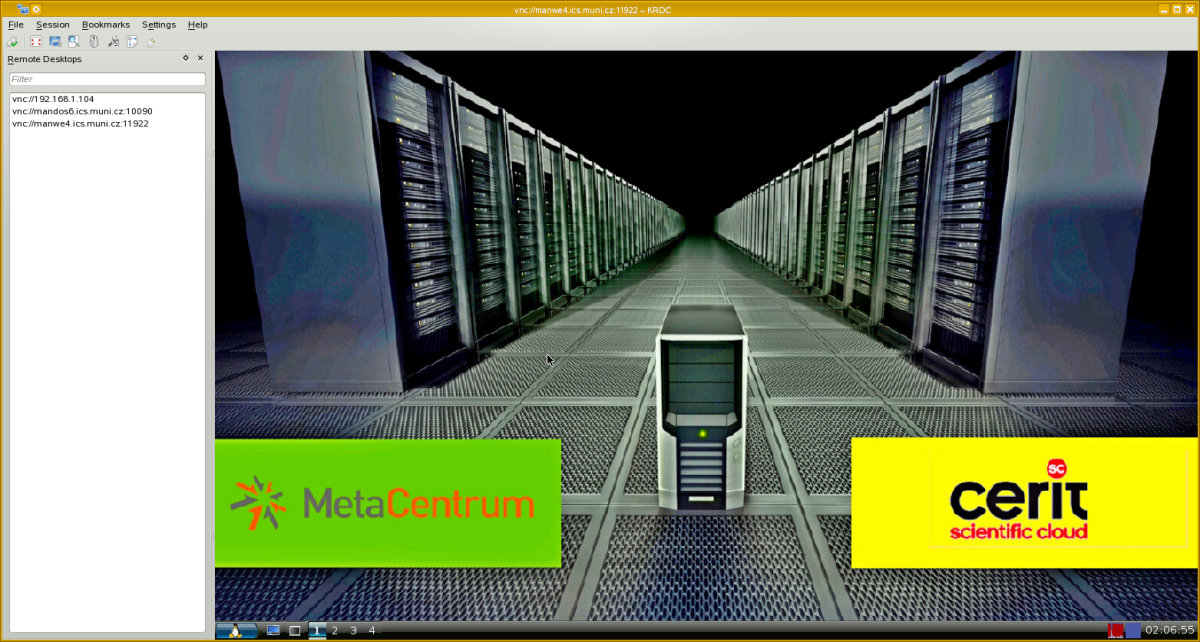
\includegraphics[width=\textwidth]{vnc.png}
\end{frame}

\section{Administration}

% \begin{frame}{Btrfs and Snapper} % TODO Btrfs, Snapper
%   \begin{itemize}
%     \item 
%   \end{itemize}
% \end{frame}

\subsection{System services}

\begin{frame}[fragile]{Managing system services}
  \begin{itemize}
    \item Different among distributions -- several main methods
    \item In Linux, most common is \href{https://wiki.freedesktop.org/www/Software/systemd/}{SystemD}, less common older init scripts and RC scripts
    \item Mac OS~X and various BSD and other systems have different methods
    \item Used to manage system services like networking, cron, web server, database,~\ldots
    \item \alert{Read documentation for your distribution!}
    \item Most of actions require root authentication
  \end{itemize}
  \begin{bashcode}
    # SystemD - huge amount of possibilities
    systemctl enable/disable/status/start/stop servicename # TAB helps
    # RC scripts
    rcservicename status/start/stop # TAB helps to select service
    # Init scripts
    /etc/init.d/servicename status/start/stop # TAB helps to select service
  \end{bashcode}
\end{frame}

\begin{frame}[fragile]{SystemD usage}
  \begin{bashcode}
    # List installed services and their status
    systemctl list-units --type service
    # Enable/disable/see status/start/stop/restart/... service
    systemctl enable/disable/status/start/stop/restart servicename # TAB...
    # Show overriden config files
    systemd-delta
    # Analyze boot time (how long does each service take to start)
    systemd-analyze blame # Text output
    systemd-analyze plot > filename.svg # Same in graphics
    # Log for particular service
    journalctl -u servicename
    # Last logged messages (press Ctrl+C to exit)
    journalctl -f
    # Log records since last boot
    journalctl -b
    # Time and date information and management
    timedatectl
  \end{bashcode}
\end{frame}

\section{Git}

\begin{frame}[fragile]{Git and GitHub}
  \begin{itemize}
    \item \href{https://git-scm.com/}{Git} is \href{https://en.wikipedia.org/wiki/Version_control}{version controlling} system -- it traces changes among all versions -- absolutely crucial for any software development
    \item \href{https://github.com/}{GitHub} is currently probably the most popular platform to host development of open-source projects, see \href{https://help.github.com/}{documentation}
    \item Older (nowadays not so common) version controlling systems is Subversion (SVN), there are many more
    \item Probably the best textbook for Git is \href{https://git-scm.com/book/en/v2}{Chacon's Pro Git}
    \begin{itemize}
      \item Dostupná i~\href{https://git-scm.com/book/cs/v2}{česky} (včetně \href{https://knihy.nic.cz/}{prvního vydání})
    \end{itemize}
    \item Changes and their history is stored in repository (local or network, shared or private) -- it is possible to view any historical state and differences between any versions
    \item It is possible to trace who and when did what
    \item Branching and merging of branches helps with making of big changes
  \end{itemize}
\end{frame}

\begin{frame}[fragile]{Git principles}
  \begin{multicols}{2}
    \begin{itemize}
      \item Three main areas
      \begin{enumerate}
	\item Working directory
	\item Staging (changes awaiting to be pushed to the repository)
	\item Git repository (remote/local)
      \end{enumerate}
      \item Everyone has whole repository and history -- very robust
      \item Flexible branches
      \begin{itemize}
	\item Very convenient
	\item Keeping work structured
	\item Separation of tasks
	\item Keeping more versions of the project in parallel
      \end{itemize}
    \end{itemize}
    \begin{center}
      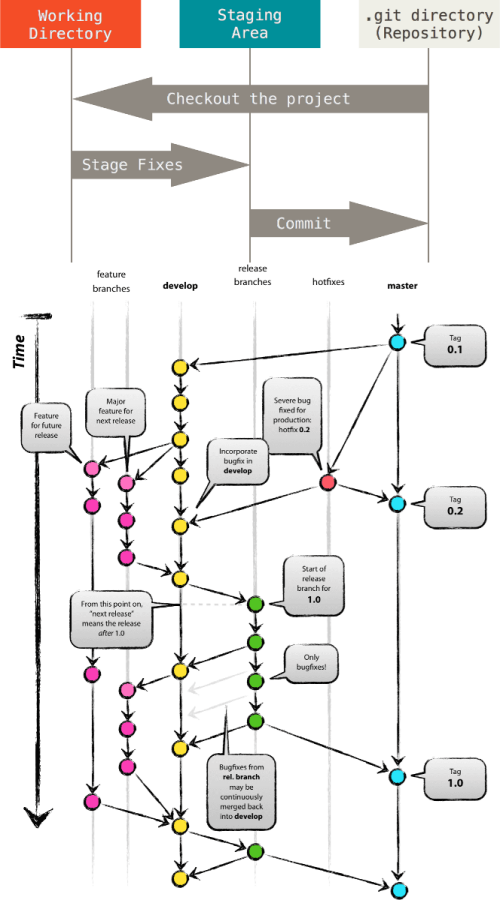
\includegraphics[height=5.75cm]{git.png}
    \end{center}
    \begin{flushright}
      \begin{footnotesize}
	\href{https://git-scm.com/book/en/v2/Getting-Started-Git-Basics}{https://git-scm.com/}, \href{http://nvie.com/posts/a-successful-git-branching-model/}{http://nvie.com/}
      \end{footnotesize}
    \end{flushright}
  \end{multicols}
\end{frame}

\begin{frame}[fragile]{Working with Git -- start and sending changes}
  \begin{bashcode}
    # Create a new repository for new project
    git init # No need when cloning from existing repository
    # Or checkout (make a copy) for another local or remote repository
    git clone /path/to/local/repository # Locally mounted repository
    git clone username@host:/path/to/remote/repository # Over SSH
    git clone https://github.com/V-Z/course-linux-command-line-bash-
      scripting-metacentrum.git # Clone from web, e.g. GitHub
    # Add files to trace with Git
    # Ignored files (or patterns) can be listed in .gitignore file
    git add <files> # Or "git add *"
    # Commit changes to prepare then to send to repository
    git commit -m "Message..."
    # If you did not start by cloning, add connection to server
    git remote add origin <location> # Do only once on the beginning
    # <location> can be remote server or local path
    git remote add origin . # For repository within working directory
    # Push changes into the (regardless where it is) repository
    git push origin master # See further for selection of branches
  \end{bashcode}
\end{frame}

\begin{frame}[fragile]{Working with Git -- branching and getting changes}
  \begin{bashcode}
    # Making new branch and switching to it
    git checkout -b NewFeature # Now we are in branch NewFeature
    # Switch back to branch master
    git checkout master # Generally, "git checkout <branch>"
    # Delete the branch (changes there are lost, must be in another branch)
    git branch -d NewFeature # Delete local branch, to delete remote do:
    git push origin --delete <branch>
    # Branch must be also pushed to the remote server
    git push origin <branch>
    # List branches (current is marked by asterisk on the beginning)
    git branch
    # Update local repository to the newest version from central repository
    git pull # Fetch and merge remote changes
    # Merge another branch into the current one
    git merge <branch>
    # In case of conflict, git shows editor and user must fix it manually
    git add <file with conflict> # Needed to re-add conflicting file
    # To see changes before merging
    git diff <source_branch> <target_branch>
  \end{bashcode}
\end{frame}

\begin{frame}[fragile]{Working with Git -- tags, logs and settings}
  \begin{bashcode}
    # Tagging e.g. milestones, released versions of software, etc.
    git tag <name> <commit id> # <name> can be custom, <commit id> from log:
    git log # Newest is on top, see also "git log --help"
    git log --graph --oneline --decorate --all # Full long log
    # Discard local changes for particular file
    git checkout -- <file>
    # Discard all local changes
    git fetch origin # Overwrite local changes
    git reset --hard origin/master # If local repository is broken...
    gitk # Graphical interface
    git config color.ui true # Set output to be colored
    git config format.pretty oneline # Nicer log output
    ~/.git # Contains user's settings, .git in every repository contains
           # data and settings for particular repository
  \end{bashcode}
\end{frame}

\section{The End}

% \subsection{Switching to Linux} % TODO Switching

% \begin{frame}{Brief list of applications to help to switch to Linux}
%   \begin{itemize}
%     \item 
%   \end{itemize}
% \end{frame}

\subsection{Resources}

\begin{frame}[allowframebreaks]{Resources to learn to work in the terminal}
  \begin{itemize}
    \item openSUSE (general handbook) \url{https://doc.opensuse.org/documentation/leap/startup/html/book.opensuse.startup/part.bash.html}
    \item Ubuntu (general handbook) \url{https://help.ubuntu.com/community/UsingTheTerminal}
    \item BASH full reference manual \url{https://www.gnu.org/software/bash/manual/} (advanced)
    \item Debian (general handbook) \url{https://www.debian.org/doc/manuals/debian-reference/ch01.en.html}
    \item Guide to Unix \url{https://en.wikibooks.org/wiki/Guide_to_Unix}
    \item BASH for beginners \url{http://tldp.org/LDP/Bash-Beginners-Guide/html/Bash-Beginners-Guide.html} (the site has plenty of good resources)
    \item BASH Guide for Beginners \url{http://linuxcourse.rutgers.edu/documents/Bash-Beginners-Guide/}
    \item Linux tutorial \url{http://ryanstutorials.net/linuxtutorial/}
    \item Getting Started with BASH \url{http://www.hypexr.org/bash_tutorial.php}
    \item Bash Guide \url{http://mywiki.wooledge.org/BashGuide}
    \item Učebnice Linuxu \url{https://www.abclinuxu.cz/ucebnice}
  \end{itemize}
\end{frame}

\begin{frame}{Manuals for package management}
  \begin{itemize}
    \item openSUSE AND SUSE Linux Enterprise: \url{https://doc.opensuse.org/documentation/leap/startup/html/book.opensuse.startup/part.reference.software.html} and \url{https://en.opensuse.org/Zypper}
    \item Red Hat, Fedora, CENTOS, Scientific Linux and others: \url{http://yum.baseurl.org/}
    \item Debian (and derivatives): \url{https://www.debian.org/doc/manuals/debian-reference/ch02.en.html} and \url{https://wiki.debian.org/PackageManagement}
    \item Ubuntu (and derivatives): \url{https://help.ubuntu.com/stable/ubuntu-help/addremove.html} and \url{https://help.ubuntu.com/community/AptGet/Howto}
    \item And another distributions\ldots
  \end{itemize}
\end{frame}

\begin{frame}[allowframebreaks]{How to ask for help}
  \label{howtoask}
  \begin{itemize}
    \item \alert{Never ever} ask simple silly lazy questions you can quickly find in manual or web
    \item People on mailing lists and forums respond volunteerly in their spare free time -- do not waste it -- be polite, brief and informative
    \item Be as specific and exact as possible
    \begin{itemize}
      \item Write \alert{exactly} what you did (``It doesn't work!'' is useless\ldots)
      \item Copy/paste your commands and their output, especially error messages -- they are keys to solve the problem
      \item Try to search web for the error messages (or their parts)
      \item Try to provide minimal working example -- add at least part of your data (if applicable) so that the problem is reproducible
      \item Specify name version(s) of distribution ans problematic software
    \end{itemize}
    \item \textbf{OSS is free as freedom of speech -- not as free beer!}
    \begin{itemize}
      \item As soon as you don't pay for support, you can't blame anyone for lack of responses
      \item There are plenty of reasons some software doesn't work -- usage/data author didn't expect, unsupported version of operating system, author's mistake, user's mistake,~\ldots
      \item Authors wish their software to be useful -- constructive feedback, reporting bugs and wishes is welcomed, but it must be provided in the way useful for the developer
    \end{itemize}
    \item Imagine you should answer -- which information do you need?
    \item Try to find the best place to ask your question -- specific forum for particular distribution or software use to be the best option
    \item Learning command line is like learning foreign language\ldots
  \end{itemize}
\end{frame}

\begin{frame}{Main general fora}
  \begin{itemize}
    \item Probably the best are fora from StackExchange \url{https://stackexchange.com/sites}
    \item General forum for programmers \url{https://stackoverflow.com/}
    \item UNIX forum \url{https://unix.stackexchange.com/}
    \item Forum for administrators \url{https://superuser.com/}
  \end{itemize}
\end{frame}

\begin{frame}{openSUSE}
  \begin{itemize}
    \item Homepage \url{https://www.opensuse.org/}
    \item Wiki \url{https://en.opensuse.org/Main_Page}, documentation \url{https://doc.opensuse.org/}
    \item News \url{https://news.opensuse.org/}, developers' blogs \url{https://lizards.opensuse.org/}, blogs \url{http://planet.opensuse.org/}
    \item Forums \url{https://forums.opensuse.org/}, mailing lists \url{https://lists.opensuse.org/}
    \item Community \url{http://opensuse-community.org/}, guide \url{http://opensuse-guide.org/}
  \end{itemize}
\end{frame}

\begin{frame}{Debian, Ubuntu, Linux Mint and derivatives}
  \begin{itemize}
    \item Debian \url{https://www.debian.org/}
    \item Ubuntu \url{https://www.ubuntu.com/}, support \url{https://www.ubuntu.com/support}, Ask ubuntu \url{https://askubuntu.com/}
    \item Kubuntu \url{http://www.kubuntu.org/}, forum \url{https://www.kubuntuforums.net/}
    \item Xubuntu \url{http://xubuntu.org/}, Lubuntu \url{http://lubuntu.net/}
    \item Linux Mint \url{https://www.linuxmint.com/}
  \end{itemize}
\end{frame}

\begin{frame}{Fedora}
  \begin{itemize}
    \item Homepage \url{https://getfedora.org/}
    \item Official forum \url{https://ask.fedoraproject.org/}
    \item Documentation \url{https://docs.fedoraproject.org/}
    \item Community forum \url{http://fedoraforum.org/}
  \end{itemize}
\end{frame}

\begin{frame}{KDE and LibreOffice}
  \begin{itemize}
    \item LibreOffice \url{https://www.libreoffice.org/}, Document Foundation \url{https://www.documentfoundation.org/}
    \item KDE \url{https://www.kde.org/}, forum \url{https://forum.kde.org/}, application store \url{https://store.kde.org/}, KDE for education \url{https://edu.kde.org/}, blogs \url{https://planetkde.org/}
  \end{itemize}
\end{frame}

\begin{frame}{České weby -- zdroje informací a fóra}
  \begin{itemize}
    \item ABC Linuxu \url{https://www.abclinuxu.cz/}
    \item Root \url{https://www.root.cz/}
    \item LinuxExpres \url{https://www.linuxexpres.cz/}
    \item LinuxDays (největší konference) \url{https://www.linuxdays.cz/}
    \item OpenOffice/LibreOffice \url{https://www.openoffice.cz/} a~\url{https://www.knihaoffice.cz/}
    \item Ubuntu \url{http://www.ubuntu.cz/}, wiki \url{http://wiki.ubuntu.cz/}, fórum \url{http://forum.ubuntu.cz/}, Kubuntu \url{http://www.kubuntu.cz/}, Lubuntu \url{http://www.lubuntu.cz/}, Xubuntu \url{http://www.xubuntu.cz/}
    \item Fedora \url{https://mojefedora.cz/}, příručka \url{https://wiki.mojefedora.cz/doku.php?id=navody:prirucka:obsah}
    \item openSUSE \url{http://www.opensuse.cz/}
    \item Linux Mint \url{https://www.linux-mint-czech.cz/}
  \end{itemize}
\end{frame}

\subsection{The very end}

\begin{frame}{The end}{Our course is over\ldots}
  \begin{center}
    \ldots I hope it was helpful for You\ldots
    \vfill
    \ldots any feedback is welcomed\ldots
    \vfill
    \ldots happy Linux hacking\ldots
    \vfill
    \ldots any final questions?
    \vfill
  \end{center}
  \begin{flushright}
    \begin{tiny}
    \href{https://en.wikipedia.org/wiki/XeTeX}{Typesetting} using \XeLaTeX~on \href{https://www.opensuse.org/}{openSUSE} \href{https://en.wikipedia.org/wiki/GNU}{GNU}/\href{https://en.wikipedia.org/wiki/Linux}{Linux} \today
    \end{tiny}
  \end{flushright}
\end{frame}

\end{document}

% TODO Missing topics
% * Security, antiviruses
% * GUI
% * More examples about software on MetaCentrum, scripts (on MetaCentrum)
% * More about regular expressions
% * AWK: https://www.gnu.org/software/gawk/manual/ http://www.grymoire.com/Unix/Awk.html https://en.wikibooks.org/wiki/An_Awk_Primer
